% !TeX encoding = UTF-8
% !TeX program = xelatex
% !TeX spellcheck = en_US

\documentclass[degree=master,degree-type=professional]{thuthesis}
  % 学位 degree:
  %   doctor | master | bachelor | postdoc
  % 学位类型 degree-type:
  %   academic(默认)| professional
  % 语言 language
  %   chinese(默认)| english
  % 字体库 fontset
  %   windows | mac | fandol | ubuntu
  % 建议终版使用 Windows 平台的字体编译


% 论文基本配置,加载宏包等全局配置
% !TeX root = ./thuthesis-example.tex

% 论文基本信息配置

\thusetup{
  %******************************
  % 注意:
  %   1. 配置里面不要出现空行
  %   2. 不需要的配置信息可以删除
  %   3. 建议先阅读文档中所有关于选项的说明
  %******************************
  %
  % 输出格式
  %   选择打印版(print)或用于提交的电子版(electronic),前者会插入空白页以便直接双面打印
  %
  output = print,
  %
  % 标题
  %   可使用“\\”命令手动控制换行
  %
  title  = {基于深度学习的骨髓血细胞检测与识别技术研究},
  title* = {Research on bone marrow blood cell detection and recognition based on deep learning},
  %
  % 学位
  %   1. 学术型
  %      - 中文
  %        需注明所属的学科门类,例如:
  %        哲学、经济学、法学、教育学、文学、历史学、理学、工学、农学、医学、
  %        军事学、管理学、艺术学
  %      - 英文
  %        博士:Doctor of Philosophy
  %        硕士:
  %          哲学、文学、历史学、法学、教育学、艺术学门类,公共管理学科
  %          填写“Master of Arts“,其它填写“Master of Science”
  %   2. 专业型
  %      直接填写专业学位的名称,例如:
  %      教育博士、工程硕士等
  %      Doctor of Education, Master of Engineering
  %   3. 本科生不需要填写
  %
  degree-name  = {工学硕士},
  degree-name* = {Master of Science},
  %
  % 培养单位
  %   填写所属院系的全名
  %
  department = {电子工程系},
  %
  % 学科
  %   1. 学术型学位
  %      获得一级学科授权的学科填写一级学科名称,其他填写二级学科名称
  %   2. 工程硕士
  %      工程领域名称
  %   3. 其他专业型学位
  %      不填写此项
  %   4. 本科生填写专业名称,第二学位论文需标注“(第二学位)”
  %
  discipline  = {电子与通信工程},
  discipline* = {Electronics and Communication Engineering},
  %
  % 姓名
  %
  author  = {孙天宇},
  author* = {Sun Tianyu},
  %
  % 指导教师
  %   中文姓名和职称之间以英文逗号“,”分开,下同
  %
  supervisor  = {杨健, 教授},
  supervisor* = {Professor Yang Jian},
  %
  % 副指导教师
  %
  % associate-supervisor  = {陈文光, 教授},
  % associate-supervisor* = {Professor Chen Wenguang},
  %
  % 联合指导教师
  %
  % co-supervisor  = {某某某, 教授},
  % co-supervisor* = {Professor Mou Moumou},
  %
  % 日期
  %   使用 ISO 格式;默认为当前时间
  %
  % date = {2019-07-07},
  %
  % 是否在中文封面后的空白页生成书脊(默认 false)
  %
  include-spine = false,
  %
  % 密级和年限
  %   秘密, 机密, 绝密
  %
  % secret-level = {秘密},
  % secret-year  = {10},
  %
  % 博士后专有部分
  %
  % clc                = {分类号},
  % udc                = {UDC},
  % id                 = {编号},
  % discipline-level-1 = {计算机科学与技术},  % 流动站(一级学科)名称
  % discipline-level-2 = {系统结构},          % 专业(二级学科)名称
  % start-date         = {2011-07-01},        % 研究工作起始时间
}

% 载入所需的宏包

% 定理类环境宏包
\usepackage{amsthm}
% 也可以使用 ntheorem
% \usepackage[amsmath,thmmarks,hyperref]{ntheorem}

\thusetup{
  %
  % 数学字体
  % math-style = GB,  % GB | ISO | TeX
  math-font  = xits,  % stix | xits | libertinus
}

% 可以使用 nomencl 生成符号和缩略语说明
% \usepackage{nomencl}
% \makenomenclature

% 表格加脚注
\usepackage{threeparttable}
\usepackage{makecell}
% 表格中支持跨行
\usepackage{multirow}

% 固定宽度的表格。
% \usepackage{tabularx}

% 跨页表格
\usepackage{longtable}


% 算法
\usepackage{algorithm}
\usepackage{algorithmic}

% 量和单位
\usepackage{siunitx}
\usepackage{float} 
\usepackage{subcaption}

% 参考文献使用 BibTeX + natbib 宏包
% 顺序编码制
\usepackage[sort]{natbib}
\bibliographystyle{thuthesis-numeric}

% 著者-出版年制
% \usepackage{natbib}
% \bibliographystyle{thuthesis-author-year}

% 本科生参考文献的著录格式
% \usepackage[sort]{natbib}
% \bibliographystyle{thuthesis-bachelor}

% 参考文献使用 BibLaTeX 宏包
% \usepackage[style=thuthesis-numeric]{biblatex}
% \usepackage[style=thuthesis-author-year]{biblatex}
% \usepackage[style=apa]{biblatex}
% \usepackage[style=mla-new]{biblatex}
% 声明 BibLaTeX 的数据库
% \addbibresource{ref/refs.bib}

% 定义所有的图片文件在 figures 子目录下
\graphicspath{{figures/}}

% 数学命令
\makeatletter
\newcommand\dif{%  % 微分符号
  \mathop{}\!%
  \ifthu@math@style@TeX
    d%
  \else
    \mathrm{d}%
  \fi
}
\makeatother

% hyperref 宏包在最后调用
\usepackage{hyperref}



\begin{document}

% 封面
\maketitle

% 学位论文指导小组、公开评阅人和答辩委员会名单
% 本科生不需要
% !TeX root = ../thuthesis-example.tex

\begin{committee}[name={学位论文指导小组、公开评阅人和答辩委员会名单}]

  \newcolumntype{C}[1]{@{}>{\centering\arraybackslash}p{#1}}

  \section*{指导小组名单}

  \begin{center}
    \begin{tabular}{C{3cm}C{3cm}C{9cm}@{}}
      杨健 & 教授     & 清华大学 \\
    \end{tabular}
  \end{center}


  \section*{公开评阅人名单}

  \begin{center}
    \begin{tabular}{C{3cm}C{3cm}C{9cm}@{}}
      刘XX & 教授   & 清华大学                    \\
      杨XX & 研究员 & 中国XXXX科学院XXXXXXX研究所 \\
    \end{tabular}
  \end{center}


  \section*{答辩委员会名单}

  \begin{center}
    \begin{tabular}{C{2.75cm}C{2.98cm}C{4.63cm}C{4.63cm}@{}}
      主席 & 赵XX                  & 教授                    & 清华大学       \\
      委员 & 刘XX                  & 教授                    & 清华大学       \\
          & \multirow{2}{*}{杨XX} & \multirow{2}{*}{研究员} & 中国XXXX科学院 \\
          &                       &                         & XXXXXXX研究所  \\
          & 黄XX                  & 教授                    & XXXX大学       \\
          & 周XX                  & 副教授                  & XXXX大学       \\
      秘书 & 吴XX                  & 博士              & 清华大学       \\
    \end{tabular}
  \end{center}

\end{committee}



% 也可以导入 Word 版转的 PDF 文件
% \begin{committee}[file=figures/committee.pdf]
% \end{committee}


% 使用授权的说明
\copyrightpage
% 将签字扫描后授权文件 scan-copyright.pdf 替换原始页面
% \copyrightpage[file=scan-copyright.pdf]

\frontmatter
% !TeX root = ../thuthesis-example.tex

% 中英文摘要和关键字

\begin{abstract}
白血病是一种常见多发且较为凶险的血液疾病,其早期发现与治疗至关重要。
目前白血病的临床诊断主要依靠医师对骨髓穿刺涂片进行形态学检查。
人工镜检存在着繁琐费时、结果主观性强等缺点,并且培养病理诊断医师要耗费大量时间。
近年来,计算机科学技术高速发展,人工智能技术被广泛应用于医学领域,其高效的计算与分析能力为疾病诊疗
带来了深刻的变革。目前诸多研究学者开始研究基于深度学习的方法来自动定位与识别血细胞,上述研究主要是通过目标检测识别网络进行迁移学习,
缺少对于骨髓血细胞特性的定制化改进。因此,我们与邃蓝智能科技 (上海) 有限公司进行合作,
针对骨髓血细胞检测与识别关键问题进行研究,提高骨髓血细胞检测识别算法精度,并编写相关软件,为医生的临床诊断提供参考依据。

首先,在数据方面,我们采用主动学习技术实现了骨髓血细胞数据标注迭代框架,并在医生的协作下快速完成了多批次骨髓血细胞
边界框与类别信息的标注。在骨髓血细胞检测方面,我们对比了多种单阶段与双阶段目标检测网络,将性能优异RetinaNet作为基线模型。
我们对比了RetinaNet网络在仅检测与检测识别一体化任务上准确率的差异,并确定了先检测再识别的骨髓血细胞处理流程。
针对密集、堆叠与黏连骨髓血细胞区域的漏检、错检等问题,我们提出了全局注意力自下而上路径聚合网络结构,IOU预测分支与
最优输运的全局最优标签分配策略,改进方法平均检测精度相比于主流目标检测网络提升了1\% 以上,达到了较为先进的性能。
在骨髓血细胞识别方面,我们基于Vision Transformer网络实现了骨髓血细胞的细粒度识别。
在该方法中,我们采用基于滑动窗的图像块划分方法,保留局部细节信息。此外,我们提出了辨识性区域选择模块,引导网络对细胞核、
细胞质等细微差异区域进行聚焦。引入了对比损失,约束骨髓血细胞的类间差异性与类内聚集性。
该方法在慕尼黑骨髓血细胞数据集上的平均分类准确率为 91.96\%,相比于基线模型提升了0.74\%。
最后,我们基于B/S架构设计并开发了骨髓血细胞检测与识别软件,将上述骨髓血细胞检测识别算法进行落地部署,
软件可以自动完成骨髓血细胞的定位与分类计数,用于辅助医生临床诊断。




  % 关键词用“英文逗号”分隔,输出时会自动处理为正确的分隔符
  \thusetup{
    keywords = {医学图像分析, 骨髓血细胞, 深度学习, 检测识别},
  }
\end{abstract}

\begin{abstract*}
Leukemia is a common, multiple and dangerous blood disease, whose early diagnosis and treatment are
crucial to prolong the survival time and improve the quality of patients' live. 
At present, the clinical diagnosis of leukemia mainly relies on the morphological examination of bone marrow aspiration smear by physicians.
Manual microscopic examination is very cumbersome and time-consuming and the results are highly subjective. In addition, it takes a lot of time to train experienced pathologists.
The computer science and technology has ballooned in recent years. Artificial intelligence technology has been widely used in the medical field. Its efficient computing and analysis capabilities 
have brought profound changes to the diagnosis and treatment of diseases. 
At present, many researchers have begun to study methods based on deep learning to automatically locate and identify blood cells. 
The above researches are mainly based on general-purpose target detection and recognition networks 
and lack improvements for the characteristics of bone marrow blood cells.
Therefore, we cooperate with Deep Voxel Intelligent Technology to research the key issues of bone marrow blood cell 
detection and recognition. We aims to improve the accuracy of bone marrow blood cell detection and recognition and make software to provide reference for doctors' clinical diagnosis.

First, in terms of dataset, we used active learning technology to realize the iterative framework for bone marrow blood cell data 
annotations and quickly completed the annotations of bone marrow blood cell dataset with the cooperation of doctors.
In terms of bone marrow blood cell detection, we compared a variety of one-stage and two-stage target detection networks. 
We finally used RetinaNet as the baseline model. We compared the accuracy of the RetinaNet network between the task of only detection and the integration task of detection and recognition
and determined the processing flow of detection first and then recognition.
Aiming at the missed detection and wrong detection of stacked and cohesive bone marrow blood cell regions,
we propose a global attention bottom-up path aggregation structure, IOU prediction branches and optimal transport label assignment strategy.
Compared with the mainstream target detection network, our method
improved the average detection accuracy by more than one percent and achieved state of the art.
In terms of bone marrow blood cell recognition, we realized the fine-grained recognition of bone marrow blood cells based on the Vision Transformer network.
In this method, we adopt a sliding window-based image patch division method to preserve local detail information. 
In addition, we propose a discriminative region selection module to guide the network to focus on nuanced regions such as nucleus and cytoplasm. 
A contrast loss is introduced to constrain the inter-class diversity and intra-class aggregation of bone marrow blood cells.
The average classification accuracy of this method on the Munich bone marrow blood cell dataset is 91.96 percent, 
which is 0.74 percent higher than the baseline model.
Finally, we designed and developed the bone marrow blood cell detection and recognition software based on the B/S architecture.
We deployed the above bone marrow blood cell detection and recognition algorithm in this software. 
The software can automatically complete the positioning, 
classification and counting of bone marrow blood cells to assist doctors in clinical diagnosis.

  \thusetup{
    keywords* = {Medical Image Analysis, Bone Marrow Blood Cells, Deep Learning, Detection and Recognition},
  }
\end{abstract*}


% 目录
\tableofcontents

% 插图和附表清单
% 本科生的插图索引和表格索引需要移至正文之后、参考文献前
% \listoffiguresandtables  % 插图和附表清单(仅限研究生)
\listoffigures           % 插图清单
\listoftables            % 附表清单

% 符号对照表
% !TeX root = ../thuthesis-example.tex

\begin{denotation}[3cm]
  \item[PI] 聚酰亚胺
  \item[MPI] 聚酰亚胺模型化合物,N-苯基邻苯酰亚胺
  \item[PBI] 聚苯并咪唑
  \item[MPBI] 聚苯并咪唑模型化合物,N-苯基苯并咪唑
  \item[PY] 聚吡咙
  \item[PMDA-BDA] 均苯四酸二酐与联苯四胺合成的聚吡咙薄膜
  \item[MPY] 聚吡咙模型化合物
  \item[As-PPT] 聚苯基不对称三嗪
  \item[MAsPPT] 聚苯基不对称三嗪单模型化合物,3,5,6-三苯基-1,2,4-三嗪
  \item[DMAsPPT] 聚苯基不对称三嗪双模型化合物(水解实验模型化合物)
  \item[S-PPT] 聚苯基对称三嗪
  \item[MSPPT] 聚苯基对称三嗪模型化合物,2,4,6-三苯基-1,3,5-三嗪
  \item[PPQ] 聚苯基喹噁啉
  \item[MPPQ] 聚苯基喹噁啉模型化合物,3,4-二苯基苯并二嗪
  \item[HMPI] 聚酰亚胺模型化合物的质子化产物
  \item[HMPY] 聚吡咙模型化合物的质子化产物
  \item[HMPBI] 聚苯并咪唑模型化合物的质子化产物
  \item[HMAsPPT] 聚苯基不对称三嗪模型化合物的质子化产物
  \item[HMSPPT] 聚苯基对称三嗪模型化合物的质子化产物
  \item[HMPPQ] 聚苯基喹噁啉模型化合物的质子化产物
  \item[PDT] 热分解温度
  \item[HPLC] 高效液相色谱(High Performance Liquid Chromatography)
  \item[HPCE] 高效毛细管电泳色谱(High Performance Capillary lectrophoresis)
  \item[LC-MS] 液相色谱-质谱联用(Liquid chromatography-Mass Spectrum)
  \item[TIC] 总离子浓度(Total Ion Content)
  \item[\textit{ab initio}] 基于第一原理的量子化学计算方法,常称从头算法
  \item[DFT] 密度泛函理论(Density Functional Theory)
  \item[$E_a$] 化学反应的活化能(Activation Energy)
  \item[ZPE] 零点振动能(Zero Vibration Energy)
  \item[PES] 势能面(Potential Energy Surface)
  \item[TS] 过渡态(Transition State)
  \item[TST] 过渡态理论(Transition State Theory)
  \item[$\increment G^\neq$] 活化自由能(Activation Free Energy)
  \item[$\kappa$] 传输系数(Transmission Coefficient)
  \item[IRC] 内禀反应坐标(Intrinsic Reaction Coordinates)
  \item[$\nu_i$] 虚频(Imaginary Frequency)
  \item[ONIOM] 分层算法(Our own N-layered Integrated molecular Orbital and molecular Mechanics)
  \item[SCF] 自洽场(Self-Consistent Field)
  \item[SCRF] 自洽反应场(Self-Consistent Reaction Field)
\end{denotation}



% 也可以使用 nomencl 宏包,需要在导言区
% \usepackage{nomencl}
% \makenomenclature

% 在这里输出符号说明
% \printnomenclature[3cm]

% 在正文中的任意为都可以标题
% \nomenclature{PI}{聚酰亚胺}
% \nomenclature{MPI}{聚酰亚胺模型化合物,N-苯基邻苯酰亚胺}
% \nomenclature{PBI}{聚苯并咪唑}
% \nomenclature{MPBI}{聚苯并咪唑模型化合物,N-苯基苯并咪唑}
% \nomenclature{PY}{聚吡咙}
% \nomenclature{PMDA-BDA}{均苯四酸二酐与联苯四胺合成的聚吡咙薄膜}
% \nomenclature{MPY}{聚吡咙模型化合物}
% \nomenclature{As-PPT}{聚苯基不对称三嗪}
% \nomenclature{MAsPPT}{聚苯基不对称三嗪单模型化合物,3,5,6-三苯基-1,2,4-三嗪}
% \nomenclature{DMAsPPT}{聚苯基不对称三嗪双模型化合物(水解实验模型化合物)}
% \nomenclature{S-PPT}{聚苯基对称三嗪}
% \nomenclature{MSPPT}{聚苯基对称三嗪模型化合物,2,4,6-三苯基-1,3,5-三嗪}
% \nomenclature{PPQ}{聚苯基喹噁啉}
% \nomenclature{MPPQ}{聚苯基喹噁啉模型化合物,3,4-二苯基苯并二嗪}
% \nomenclature{HMPI}{聚酰亚胺模型化合物的质子化产物}
% \nomenclature{HMPY}{聚吡咙模型化合物的质子化产物}
% \nomenclature{HMPBI}{聚苯并咪唑模型化合物的质子化产物}
% \nomenclature{HMAsPPT}{聚苯基不对称三嗪模型化合物的质子化产物}
% \nomenclature{HMSPPT}{聚苯基对称三嗪模型化合物的质子化产物}
% \nomenclature{HMPPQ}{聚苯基喹噁啉模型化合物的质子化产物}
% \nomenclature{PDT}{热分解温度}
% \nomenclature{HPLC}{高效液相色谱(High Performance Liquid Chromatography)}
% \nomenclature{HPCE}{高效毛细管电泳色谱(High Performance Capillary lectrophoresis)}
% \nomenclature{LC-MS}{液相色谱-质谱联用(Liquid chromatography-Mass Spectrum)}
% \nomenclature{TIC}{总离子浓度(Total Ion Content)}
% \nomenclature{\textit{ab initio}}{基于第一原理的量子化学计算方法,常称从头算法}
% \nomenclature{DFT}{密度泛函理论(Density Functional Theory)}
% \nomenclature{$E_a$}{化学反应的活化能(Activation Energy)}
% \nomenclature{ZPE}{零点振动能(Zero Vibration Energy)}
% \nomenclature{PES}{势能面(Potential Energy Surface)}
% \nomenclature{TS}{过渡态(Transition State)}
% \nomenclature{TST}{过渡态理论(Transition State Theory)}
% \nomenclature{$\increment G^\neq$}{活化自由能(Activation Free Energy)}
% \nomenclature{$\kappa$}{传输系数(Transmission Coefficient)}
% \nomenclature{IRC}{内禀反应坐标(Intrinsic Reaction Coordinates)}
% \nomenclature{$\nu_i$}{虚频(Imaginary Frequency)}
% \nomenclature{ONIOM}{分层算法(Our own N-layered Integrated molecular Orbital and molecular Mechanics)}
% \nomenclature{SCF}{自洽场(Self-Consistent Field)}
% \nomenclature{SCRF}{自洽反应场(Self-Consistent Reaction Field)}



% 正文部分
\mainmatter
% % !TeX root = ../thuthesis-example.tex

\chapter{绪论}
\section{研究背景与意义}
骨髓是人体最主要的造血器官,其存在于人体骨骼内部的空腔中,约占体重的3.5~5.9\%。
作为人体的造血组织,骨髓中包含了多种不同发育阶段的血细胞,
这些血细胞按照形态与功能可以划分为粒细胞系、红细胞系、淋巴细胞系、单核细胞系与浆细胞系。
骨髓血细胞成熟后会通过密质骨中的连通管等进入人体外周血,参与人体循环系统的血液循环,保证机体新陈代谢的进行。

血细胞的质与量出现异常通常与某种血液疾病密切相关。白血病\cite{黄治虎2009我国白血病流行病学调查的现状和对策}是一种常见多发的血液疾病,主要表现为细胞异常克隆增生
导致的骨髓造血功能异常。白血病属于人体造血系统的恶性肿瘤,
在所有恶性肿瘤中占比约5\%,是我国重点防治的十大恶性肿瘤之一。
白血病患者临床症状为贫血、出血、发热、乏力等,其致死率较高,早期发现与治疗对延长患者生存时间、改善患者生活质量至关重要\cite{musto2019update}。

骨髓血细胞形态学检查是精确诊断白血病类型的关键手段之一\cite{heimpel1979conventional}。
目前,大型医院的骨髓血检查主要依靠病理学医师对显微设备采集的血细胞图像进行观察,统计不同类型的
血细胞数量,然后,根据 FAB 分型标准\cite{bennett1976proposals}对白血病类型进行初步诊断。检测流程首先需制备骨髓涂片并使用瑞特与吉氏混合液进行染色。接着,使用低倍显微镜判断骨髓增生程度、
观察是否存在异常形态的特殊细胞。在低倍镜观察完全片后,再使用油镜从骨髓涂片中部向尾部移动,记录约500个有核细胞中各类
血细胞的数量。目前人工镜检存在以下不足,人工分类计数过程非常枯燥且繁琐费时,通常需要数个工作日后才能出具诊断报告,
不能满足快速临床诊疗的需求。对医师的专业技术要求较高,培养精通细胞病理诊断的医师要周期长,年轻医师从事人工镜检的意愿低。
诊断结果依赖于医师的专业知识与经验,存在较强的主观性,诊断的规范性与一致性较差。

在过去的20年间,计算机科学技术高速发展,医疗硬件设备的不断提升,医学领域积累了大量的医疗诊断数据,
人工智能(AI,Artificial Intelligence)技术被广泛应用于医学领域\cite{2018Data,shen2017deep}。目前AI已经在医疗机器人、药物研发、智能问诊、智能影像识别等领域
进行落地与应用。AI高效的计算与分析能力极大提升了医生的工作效率,为疾病检测与诊疗带来了深刻的变革。
在血细胞图像智能诊疗方面,诸多研究学者采用深度学习的方法来自动定位与识别血细胞,实现了快速筛选和分类计数。这项技术使得细胞形态学诊断变的自动化、标准化与智能化,将医生从繁重的细胞病理工作中解放出来,具有非常重要的临床辅助诊断的意义。

目前骨髓血细胞自动化检测与识别技术已取得了长足的进步,但仍然面临着诸多挑战。在血细胞检测方面,涂片背景复杂干扰较多、细胞间相互黏连与重叠会影响检测结果的精确度。
在血细胞识别方面,骨髓血细胞种类非常多,存在各类细胞样本数量不均衡、细胞类内差异大、相邻发育阶段细胞类间差异小等问题。
因此,基于深度学习的血细胞自动检测与识别方法仍有巨大的提升空间。本文针对骨髓血细胞检测与识别关键问题进行研究,并编写相关软件,
为医生的临床诊断提供参考依据,具有非常重要的临床意义与广阔的应用前景。



\section{研究现状与进展}
本节介绍骨髓血细胞检测算法与骨髓血细胞识别算法相关研究现状。
\subsection{骨髓血细胞图像检测现状}
在血细胞涂片图像处理的过程中,包含血细胞区域的提取至关重要,检测与分割结果的精确性对后续识别任务有很大的影响。
如何精准的从血细胞涂片中分割出各类细胞的边界,定位包含血细胞的区域是医学图像处理的重要研究方向之一。
近几十年来,国内外学者对此进行了深入的研究,并提出了多种解决方案,主要可以划分为以下四类,基于阈值的检测方法\cite{1992A,2003A,Wu2006}、
基于边缘检测的方法\cite{Ma2008Novel,Sadeghian2009A}、
基于聚类的检测方法\cite{theera2005white, ramoser2006leukocyte}、
基于深度学习的检测方法。

基于阈值分割方法是一种广泛使用的图像分割技术,其基本思想是在选定的颜色空间中根据某种规则选取一组阈值,
从而将图像分割为不同的区域。常见的阈值选取方法有大津法(OTSU)、分水岭和区域增长方法等。Cseke\cite{1992A}基于OTSU方法,
通过最大化不同色彩区域的类间方差得到分割阈值,实现对细胞核,细胞浆与背景分割,
但该方法对细胞浆的分割结果不尽人意。Jiang\cite{2003A}结合尺度空间滤波与分水岭算法实现对细胞核与细胞浆的分割,
该分割方法首先利用尺度空间滤波从图像中提取出细胞核,然后对三维HSV直方图进行分水岭聚类分割出细胞浆,
该方法对于背景复杂或有噪声的情况下存在过分割的情况。Wu\cite{Wu2006}等利用HIS颜色空间H分量与S分量开发了一种基于圆形直方图的迭代OTSU白细胞分割方法,
该方法在彩色涂片图像上获得了较好的分割结果。

基于边缘检测的方法是是找到图像中变化剧烈的像素点集合,这些点通常是目标的轮廓点。边缘检测借助于表征边缘梯度的边缘算子实现。
常用的边缘算子有Sobel边缘算子、Canny边缘算子等。在血细胞图像中,基于边缘检测的方法对于染色效果好、细胞间无黏连无重叠的区域的分割效果较好,
但在染色欠佳,边界复杂的情况下,很难获得理想的分割结果,该方法通常会结合其他方法来提升图像分割的精度。
马建林\cite{Ma2008Novel}等提出了一种基于边缘检测的区域增长分割算法,该方法首先利用改进的Canny算子进行边缘粗检测,再利用给出的图像灰度值和纹理、颜色等信息进行区域合并,
实验结果表明该方法对于医学图像中的复杂区域与畸形区域具有较强的鲁棒性与实用性。Sadeghian\cite{Sadeghian2009A}等提出了一种基于边缘检测的主动轮廓分割方法,
首先采用Canny算子提取初始的边界,接着利用GVF snake算法以初始边界不断迭代提升轮廓分割的精度。

基于聚类的方法是根据某种相似性规则例如纹理、灰度、颜色等信息将图像中的像素划分为多类,从而实现图像分割。
Theera-Umpon\cite{theera2005white}基于模糊C均值(FCM)将图像过分割为若干小区域,之后计算各个类中心与其他区域中心的关系,
之后将小区域进行合并得到最终的分割结果。模糊C均值的参数依赖于经验值,对于背景复杂,
染色不均的图像难以获得精确的分割结果。Ramoser\cite{ramoser2006leukocyte}使用k-means方法在HSL颜色空间将图像分割为细胞核、
背景、细胞浆-红细胞这三个部分,之后根据初步分割的结果构造白细胞似然图像,
接着应用MSER方法计算分割阈值得到白细胞分割图像。

自2012年,基于深度神经网络的方法在图像分割、图像识别、目标检测等领域取得了巨大的突破并和广泛的应用。
现代的医学图像检测、分割任务几乎都是基于深度学习方法。基于深度学习目标检测可以分类两个流派,两阶段检测与单阶段检测方法,
前者包含一个从粗糙到细致的筛选过程,而后者只需要一步即可完成目标的定位与分类。2014年R. Girshick\cite{girshick2014rich}提出了RCNN模型,
首次将CNN网络应用到目标检测领域。针对RCNN中存在的重叠区域重复计算、图像缩放导致几何形变等问题,何凯明\cite{he2015spatial}、R. Girshick\cite{girshick2015fast}别提出SPP-Net与Fast-RCNN来提高目标检测的运算速度。
2015年,任少卿\cite{ren2015faster}提出了Faster-RCNN网络采用RPN(Region Proposal Network)网络来替代之前的区域推荐方法从而极大提高了目标检测的速度与精度。
单阶段检测器的里程碑是由R. Joseph\cite{redmon2016you}等在2015年提出的YOLO(you only look once)网络,其直接使用单个神经网络用于完整的图像检测,摒弃了双阶段检测器推荐区域与进一步坐标回归和分类的范式。
Lin等\cite{lin2017focal}指出密集检测器在训练期间遇到的前景-背景类别极度不均衡是主要原因,并在此基础上引入了Focal loss,通过重定义标准交叉熵损失函数使得检测器可以将更多的注意力放在困难样本的学习上。
进一步提升了单阶段检测器的检测精度。最近基于Transformer\cite{vaswani2017attention}的模型也被用于目标检测领域,主要可以归纳为以下三种范式,使用Transformer骨干网络替换双阶段目标检测器中的骨干网络来提取图像特征;
使用CNN作为骨干网络提取特征,并将目标检测视为集合预测问题,通过Transformer编码器解码器结构直接输出一组目标的位置与类别信息,代表网络有DETR\cite{zhu2020deformable};
纯粹基于Transformer的端到端目标检测网络,如YOLOS\cite{fang2021you}、PVT\cite{wang2021pyramid}等。基于深度学习的检测网络在通用目标检测数据集(COCO、ImageNet等)取得了优越的性能。诸多研究学者对上述网络进行改进以适用于血细胞涂片图像的目标检测。
Xia\cite{xia2019automated}等使用Faster-RCNN网络进行血细胞检测,检测的准确率达到了98.4\%。
Dhieb\cite{dhieb2019automated}等使用Mask-RCNN网络对红细胞与白细胞进行检测与识别,网络使用在COCO数据集上预训练的Resnet-101网络作为主干网络,并使用FPN网络来提取多尺度的特征用于不同尺寸的细胞检测。
由于训练样本较少,作者采用了多种数据增强方式防止过拟合。该模型对红细胞与白细胞检测准确率分别为92\%与96\%,
并且可以有效的识别重叠和染色欠佳的细胞。
Shakarami\cite{shakarami2021fast}等基于YOLOv3单阶段目标检测网络提出了FED(Fast and Efficient YOLOv3)模型在三个尺度上对血细胞进行检测,
其使用EfficientNet替换Dark-Net53作为主干网络,并应用空洞卷积增加网络的感受野、深度可分离卷积来减小模型的参数量,网络在BCCD数据集上对血小板、红细胞、
白细胞的平均识别准确率分别为90.25\%、80.41\%、98.92\%。

此外,一些研究学者使用基于深度学习的语义分割网络将血细胞图片图像中的细胞分离出来。Ronneberger\cite{long2015fully}等提出了U-Net网络模型,相比于FCN增加了编码器-解码器结构,编码器负责特征提取,解码器将提取的特征进行融合并恢复到原图的尺度。
U-Net网络中使用了跳跃连接将编码器低层级的特征与解码器高层级特征进行拼接从而保留了目标的细节信息,该网络在医学图像分割中获得了良好的性能。
Lu等\cite{lu2021wbc}基于U-Net++和Resnet提出了WBC-Net用于血细胞的分割,WBC-Net设计了一个带有残差模块的特征编码器来提出多尺度特征,
并在密集卷积模块上引入混合跳跃连接来融合不同语义的特征图。WBC-Net使用基于交叉熵和Tversky指数损失函数来训练网络,并获得了98.97\%的分割准确率。
\subsection{骨髓血细胞图像识别现状}
自动血细胞分类技术按照原理可以大致分为以下三类,物理方法、物理-化学方法与图像分析方法\cite{wubai2011}。

物理方法包括了电学与光学方法,其中应用最广泛的是体积-电导-激光散射分析方法(Volume-Conductivity-Scatter),其中体积通过库尔特理论得到,
即包含细胞的电解液通过细小管道时,会导致管道两侧的电阻发生改变,通过这个电信号来确定细胞体积的大小。电导性通过采用高频的探针来探测细胞内部复杂结构,
进而区分杆状核和分叶核。根据激光散射信号的差异来判断细胞质内的颗粒信息,进而区分嗜中性、嗜酸性与嗜碱性细胞。体积-电导-激光检测技术通过对血细胞体积,
细胞核和细胞质颗粒进行分析实现了白细胞精准的五分类,但是仅基于物理的方法无法得到血细胞的形态信息。并且结果容易受到血小板凝集、难溶红细胞等因素的干扰。

物理-化学方法是将细胞化学染色与激光散射相结合的技术。化学染色方法有核酸荧光染色、过氧化酶染色等,在细胞染色后进行激光照射,不同角度的散射光包含了细胞的结构信息,
从而实现对血细胞的分类,但该方法同样不能得到直观的细胞形态学信息。

图像分析方法,骨髓血涂片在经过染色后,不同类型血细胞胞体形状各异且细胞核与细胞浆会呈现出不同的颜色与纹理特征。基于数字图像处理的白细胞分类方法包含了图像采集、图像分割,图像识别这三个部分。
图像采集通常由自动化采集设备完成,首先采用×10倍物镜找到只包含单层细胞的区域,接下来转换到×100倍油镜扫描拍摄该区域得到细胞涂片图像。
图像分割如上节所述,目的是从涂片中定位包含血细胞的区域,得到只包含单个血细胞的切片的图像。图像识别对得到的单个血细胞切片进行分类,
目前主要有两大类方法,基于传统模式识别的分类识别方法和基于深度学习的分类识别方法。

基于传统模式识\cite{jain2000statistical}的血细胞识别方法主要包含特征提取、特征选择与分类器推理预测这三个部分。特征提取是在原始图像中提取出具有区分性的特征,如血细胞的几何形态,色度、纹理、统计等特征。
特征选择对提取到的特征进行可分类能力的评估,从中筛选出最典型的显著特征,剔除无关冗余的特征,从而减少特征数量提升模型的识别速度与精度,常用的特征选择方法有过滤法、
包装法、嵌入法、降维法等。分类器对输入样本的特征集合进行类别预测,分类器的种类非常多,例如朴素贝叶斯、支持向量机、决策树、随机森林,K近邻等。
Ghosh\cite{ghosh2010statistical}等提取了血细胞的面积、周长、圆度、浆核比等九个几何形态特征,并利用t检验方法对特征进行筛选,最终四个显著特征被输入到朴素贝叶斯分类器中,
对五类白细胞的分类准确率为83.2\%。Rezatofighi[30]等提取了形态特征,并基于灰度共生矩阵与局部二值模式提取了纹理特征,
然后采用序列前向选择方法(SFS)对特征进行选择,最后比较了人工神经网络与支持向量机两种分类器的性能。
孙凯\cite{sunkai2020}等提取了几何、纹理、小波三部分共63个特征,在PCA降维后得到了八个主成分,接着使用了支持向量机、多层感知机、决策树对其进行分类,最好的分类结果准确率为88.6\%。
袁满\cite{yuan2017}对细胞核与细胞浆提取了颜色、纹理形态共100个特征,并对提取的特征使用z-score进行标准化,
接着基于Fisher准则选择其中的70个特征,最后使用支持向量机、随机森林和K近邻方法对白细胞进行五分类。

基于传统的机器学习方法依赖专家经验人工设计的特征,无法捕捉高层次的抽象隐含的特征,并且需要进行特征选择来筛选显著性特征,
对于大量的数据样本可能存在模型欠拟合、泛化性能差等缺点,基于深度学习的方法可以实现特征工程的自动化,目前也是血细胞分类识别的主流研究方向。
Matek\cite{matek2019human}等制作了一个包含18375张总计15类的骨髓血细胞图像数据集,针对类别数量不平衡的问题,采用随机0°~360°的旋转变换,与水平翻转垂直扩充训练数据集,
接着采用通用的ResNext网络进行分类,网络对于常见的骨髓血细胞如中性粒细胞、典型淋巴细胞、单核细胞等达到了94\%的识别准确率,该网络没有针对血细胞图像进行改进,
整体的分类准确率不是很理想。Mori\cite{mori2020assessment}将骨髓血细胞按发育不良(细胞质颗粒减少)的程度划分为四类,使用Resnet-152网络对血细胞进行分类,平均灵敏度与特异性分别为85.2\%、98.9\%。
2020年,杭州智微科技\cite{fu2020morphogo}联合陆军军医大学第二附属医院基于2018年到2019年间收集的65986幅真实病例血细胞图片开发出了一个完整的自动化检测识别系统morphogo,该系统可以实现血细胞涂片的自动采集,
检测识别与结果的可视化。该研究使用了27层的卷积神经网络,对于12类骨髓血细胞的分类准确率均超过了85.7\%,但是部分类别的召回率只有40\%,网络的特征表达能力有待提升。
目前市场上的全自动血细胞形态学分析仪比较少,另外一款产品是瑞典CellaVision公司研发DM 96\cite{yoon2019diagnostic}全自动血细胞形态学分析系统,也用于血细胞的预分类辅助医生诊断。
Huang\cite{huang2020attention}等首先基于RetinaNet检测网络得到只包含单个血细胞的切片图像,接着将自适应注意力模块引入到含残差模块的卷积神经网络中,
注意力模块是一个先下采样再上采样的卷积模块,该模块增强了与分类任务相关的区域特征的权重,提升了模型的表达能力,该网络针对六类白细胞实现了95.3\%的平均分类准确率。

\section{本文研究内容}
本文研究所使用的血细胞病理图由邃蓝智能科技(上海)有限公司提供,研究目标是基于深度学习的方法实现骨髓血细胞自动化检测识别
任务,并结合图像采集设备硬件,编写骨髓血细胞自动化检测与识别的软件。软件可将骨髓涂片中血细胞的位置与预分类结果呈现给医生,供其
参考与核对,从而辅助医生临床诊断。本文涉及的内容主要包含基于深度学习的骨髓血细胞检测,骨髓血细胞识别,系统软件解决方案这三个部分。

1)骨髓血细胞检测,本文对比了基于深度学习的单双阶段检测器的速度与精度等性能,并选择在血细胞领域较为先进的RetinaNet作为基线模型。针对密集血细胞区域,血细胞边界框
检测偏差大、黏连细胞边界检测错误等问题,本文在RetinaNet的FPN层后引入了自底向上的路径聚合模块,该模块将更浅层的特征与FPN深层的进行融合,缩短了底层与顶层特征之间的信息传递路径,
使得浅层的纹理等高分辨定位信息可以更容易传递到顶层,提升了网络定位特征的表达能力。我们探究了不同标签分配策略对于检测精度
的影响,并采用基于最优输运的标签分配策略,通过全局最优来解决模糊anchor的分配问题,进一步提升网络的召回能力。最终结合了上述改进方法的检测模型,相较于原有RetinaNet基线模型检测精度有较大提升。

2)骨髓血细胞识别,目前基于深度学习的血细胞识别研究工作主要使用通用的目标分类网络,并未针对血细胞的特性进行改进。此外,很多研究只关注了血细胞大类,未关注其中的子类别如粒细胞的
原始、早幼、中幼与晚幼等阶段,血细胞子类之间差异较小使得其自动化识别更具挑战性。针对上述难点,本文将性能优异的Vision Transformer作为基线模型,提出了
重叠图像块划分方法、辨识性区域选择模块与对比loss对基线模型进行改进。其中重叠图像块划分方法可以更好的保留图像的局部信息、避免破坏图像的局部结构。辨识性
区域选择模块采用压缩激发结构学习所有编码层的注意力图权重,并将每个注意力头最大权重对应的隐含特征用于分类,该模块让网络关注到不同类别之间的细微差异部分,
同时舍弃大量区分度较低的背景、超类共同特征区域,从而提升网络的细粒度特征表达能力。为了进一步增加分类特征的类内一致性与类间差异性。本文引入了对比损失,对特征的间隔进行约束,
使得不同标签特征相似度最小,相同标签的特征相似度最大。本文方法相较于其他卷积神经网络与基线Vision Transformer模型分类准确率有较大提升。

3)骨髓血细胞检测识别系统软件研发,本文通过主动学习的技术完成了一万余张骨髓血细胞图像边界框与类别信息的标注,并完成上述相关检测与
识别算法训练与优化。本文对骨髓血细胞检测与识别软件进行需求分析,确定软件架构为B/S架构,并对数据库各个表单进行详细设计。软件前端使用VUE+ElementUI框架进行
页面设计与交互。后端使用的框架为Python+Django。软件包括了用户登录/注册、骨髓血细胞检测、骨髓血细胞识别、患者信息核查与管理、患者数据分析等五大功能模块。

\section{论文组织结构}
图为本文的组织结构框架,总共分为七个章节,各个章节的详细内容安排如下:

\begin{figure}[h]
    \centering
    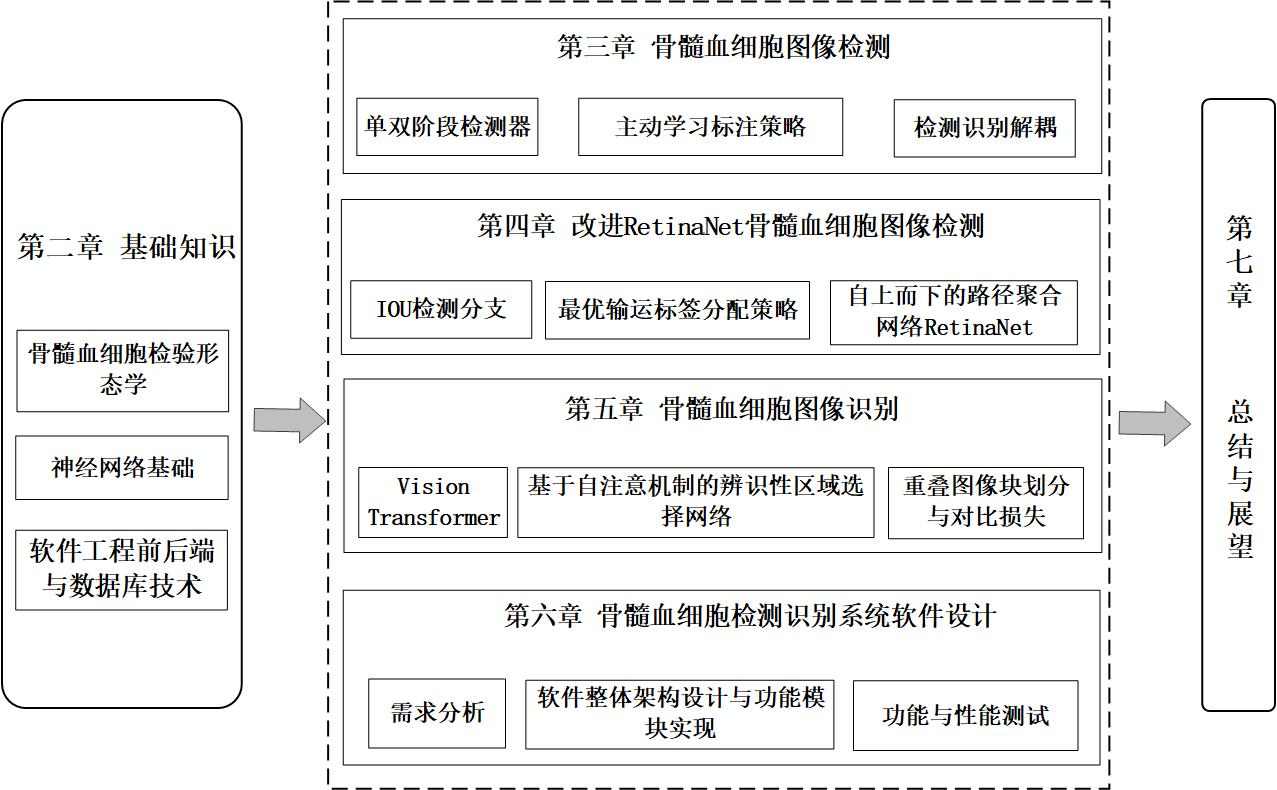
\includegraphics[width=1.0\linewidth]{structure.jpg}
    \caption{论文组织结构}
    \label{fig:structure}
  \end{figure}
  
第一章为绪论。首先介绍了骨髓血细胞形态学检测的背景,并阐述了本文基于深度学习的骨髓血细胞自动化检测与识别的意义。接着,介绍了骨髓血细胞检测与识别的国内外研究现状并
分析各个研究的优势与不足。然后简要说明了本文主要研究内容。最后给出本文的章节组织。

第二章介绍本文的基础知识与技术。本章首先阐述骨髓血细胞相关病理学知识,对比了不同类别骨髓血细胞的形态学差异,介绍骨髓血细胞数据集标注与数据增强方法,并给出了交叉训练集
与测试集的划分。接着,概述神经网络的基本理论与相关检测与识别技术。最后,介绍了软件开发使用的前端、后端与数据库技术。

第三章研究骨髓血细胞检测相关问题。本章对比了多种单阶段与双阶段目标检测网络的检测精度、计算量与速度等性能。并确定将RetinaNet作为为骨髓血细胞检测的基线模型。然后
本章探索了RetinaNet网络在仅检测与检测识别一体化任务上特征提取与识别准确率上的差异,确定了先检测再识别的骨髓血细胞处理流程。

第四章研究基于改进RetinaNet的骨髓血细胞检测网络。针对漏检、误检等问题,在网络结构方面引入了路径聚合网络,缩短底层与顶层特征的信息传递路径,提高网络对
高分辨定位特征的提取能力,减小定位误差。此外引入了引入了IOU预测分支,将检测框的定位质量也纳入到候选框的筛选中。本节对检测网络的标签分配策略进行
研究,提出了一种基于最优输运的全局最优的标签分配策略,提升网络对于血细胞的召回能力与检测精度。

第五章研究骨髓血细胞识别问题。分析了近年来多种基于深度学习的识别网络,提出了一种基于改进Vision Transformer的骨髓血细胞识别模型。
该网络由多个堆叠的自注意编码层组成。为了充分利用自注意力机制,本文采用压缩激发模块学习了多个编码层的注意力权重,该模块可以有效
捕捉到不同细胞之间细微的差异部分,提高网络的细粒度特征表达能力。在训练过程中,将对比损失与交叉熵损失函数进行有机结合,进一步提升网络提取特征的辨识性,该网络模型
在TMAMD骨髓血细胞数据集取得了最佳性能。

第六章介绍骨髓血细胞检测与识别系统软件的设计与实现。本节首先对骨髓血细胞检测识别系统进行需求分析,对软件的开发环境与平台进行说明,
并设计了软件的整体架构。接着详细介绍了数据库表与各个功能模块的设计与实现。最后对软件进行了功能与性能测试,总结了软件的测试结果。

第七章为总结与展望。总结了本文的工作内容,对骨髓血细胞检测与识别的发展进行展望。




% % !TeX root = ../thuthesis-example.tex

\chapter{基础知识}
本章主要介绍本文所涉及的基础理论知识,首先概述了骨髓血细胞不同类别与发育阶段形态学特征。
然后介绍了骨髓血细胞图像数字化与数据集的构建。接着本文介绍了神经网络相关概念,最后对骨髓血细胞检测与识别软件系统涉及到的相关框架进行了介绍。
\section{骨髓血细胞图像及预处理}
\subsection{骨髓血细胞形态学介绍}
人体血细胞主要由骨髓内的造血干细胞分化而成。造血干细胞由髓系干细胞与淋系干细胞构成。其中髓系干细胞分化为粒细胞系统、红细包系统、单核细胞系统与巨核细胞系统,
淋系干细胞分化为浆细胞系统与淋巴细胞系统。不同系统的细胞按照发育成熟过程可以分为原始、早幼与成熟这三个阶段。粒细胞与红细胞的幼稚阶段可再具体划分为早幼,中幼与晚幼这
三个发育阶段。粒细胞系统根据细胞质内特殊颗粒对酸碱性物质亲和性,可分为嗜酸性粒细胞,嗜碱性粒细胞和中性粒细胞。骨髓血细胞六大系统血细胞的发育过程如图~\ref{fig:development}所示:
\begin{figure}
  \centering
  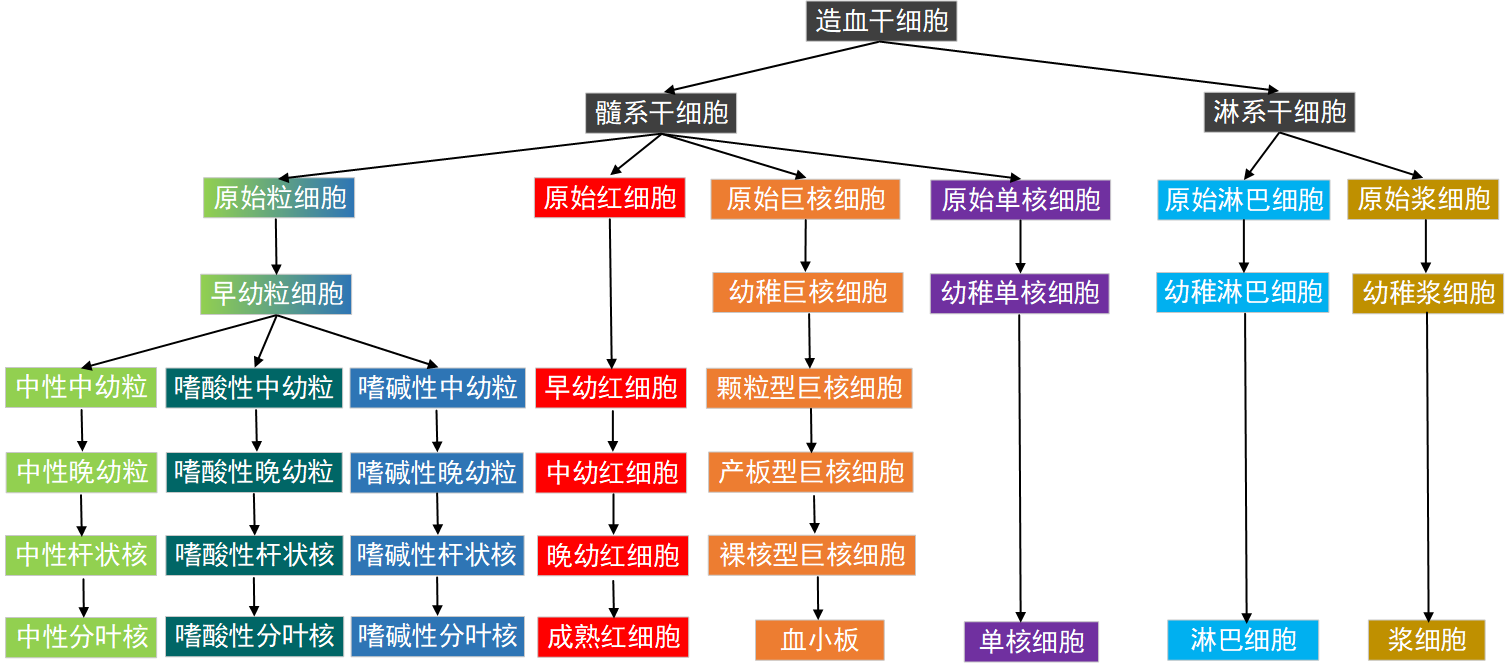
\includegraphics[width=1.0\linewidth]{development.png}
  \caption{骨髓血细胞发育成熟过程示意图}
  \label{fig:development}
\end{figure}

% \begin{itemize}
%   \item 原始细胞:胞体类圆形,直径在10\textasciitilde20微米。细胞核居中,呈圆形,染色质为粗细颗粒状,具有多个小而清晰的核仁。细胞质较少,无颗粒,呈蓝色或深蓝色。
%   \item 单核细胞:胞体呈现圆形或椭圆形,直径在14\textasciitilde25微米。细胞核扭曲折叠,常位于胞体中央或一侧,染色质疏松,核仁消失。细胞质通常为浅灰蓝色,可见空泡与紫红色的粉尘样颗粒。
%   \item 淋巴细胞:胞体为类圆形或不规则,直径在12\textasciitilde15微米。细胞核染色质致密,呈现索块状,形态上存在凹陷或者切迹。细胞质极少,呈现淡蓝色无颗粒。
%   \item 浆细胞:胞体常呈椭圆形或不规则,直径在12\textasciitilde16微米。细胞核多偏位,染色质聚集。细胞质为不透明的深蓝色,在细胞核周有淡染色带。
%   \item 有核红细胞:胞体规则类圆形,直径在7\textasciitilde10微米。细胞核为圆形位于细胞中央,内部含多个紫黑色团块。细胞质较多,无颗粒,为淡红色。
%   \item 早幼粒细胞:胞体较大,圆形或椭圆形,直径在12\textasciitilde25微米。细胞核较大,内部染色质细致,有清晰可见的核仁。细胞质为深蓝色,含有分布不均、形态不一的非特异性颗粒。
%   \item 中性中幼粒细胞:胞体为类圆形,直径在10\textasciitilde20微米。细胞核为半圆形或微凹陷,无核仁,染色质密集索块状。细胞质呈淡蓝色,其中存在大小均一,密集的淡粉红色中性颗粒。
%   \item 中性晚幼粒细胞:胞体类圆形,直径在10\textasciitilde16微米。细胞核呈半月形,存在凹陷,凹陷程度小于直径的1/2。染色质聚集小块状。细胞质多,淡蓝色,存在较多中性颗粒。
%   \item 中性杆状核细胞:胞体类圆形,直径10\textasciitilde15微米。细胞核为杆状、S形、U形等,凹陷程度大于直径的1/2,染色质粗块状。细胞质丰富,淡蓝色,充满中性颗粒。
%   \item 中性分页核细胞:胞体类圆形,直径10\textasciitilde14微米。细胞核通常分为2-5叶,之间通过核丝连接。细胞质丰富含有较多中性颗粒。
%   \item 嗜酸性粒细胞:胞体直径15\textasciitilde20微米。特点类似中性粒细胞,细胞质中存在大小分布均一,橘红色的嗜酸性颗粒。
% \end{itemize}
不同类别的骨髓血细胞胞体形状各异且细胞核与细胞浆会呈现出不同的颜色与纹理特征。表~\ref{table:cell_feature}
对本文主要关注的骨髓血细胞类别进行细胞核、细胞质等形态学方面的简要介绍。
\begin{longtable}{ccccc}
  % \centering
  \caption[Short Caption]{骨髓血细胞形态学特征}
  \label{table:cell_feature} \\
  % 下面是表头
  \hline
  \textbf{细胞名称} & \textbf{图像示例} & \textbf{胞体特征} & \textbf{细胞核} & \textbf{细胞质} \\ 
  \hline 
  \endfirsthead
  % 下面数字3的意思是表格的列数
  \multicolumn{5}{c}%
  {{\tablename\ \thetable{} --接上表}} \\
  \hline 
  \textbf{细胞名称} & \textbf{图像示例} & \textbf{胞体特征} & \textbf{细胞核} & \textbf{细胞质} \\ 
  \hline  
  % 注意这里把表头复制了一遍,因为在新的页面也会展示一下表头,不然表格不方便阅读
  \endhead
  \hline 
  % \multicolumn{5}{r}{{骨髓血细胞形态学特征}} \\ \hline
  \endfoot
  \endlastfoot
  原始细胞 & 
  \multicolumn{1}{m{0.15\textwidth}}{
  \begin{minipage}[b]{0.15\textwidth}
      \centering
      {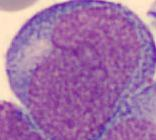
\includegraphics[width=0.9\textwidth]{cell_example/原始细胞.jpg}}
  \end{minipage}} &  
  \multicolumn{1}{m{0.15\textwidth}}{类圆形,直径10\textasciitilde20微米} & 
  \multicolumn{1}{m{0.20\textwidth}}{居中,呈圆形,染色质为颗粒状,具有多个小而清晰的核仁} & 
  \multicolumn{1}{m{0.20\textwidth}}{细胞质较少,无颗粒,呈蓝色或深蓝色}\\
  \midrule[0.5pt]
  单核细胞 & 
  \multicolumn{1}{m{0.15\textwidth}}{
  \begin{minipage}[b]{0.15\textwidth}
      \centering
      {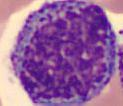
\includegraphics[width=0.9\textwidth]{cell_example/单核细胞.jpg}}
  \end{minipage}} &  
  \multicolumn{1}{m{0.15\textwidth}}{圆形或椭圆形,直径在14\textasciitilde25微米} & 
  \multicolumn{1}{m{0.20\textwidth}}{扭曲折叠,常位于胞体中央或一侧,染色质疏松,核仁消失} & 
  \multicolumn{1}{m{0.20\textwidth}}{通常为浅灰蓝色,可见空泡与紫红色的粉尘样颗粒}\\
  \midrule[0.5pt]
  淋巴细胞 & 
  \multicolumn{1}{m{0.15\textwidth}}{
  \begin{minipage}[b]{0.15\textwidth}
      \centering
      {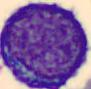
\includegraphics[width=0.9\textwidth]{cell_example/淋巴细胞.jpg}}
  \end{minipage}} &  
  \multicolumn{1}{m{0.15\textwidth}}{类圆形或不规则,直径在12\textasciitilde15微米} & 
  \multicolumn{1}{m{0.20\textwidth}}{染色质致密,呈现索块状,形态上存在凹陷或者切迹} & 
  \multicolumn{1}{m{0.20\textwidth}}{细胞质极少,呈现淡蓝色,无颗粒。}\\
  \midrule[0.5pt]
  浆细胞 & 
  \multicolumn{1}{m{0.15\textwidth}}{
  \begin{minipage}[b]{0.15\textwidth}
      \centering
      {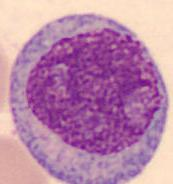
\includegraphics[width=0.9\textwidth]{cell_example/浆细胞.jpg}}
  \end{minipage}} &  
  \multicolumn{1}{m{0.15\textwidth}}{椭圆形或不规则,直径在12\textasciitilde16微米} & 
  \multicolumn{1}{m{0.20\textwidth}}{多偏位,染色质聚集} & 
  \multicolumn{1}{m{0.20\textwidth}}{细胞质为不透明的深蓝色,在细胞核周有淡染色带}\\
  \midrule[0.5pt]
  有核红细胞 & 
  \multicolumn{1}{m{0.15\textwidth}}{
  \begin{minipage}[b]{0.15\textwidth}
      \centering
      {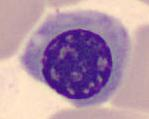
\includegraphics[width=0.9\textwidth]{cell_example/红细胞.jpg}}
  \end{minipage}} &  
  \multicolumn{1}{m{0.15\textwidth}}{规则类圆形,直径在7\textasciitilde10微米} & 
  \multicolumn{1}{m{0.20\textwidth}}{圆形位于细胞中央,内部含多个紫黑色团块} & 
  \multicolumn{1}{m{0.20\textwidth}}{细胞质较多,无颗粒,为淡红色。}\\
  \midrule[0.5pt]
  早幼粒细胞 & 
  \multicolumn{1}{m{0.15\textwidth}}{
  \begin{minipage}[b]{0.15\textwidth}
      \centering
      {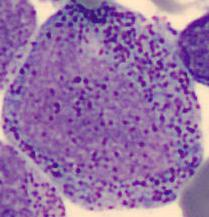
\includegraphics[width=0.9\textwidth]{cell_example/早幼粒细胞.jpg}}
  \end{minipage}} &  
  \multicolumn{1}{m{0.15\textwidth}}{较大,圆形或椭圆形,直径在12\textasciitilde25微米} & 
  \multicolumn{1}{m{0.20\textwidth}}{核较大,内部染色质细致,有清晰可见的核仁} & 
  \multicolumn{1}{m{0.20\textwidth}}{细胞质为深蓝色,含有分布不均、形态不一的非特异性颗粒}\\
  \midrule[0.5pt]
  中性中幼粒细胞 & 
  \multicolumn{1}{m{0.15\textwidth}}{
  \begin{minipage}[b]{0.15\textwidth}
      \centering
      {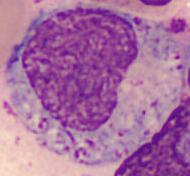
\includegraphics[width=0.9\textwidth]{cell_example/中幼粒细胞.jpg}}
  \end{minipage}} &  
  \multicolumn{1}{m{0.15\textwidth}}{类圆形,直径在10\textasciitilde20微米} & 
  \multicolumn{1}{m{0.20\textwidth}}{半圆形或微凹陷,无核仁,染色质密集索块状} & 
  \multicolumn{1}{m{0.20\textwidth}}{细胞质呈淡蓝色,其中存在大小均一,密集的淡粉红色中性颗粒}\\
  \midrule[0.5pt]
  中性晚幼粒细胞 & 
  \multicolumn{1}{m{0.15\textwidth}}{
  \begin{minipage}[b]{0.15\textwidth}
      \centering
      {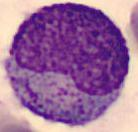
\includegraphics[width=0.9\textwidth]{cell_example/中性晚幼粒.jpg}}
  \end{minipage}} &  
  \multicolumn{1}{m{0.15\textwidth}}{胞体类圆形,直径在10\textasciitilde16微米} & 
  \multicolumn{1}{m{0.20\textwidth}}{呈半月形,存在凹陷,凹陷程度小于直径的1/2,染色质聚集小块状} & 
  \multicolumn{1}{m{0.20\textwidth}}{细胞质多,淡蓝色,存在较多中性颗粒}\\
  \midrule[0.5pt]
  中性晚幼粒细胞 & 
  \multicolumn{1}{m{0.15\textwidth}}{
  \begin{minipage}[b]{0.15\textwidth}
      \centering
      {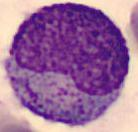
\includegraphics[width=0.9\textwidth]{cell_example/中性晚幼粒.jpg}}
  \end{minipage}} &  
  \multicolumn{1}{m{0.15\textwidth}}{胞体类圆形,直径在10\textasciitilde16微米} & 
  \multicolumn{1}{m{0.20\textwidth}}{呈半月形,存在凹陷,凹陷程度小于直径的1/2,染色质聚集小块状} & 
  \multicolumn{1}{m{0.20\textwidth}}{细胞质多,淡蓝色,存在较多中性颗粒}\\
  \midrule[0.5pt]
  中性杆状核细胞 & 
  \multicolumn{1}{m{0.15\textwidth}}{
  \begin{minipage}[b]{0.15\textwidth}
      \centering
      {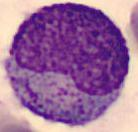
\includegraphics[width=0.9\textwidth]{cell_example/中性晚幼粒.jpg}}
  \end{minipage}} &  
  \multicolumn{1}{m{0.15\textwidth}}{胞体类圆形,直径在10\textasciitilde16微米} & 
  \multicolumn{1}{m{0.20\textwidth}}{呈半月形,存在凹陷,凹陷程度小于直径的1/2,染色质聚集小块状} & 
  \multicolumn{1}{m{0.20\textwidth}}{细胞质多,淡蓝色,存在较多中性颗粒}\\
  \midrule[0.5pt]
  中性分页核细胞 & 
  \multicolumn{1}{m{0.15\textwidth}}{
  \begin{minipage}[b]{0.15\textwidth}
      \centering
      {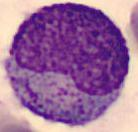
\includegraphics[width=0.9\textwidth]{cell_example/中性晚幼粒.jpg}}
  \end{minipage}} &  
  \multicolumn{1}{m{0.15\textwidth}}{胞体类圆形,直径在10\textasciitilde16微米} & 
  \multicolumn{1}{m{0.20\textwidth}}{呈半月形,存在凹陷,凹陷程度小于直径的1/2,染色质聚集小块状} & 
  \multicolumn{1}{m{0.20\textwidth}}{细胞质多,淡蓝色,存在较多中性颗粒}\\
  \midrule[0.5pt]
  嗜酸性粒细胞 & 
  \multicolumn{1}{m{0.15\textwidth}}{
  \begin{minipage}[b]{0.15\textwidth}
      \centering
      {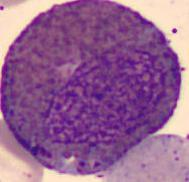
\includegraphics[width=0.9\textwidth]{cell_example/嗜酸性.jpg}}
  \end{minipage}} &  
  \multicolumn{1}{m{0.15\textwidth}}{直径15\textasciitilde20微米。} & 
  \multicolumn{1}{m{0.20\textwidth}}{类似中性粒细胞,染色质聚集索块} & 
  \multicolumn{1}{m{0.20\textwidth}}{大小分布均一,橘红色的嗜酸性颗粒}\\
  \midrule[0.5pt]
  嗜碱性粒细胞 & 
  \multicolumn{1}{m{0.15\textwidth}}{
  \begin{minipage}[b]{0.15\textwidth}
      \centering
      {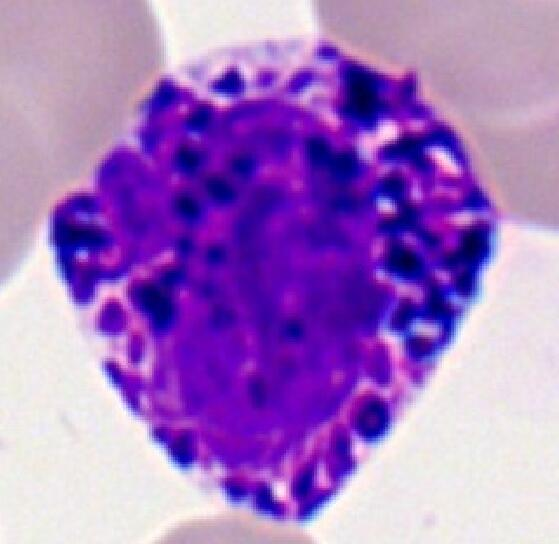
\includegraphics[width=0.9\textwidth]{cell_example/嗜碱性.jpg}}
  \end{minipage}} &  
  \multicolumn{1}{m{0.15\textwidth}}{直径10\textasciitilde15微米。} & 
  \multicolumn{1}{m{0.20\textwidth}}{染色质细致} & 
  \multicolumn{1}{m{0.20\textwidth}}{颗粒粗大,大小形态不一深紫红色的颗粒,部分颗粒覆盖在细胞核上}\\
  \bottomrule[1.5pt]
  \end{longtable}
\subsection{骨髓血细胞数据集与预处理}

\textbf{1)骨髓血细胞切片与数字化}

骨髓血细胞形态学检验技术是临床诊断血液疾病的重要依据。该过程由取材、制片、固定、染色、洗涤干燥与镜检等流程组成。首先通过骨髓穿刺采集骨髓液样本。接着将骨髓液
置于载玻片上制作成薄厚均一的涂片。在涂片制作完成后,使用甲醛或乙醇溶液将其固定。然后采用瑞特-吉姆萨染色剂进行适当时间的着色,染色完成后使用清水冲洗,待自然风干后以备观察。
最后使用光学显微镜对骨髓涂片进行观察,统计骨髓中不同类型血细胞的数量、比例,形态以及是否存在异常细胞,进行骨髓评估判断病情。具体如图~\ref{fig:cell_pre}所示:

\begin{figure}[htbp]
	\centering
	\begin{subfigure}{0.325\linewidth}
		\centering
		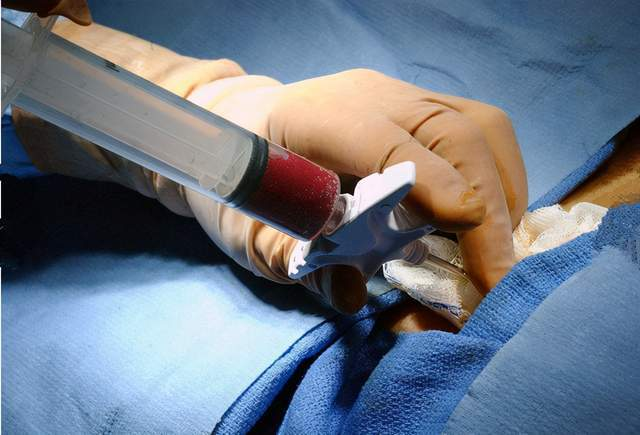
\includegraphics[width=0.95\linewidth, height=0.7\linewidth]{cell_pre/step1.jpg}
    \caption{}
	\end{subfigure}
	\centering
	\begin{subfigure}{0.325\linewidth}
		\centering
		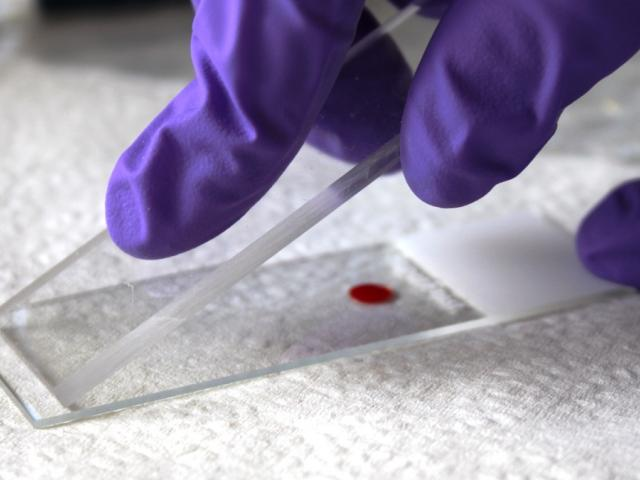
\includegraphics[width=0.95\linewidth, height=0.7\linewidth]{cell_pre/step2.jpg}
    \caption{}
	\end{subfigure}
	\centering
	\begin{subfigure}{0.325\linewidth}
		\centering
		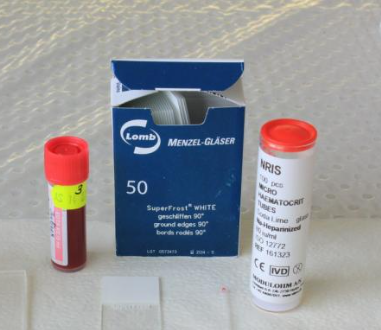
\includegraphics[width=0.95\linewidth, height=0.7\linewidth]{cell_pre/step3.jpg}
    \caption{}
	\end{subfigure}

	\centering
	\begin{subfigure}{0.325\linewidth}
		\centering
		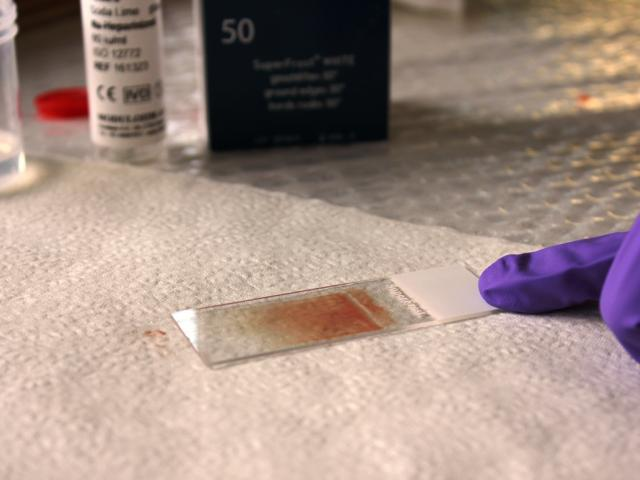
\includegraphics[width=0.95\linewidth, height=0.7\linewidth]{cell_pre/step4.jpg}
    \caption{}
	\end{subfigure}
	\centering
	\begin{subfigure}{0.325\linewidth}
		\centering
		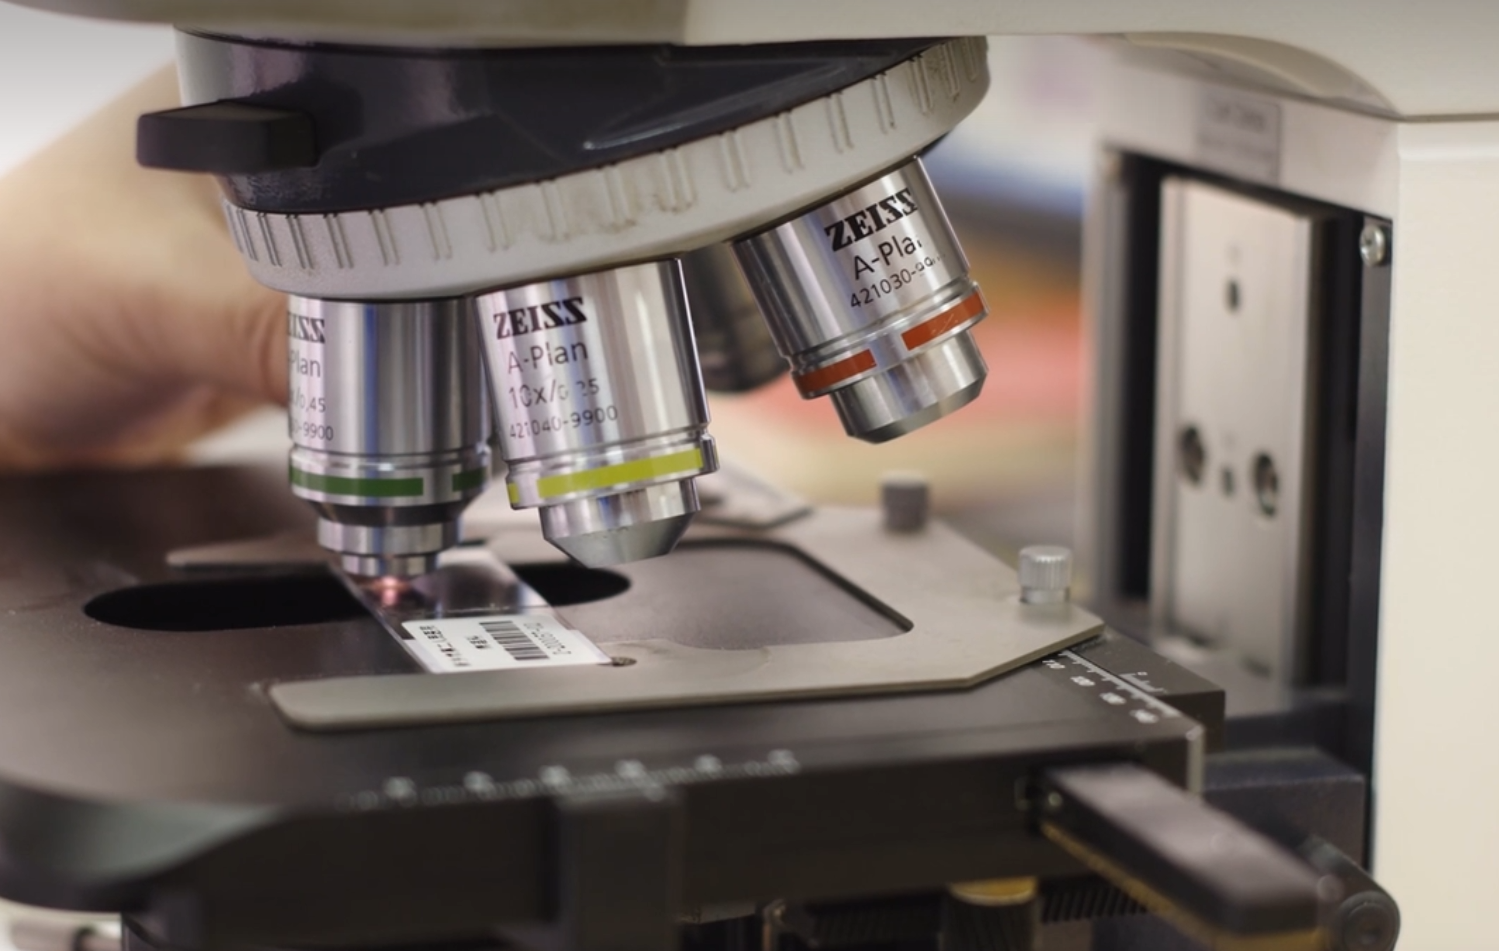
\includegraphics[width=0.95\linewidth, height=0.7\linewidth]{cell_pre/step5.jpg}
    \caption{}
	\end{subfigure}
	\centering
	\begin{subfigure}{0.325\linewidth}
		\centering
		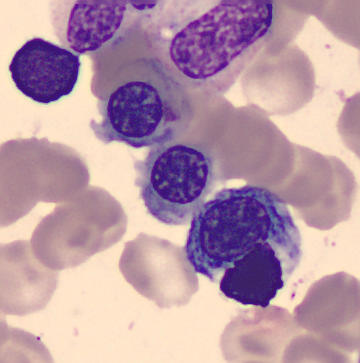
\includegraphics[width=0.95\linewidth, height=0.7\linewidth]{cell_pre/step6.jpg}
    \caption{}
	\end{subfigure}
	\caption{骨髓血细胞检验技术流程:(a)骨髓穿刺抽取骨髓液,(b)制备骨髓涂片,(c)瑞特-吉姆萨染色,(d)清洗晾干,(e)人工镜检判读,(f)骨髓形态学图片}
	\label{fig:cell_pre}
\end{figure}

对骨髓血细胞切片图像进行自动化评估分析首先需要对切片图像进行数字化,从而可以在计算机上进行存储,传输与分析。数字化技术可以为医学研究提供大量数据源,
促进医学研究与临床实验,方便医生进行更加快速与精准的病情分析。病理图像数字化技术由以下几个步骤组成。1)数字扫描:对制备好的组织切片使用数字成像与扫描设备生成数字图像,
一般通过CCD相机采用对焦深度法自动获取对焦位置并扫描成像。2)数字化处理:对图像进行去噪、分割与边缘检测等进一步提升图像质量。3)云存储与管理,将数字化图像存储在
云端服务器中,保证数据的完整性与安全。4)数字分析与诊断,利用计算机视觉等深度学习图像分析技术,对数字化后的病理图像进行分析与诊断,提高病理诊断的效率与准确性。

\textbf{2)数据集标注}

本文使用数据来源于实践基地邃蓝智能科技有限公司合作医院提供的脱敏数据。
数据标注是深度学习模型训练的基础,并且直接影响模型的性能和泛化能力。我们在合作医院病理医师的协作下对血细胞的边界框与类别信息进行精准的标注,完成了骨髓血细胞数据集(BMCD, Bone Marrow Cell Dataset)的制作。
原始数据集总共包含9250张骨髓血细胞图像,我们只关注图像中的有核细胞,而将成熟红细胞作为背景。因为缺少相关专业知识,我们仅标记出血细胞边界框的位置。
我们使用labelme软件作为标注工具,如图~\ref{fig:annotations}所示,针对每一张图像生成json标注文件,记录血细胞边界框的左上角与右下角的坐标,最后再将标注转化为coco格式,并将数据集划分为训练集、测试集与验证集。
经过检测网络,我们得到了单一血细胞图像,即图像中仅有一个完整的骨髓血细胞,这些图像再由经验丰富的病理医生完成类别标签的标注。


\begin{figure}
  \centering
  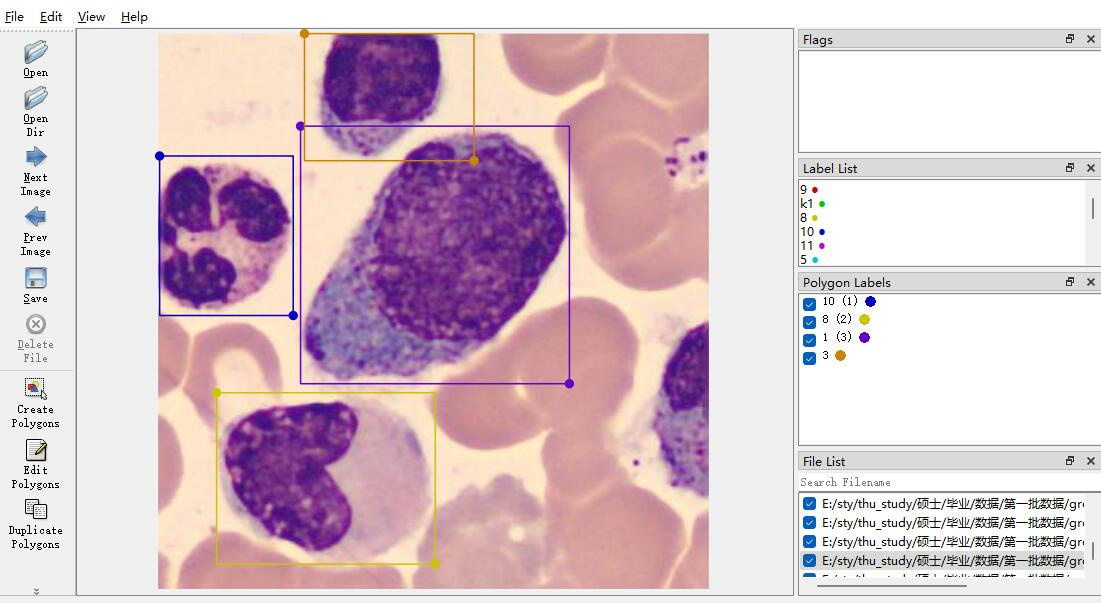
\includegraphics[width=0.8\linewidth]{annotations.jpg}
  \caption{labelme标注软件工具}
  \label{fig:annotations}
\end{figure}

大量的数据标注需要消耗很高的人力物力成本,我们采用主动学习技术去发掘数据集中高信息量的样本,提高标注的效率与精度,降低标注成本。
主动学习的基本思想是标注少量部分数据,利用已标注的数据训练深度学习模型。然后使用模型对未标注的数据进行预测,根据最大化熵、不确定度采样等进行排序,
筛选出不确定性最高的一些数据优先进行标注。不断迭代上述过程,直到标注与模型性能达到预期。具体而言,对于血细胞检测任务,首先标注将部分图像,然后训练Faster-RCNN网络
得到一个初步的检测模型,然后对每张图像进行检测,并生成标注json文件,再反馈到labelme标注软件中进行微调。针对血细胞识别任务,经过检测网络,我们得到了多张单个血细胞图像,首先完成部分
类别标注,训练初步的识别网络。对未标注的血细胞筛选出熵最大的预测样本反馈给病理医生进行核对。主动学习流程如图~\ref{fig:active}所示:

\begin{figure}
  \centering
  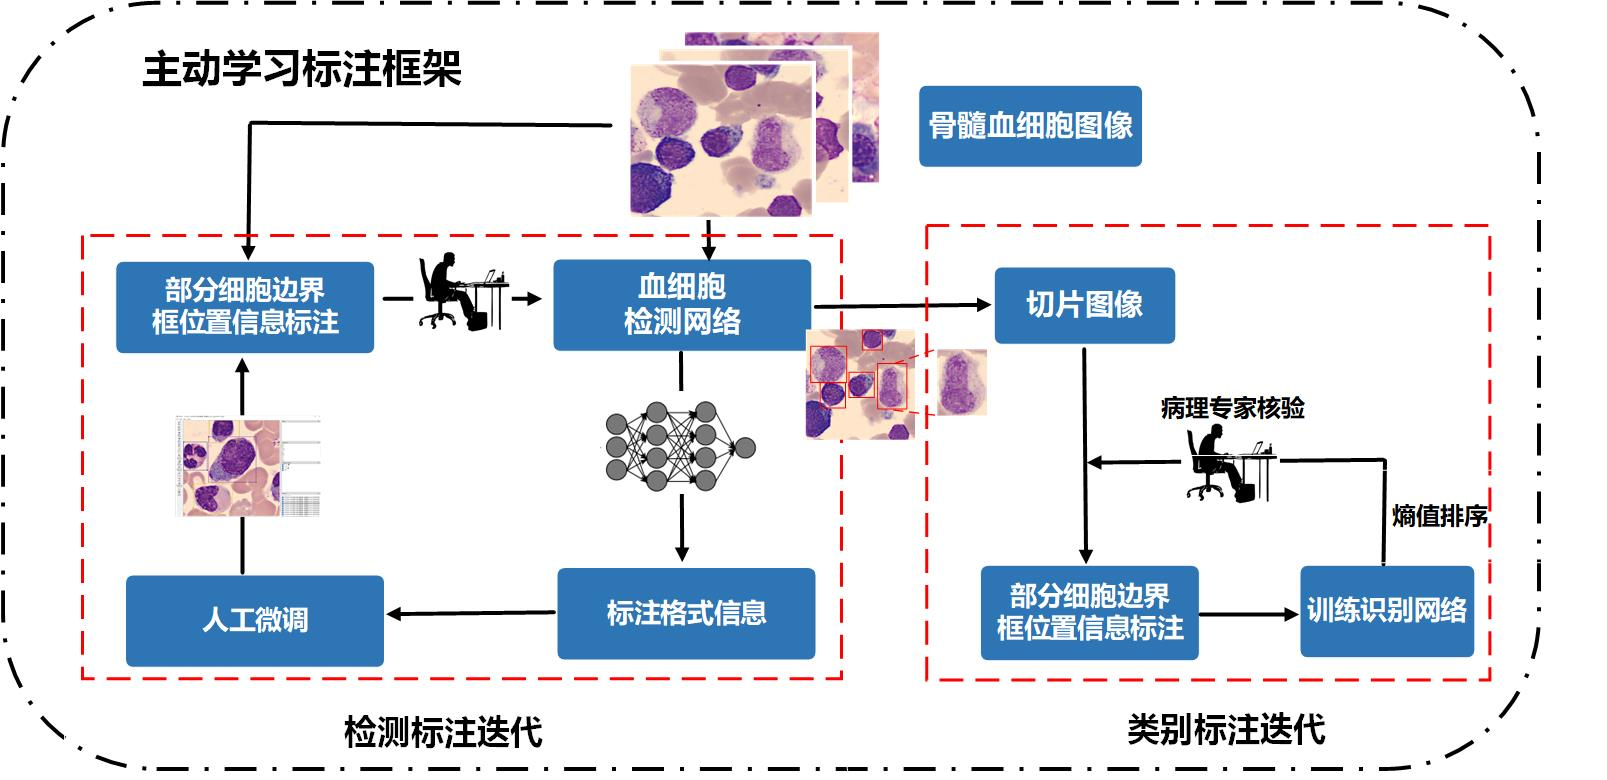
\includegraphics[width=1.0\linewidth]{active.jpg}
  \caption{主动学习标注框架示意图}
  \label{fig:active}
\end{figure}
\textbf{3)数据增强}

我们主要关注的五大系统细胞在人体内占比不同,粒细胞系统约占全部细胞的50\%,而浆细胞系统一般占比小于1.5\%,由于细胞天然就存在比例不均衡问题,其也导致了我们的数据集
存在严重的类别不平衡问题。例如单核细胞数量仅为有核红细胞数量的1/9。数据的不平衡会导致网络过多的关注数量较多的类别特征信息,数量较少类别易出现准确率与召回率的不均衡,影响模型的泛化性能。
为解决上述问题,本文对于数量较多的类别采用随机欠采样减少样本数量。对于数量较少的类别,采用翻转、旋转、添加噪声与色彩调整增加数据多样性。下面对数据增强方法进行简要介绍:
1)翻转:将图像沿水平或垂直方向进行镜像对称,生成新的图像。当图像$I(x,y)$沿水平方向进行翻转后,水平翻转图像为$I’(x, y)=I(w-x-1,y)$,其中w为原始图像宽度。
2)旋转:将图像沿着某个点或轴进行旋转,当图像$I(x,y)$以$(c_x, c_y)$为旋转中心时,旋转角度为$\theta$, 旋转后的图像为$I’(x, y)=I((x - c_x)\cos\theta - (y - c_y)\sin\theta + c_x, (x - c_x)\sin\theta - (y - c_y)\cos\theta + c_y)$。
3)添加噪声:常用的图像噪声包括高斯噪声、椒盐噪声与泊松噪声。高斯噪声是一种连续随机噪声,服从零均值、标准差为$\sigma$的正态分布,会使得图像变模糊。
椒盐噪声是离散随机噪声,图像中会出现亮点与暗点,降低图像的清晰度与对比。
4)色彩调整:常用方法包括了亮度调整、对比度调整、色相调整与饱和度调整。

\section{神经网络技术概述}
\subsection{神经元与梯度优化}

\textbf{1)神经元}

神经网络发展历史最早可以追溯到20世纪五十年代,当时研究人员受到神经科学启发,模拟生物神经元结构提出了神经网络。
神经元是神经网络的基本单元,其结构如图~\ref{fig:neuron}所示,由输入、加权、激活函数、输出这四个部分组成。
\begin{figure}
  \centering
  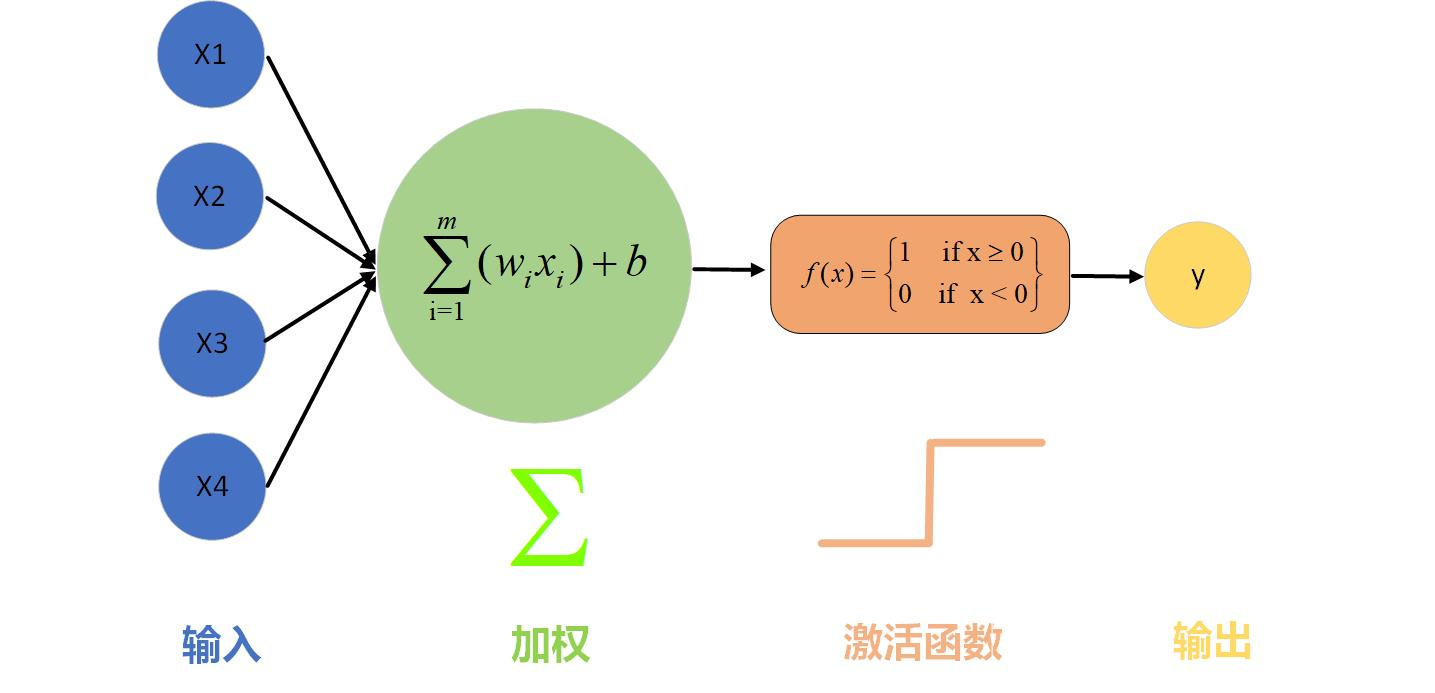
\includegraphics[width=0.8\linewidth]{neuron.jpg}
  \caption{神经元结构示意图}
  \label{fig:neuron}
\end{figure}

输入部分,神经元接收其他神经元的信息$x_1, x_2, \dots, x_4$,每个输入与权重进行关联。加权部分表示神经元对于输入部分的敏感程度。
激活函数将加权和进行变换,保证输出数值范围并引入非线性的特性。输出部分是激活函数处理后的结果,如式~\ref{eq:neuron}所示,可作为后续神经元的输入。

\begin{equation}
  h(x) = f({{\bf{W}}^T}{\bf{x}}) = f(\sum\limits_{i = 1}^m {{w_i}{x_i} + b})
  \label{eq:neuron}
\end{equation}

式~\ref{eq:neuron}中$f(\cdot)$为激活函数。常用的激活函数有修正线性单元函数(Rectified linear unit function,ReLU)、双曲正切函数、sigmoid函数等。

\textbf{2)感知机}

感知机由美国心理学家弗兰克·罗森布\cite{1958perceptron}在1958年提出,它是一种最简单的神经网络,拓扑结构如图~\ref{fig:perceptron}所示。
网络包含了输入层、隐含层与输出层,前一层的每个神经元都与后一层的神经元相连。前一层神经元输出信息传递到下一层神经元的过程称为前向传播。
该过程可以用一系列矩阵乘法与激活函数进行描述,若输入数据为$x$, 网络结构总共有$L$层,则前向传播过程可以表示为:

\begin{equation}
  \begin{aligned}
  z^{1} & =W^{1} x+b^{1} \\
  a^{1} & =g^{1}\left(z^{1}\right) \\
  & \vdots \\
  z^{L} & =W^{L} a^{L-1}+b^{L} \\
  a^{L} & =g^{L}\left(z^{L}\right)=\hat{y}
  \label{eq:perceptron}
\end{aligned}
\end{equation}

其中 $z^{l}$ 表示第$l$层的未激活值,$a^{l}$ 表示第$l$层的激活值,$W^{l}$ 和 $b^{l}$ 分别表示第$l$层的权重矩阵和偏置向量。
\begin{figure}
  \centering
  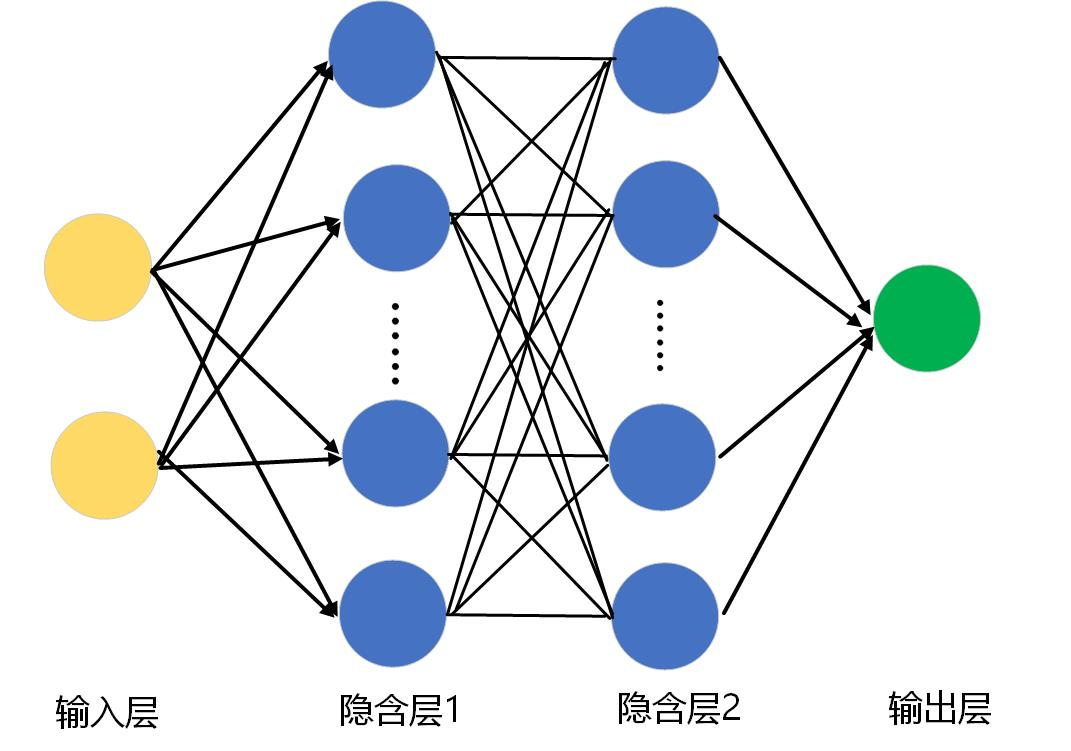
\includegraphics[width=0.65\linewidth]{perceptron.jpg}
  \caption{感知机网络模型示意图}
  \label{fig:perceptron}
\end{figure}

\textbf{3)反向传播与梯度优化}

反向传播全称是误差反向传播(back propgation,BP),是用于神经网络训练的算法。神经网络经过前向传播得到网络预测值,采用
损失函数衡量预测值与真实值之间的误差。通过损失函数最小化计算神经网络参数的导数,然后调整更新神经网络权重参数以减小误差。不断迭代上述过程,
直到模型参数收敛。

假设 $L$ 为损失函数,$w_{ij}^k$ 表示第$k$层第$i$个神经元到第$j$个神经元之间的权重,$a_j^l$ 表示$l$ 层的第$j$个神经元的非激活值
$z_j$ 表示第 $j$ 层神经元输出,$\sigma_l(\cdot)$为第l层激活函数。反向传播过程计算过程如下:
\begin{enumerate}[label=(\alph*)]
  \item 网络进行前向传播得到预测值
  \item 定义输出层的误差$\delta_k^L$为损失函数对输出层非激活值的导数,如式~\ref{eq:delta}所示,
  \begin{equation}
    \delta_k^L = \frac{\partial L}{\partial a_k^L} = \frac{\partial L}{\partial z_k^L} \frac{\partial z_k^L}{\partial a_k^L}
    \label{eq:delta}
  \end{equation}
  \item 对于中间隐含层,可以通过链式法则求出第$l$层的传播误差$\delta_j^l$
  \begin{equation}
    \begin{aligned}
    \delta_j^l & = \frac{\partial L}{\partial a_j^l} = \frac{\partial L}{\partial z_j^l} \frac{\partial z_j^l}{\partial a_j^l} \\
    \frac{{\partial L}}{{\partial z_j^l}} & = \sum\limits_i^{} {\frac{{\partial L}}{{\partial a_i^{l + 1}}}} \frac{{\partial a_i^{l + 1}}}{{\partial z_j^l}} = \sum\limits_i^{} {\delta _i^{l + 1}} w_{ij}^{l + 1} \\
    \delta_j^l & = \frac{{\partial L}}{{\partial a_j^l}} = \sigma _l^\prime \left( {a_j^l} \right)\sum\limits_i^{} {w_{ij}^{l + 1}} \delta _i^{l + 1}
    \end{aligned}
    \label{eq:delta_l}
  \end{equation}
  \item 计算损失函数对于某一隐含层$l$权重$w_{ij}^k$的梯度值
  \begin{equation}
    \frac{{\partial L}}{{\partial w_{ij}^l}} = \frac{{\partial L}}{{\partial a_j^l}}\frac{{\partial a_j^l}}{{\partial w_{ij}^l}} = \delta_j^l z_i^{l - 1}
    \label{eq:delta_w}
  \end{equation}
  \item 若训练的学习率为$\eta$,随机抽取小批量样本$\left\{ {\left( {{{\bf{x}}_m},{{\bf{y}}_m}} \right)} \right\}_{m = 1}^{{N_0}}$,权重值的更新如下
  \begin{equation}
    w_{ij}^{l(\tau  + 1)} = w_{ij}^{l(\tau )} - \eta \frac{1}{{{N_0}}}\sum\limits_{m = 1}^{{N_0}} {\frac{{\partial {L_m}}}{{\partial w_{ij}^l}}}
    \label{eq:update}
  \end{equation}
  \item 重复上述步骤,直到损失函数达到极小值,得到收敛后最优的网络模型参数
\end{enumerate}

\textbf{4)优化算法}

在定义好损失函数后,通过误差反向传播算法调整网络中的权重参数,使得网络在训练数据集上的误差最小化。但传统梯度优化算法面临着诸多困难,
损失函数存在着大量的鞍点与平坦区域,可能收敛到局部极小值点。此外训练集数据量巨大,计算全部数据梯度非常耗时。针对上述问题,研究学者提出了小批量
随机梯度下降算法(mini-batch stochastic gradient descent),每次从训练集中随机抽取出m个样本组成小批量样本,对于这组样本计算梯度均值用于更新权重系数,如式~\ref{eq:msgd}所示

\begin{equation}
  \begin{aligned}
    \boldsymbol{g}  & \leftarrow \nabla_{w}\left(\frac{1}{m} \sum_{i=1}^{m} L\left(f\left(\boldsymbol{x}_{i} ; \boldsymbol{w}\right), \boldsymbol{y}_{i}\right)\right) \\
    \boldsymbol{w}  & \leftarrow  \boldsymbol{w} - \eta \boldsymbol{g}
  \end{aligned}
  \label{eq:msgd}
\end{equation}

小批量随机梯度下降算法面临着学习率选择困难问题。学习率过小收敛慢,过大导致震荡。Adagrad是最早的自适应学习率优化算法。
其设置了一个梯度二阶累积统计量$r$,每次使用小批量梯度平方和来更新$r$,权重更新如下

\begin{equation}
  \begin{aligned}
    \boldsymbol{r}  & \leftarrow   \boldsymbol{r}  +  \boldsymbol{g}^2\\
    \boldsymbol{w}  & \leftarrow  \boldsymbol{w} - \frac{\eta}{\sqrt{r + \delta}} \boldsymbol{g}
  \end{aligned}
  \label{eq:adagrad}
\end{equation}

Adagrad算法在训练后期,由于累计平方很大,网络更新停止。针对上述问题,RMSProp优化算法设置了一个衰减系数$\rho$,r的更新公式如下:
\begin{equation}
  \begin{aligned}
    \boldsymbol{r}  & \leftarrow  \rho \boldsymbol{r}  + (1-\rho) \boldsymbol{g}^2\\
  \end{aligned}
  \label{eq:Rmsprop}
\end{equation}

Adam优化算法(Adaptive Moment estimation)集成了动量与多种优化算法的优势,使梯度更新更平滑,适用于大多数的神经网络优化问题,是目前应用最广泛的梯度优化算法。
该算法计算了梯度的一阶矩$\boldsymbol{m}$与二阶矩$\boldsymbol{v}$,一阶矩类似于动量,降低梯度随机变化大的影响,二阶矩用于控制自适应学习率。参数更新公式如下:

\begin{equation}
  \begin{aligned}
    \boldsymbol{m_t}  & \leftarrow  \beta_1 \boldsymbol{m_{t-1}}  + (1 - \beta_1) \boldsymbol{g_t} \\
    \boldsymbol{v_t}  & \leftarrow  \beta_2 \boldsymbol{v_{t-1}}  + (1 - \beta_2) \boldsymbol{g_t^2} \\
    \boldsymbol{\hat{m_t}} &  \leftarrow \frac{\boldsymbol{m_t}}{1 - \beta_1} \\
    \boldsymbol{\hat{v_t}} &  \leftarrow \frac{\boldsymbol{v_t}}{1 - \beta_2} \\
    \boldsymbol{w}  & \leftarrow  \boldsymbol{w} - \frac{\eta}{\sqrt{\boldsymbol{\hat{v_t}} + \delta}} \boldsymbol{\hat{m_t}}
  \end{aligned}
  \label{eq:Adam}
\end{equation}




\subsection{卷积神经网络}

\textbf{1)基本概念与结构}

卷积神经网络(Convolutional Neural Network, CNN)是计算机视觉领域应用最广泛的神经网络。相比于传统的全连接神经网络,
CNN引入了卷积层与池化层,通过稀疏连接与权值共享,可以更加有效的提取空间数据的特征模式,降低了模型参数量与计算复杂度。
卷积神经网络由多个卷积层、池化层、全连接层等组成,典型结构如图~\ref{fig:cnn}所示。

\begin{figure}
  \centering
  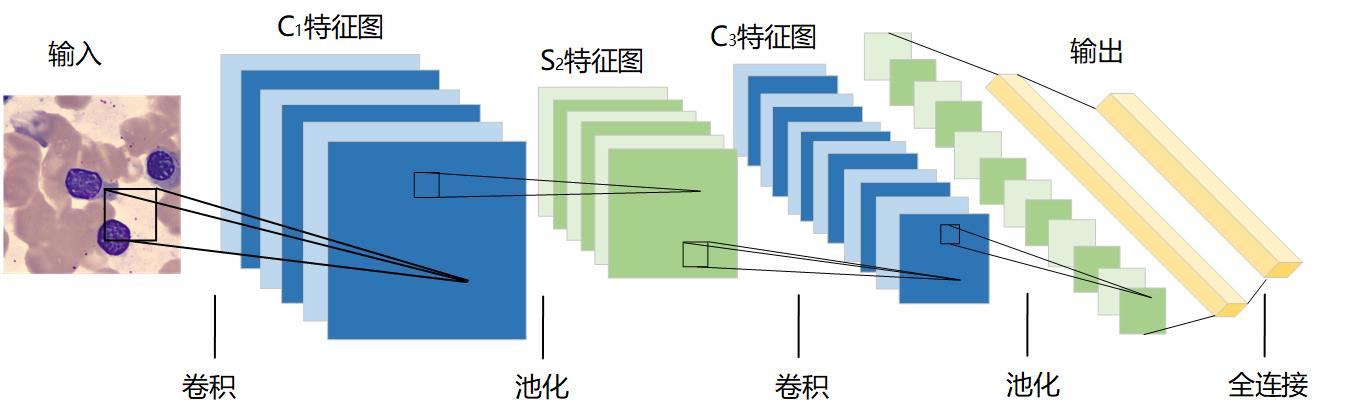
\includegraphics[width=1.0\linewidth]{cnn.jpg}
  \caption{典型卷积神经网络结构示意图}
  \label{fig:cnn}
\end{figure}

\textbf{2)卷积层}

卷积层是卷积神经网络的基础结构。卷积层由多个卷积核构成,每个卷积核用于抽取不同的图像特征,输出一个卷积通道特征。
如图\ref{fig:conv}所示,输入特征图有三个通道,该卷积层有四个卷积核,最终输出包含四个通道的特征图。
多个卷积通道拼接后组成卷积层的输出。卷积核将输入特征图局部区域像素与卷积核对应元素相乘后求和,再将结果写入到输出特征图对应位置,如式~\ref{eq:conv}所示。
卷积核有四个描述参数,卷积核大小(kernel size)、步幅(stride)、边界扩充(stride)、输入与输出通道数量(channel)。
通过卷积操作抽取图像特征,再不断将特征进行组合,形成最终图像的特征描述。

\begin{equation}
  \begin{array}{l}
    y(m, n)=\sum_{i} \sum_{j} I(i, j) h(m-i, n-j) \\
    =\sum \sum I(m-i, n-j) h(i, j)
    \end{array}
  \label{eq:conv}
\end{equation}

卷积核大小为卷积核的宽度与高度,通常小卷积核来提取边缘、线条等纹理特征,大卷积核提取高级抽象特征。步幅控制
卷积核在图像上滑动的距离,决定了输出特征图的大小。步幅增大使得特征图大小减小,从而降低网络的计算复杂度。
边界扩充是图像边界上进行零填充,可以使得图像边缘像素作为卷积核的中心进行卷积,避免边缘信息丢失。卷积核的输入通道数量由
输入特征图的通道数决定。输出通道数据量为卷积核的个数,提高卷积核数量可以增加提取特征的丰富性,从而比高网络的表达能力。

\begin{figure}
  \centering
  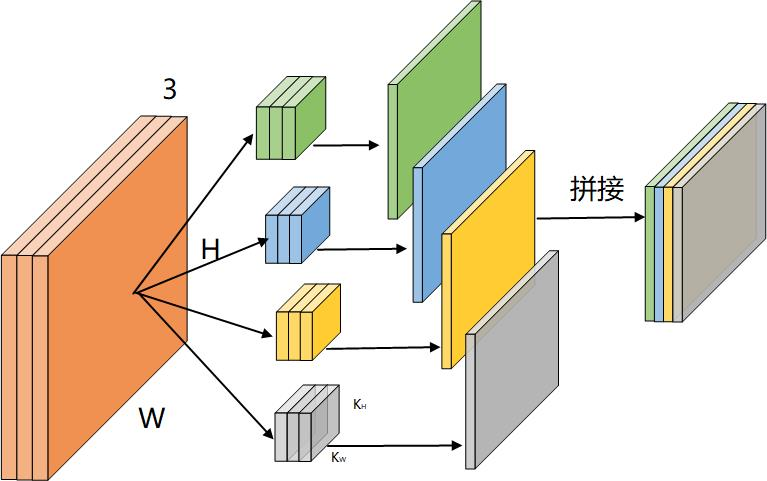
\includegraphics[width=0.7\linewidth]{conv.jpg}
  \caption{CNN卷积层示意图}
  \label{fig:conv}
\end{figure}

\textbf{3)池化层}

池化层位于卷积层后,池化也称为降采样,主要用于特征选择与降维,降低特征图大小,从而降低后续卷积等操作的计算量,
同时能够让网络学习图像有效特征,提高网络的铝棒性与泛化性,避免过拟合问题。
池化操作通过池化核来完成,池化核在图像局部区域内进行下采样,用一个值代表当前区域特性。然后根据步长在图像上从左向右,从上到下滑动。
常用的池化方式有最大池化与平均池化,最大池化在特征图局部区域中选择最大值来表征此区域,最大池化可以使得特征图对比更加显著。
平均池化在局部区域特征图中使用均值来表征此区域,整体特征信息更加平滑。
通常池化核大小选择为$2 \times 2$,然后将输入特征图划分为多个相同大小的区域,以最大池化的方式进行。

\begin{figure}
  \centering
  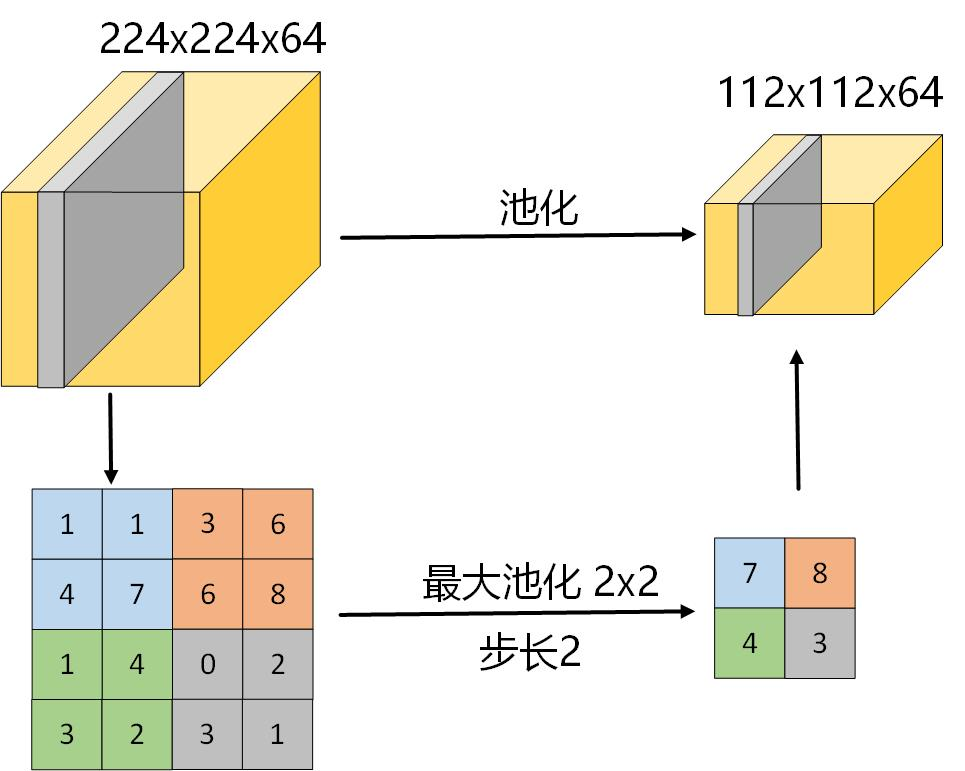
\includegraphics[width=0.6\linewidth]{pool.jpg}
  \caption{CNN池化层示意图}
  \label{fig:pool}
\end{figure}


\section{软件开发相关技术}
本节主要介绍骨髓血细胞检测与识别软件开发使用的技术框架。首先介绍前端核心技术,Vue框架与Element UI组件库。
然后介绍后端使用的框架Django与深度学习模型部署工具ONNX。最后介绍了软件使用的数据库Mysql。

\subsection{前端技术}

前端技术主要用来构建优美的用户图像界面、并提供良好的用户交互。随着互联网技术的飞速发展,前端web技术已经步入到
2.0时代。无论是在移动端还是PC端,我们都能体验到设计精妙绝伦的界面,并进行丰富多元的交互,极大提升了用户的浏览
效率与用户体验。前端开发的三个核心基础要素是超文本标记语言HTML、层叠样式表与Javascript语言。目前,随着前端技术的不断
发展,已存在多种前端框架与组件库工具,可以帮助开发人员可以快速搭建出风格优美统一的界面,提升开发效率。本小结对软件开发
使用到的前端框架与组件库进行简要介绍:

\textbf{1)HTML、CSS与Javascript}

HTML的全称是超文本标记语言(Hypertext Markup Language),是用来构建和布局界面内容的描述语言。该语言使用标签结构与属性标记
对文字、图像、视频、超链接、表格等内容进行不同形式的呈现。目前HTML主要遵循HTML5规范,该版本引入了更多种类的标签、使得界面结构更加清晰。
此外引入了更多的新表单控件。支持多种音频、视频等多媒体形式,无需三方插件。在性能方面也使用了多线程通信与缓存技术,可以更加快速的访问资源
与处理请求。

CSS的全称是层叠样式表(Cascading Style Sheets),它是一种样式表语言,主要用来定义HTML元素的表现形式。通过CSS可以对于页面上的元素
进行精确的布局描述,并为元素添加圆角、阴影、动画或者复杂的过度效果。此外CSS可以根据设备屏幕大小与分辨率对页面的布局和样式进行响应以适应不同的设备。

Javascript是一种解释型的轻量级Web开发编程语言,作为编程代码嵌入到HTML页面后,可以由浏览器进行解释执行。通过javascript语言可以
实现动态效果与用户的交互,例如用户提交表单验证、响应用户的请求、动态界面等。
通过上述三种技术来构建内容,设计样式与行为控制,开发者可以快捷、高效、灵活的创建出更好用户图形界面应用。

\textbf{2)VUE前端框架}

随着前端功能越来越复杂,出现了多种前端框架来简化前端编程开发。JQuery是最早的前端框架,对javascript进行了多种封装,可以更加便捷的操作文档对象模型(Document Object Model)。
在JQuery的基础上演化出MVC架构,即模型(Model)-视图(View)-控制器(Controller)的架构。该架构将界面、数据业务逻辑、信息输入更新进行分离,
使得代码易于维护与升级。目前主流的前端架构是MVVM架构,如图~\ref{fig:mvvm}所示,MVVM是模型(Model)-视图(View)-视图模型(ViewModel)的缩写。模型代表
软件应用的数据模型与业务逻辑。视图是用户界面,将数据可视化呈现。ViewModel监听模型数据改变并控制视图行为,它通过数据的双向绑定将模型与视图连接起来,模型中的变化会
自动同步到视图中,视图中的变化也同步到模型中。Vue.js是一款轻量级、渐进式的MVVM前端框架。相比于其他框架拥有如下的优势:双向数据绑定,避免操作DOM,易于维护;
组件化,将界面拆分为多种组件,每个组件拥有自己的view与model,代码复用性与模型化程度更高;响应式设计,采用虚拟DOM与Diff算法优化渲染效率,极大减少了修改DOM元素的次数;
生态环境丰富,Vue有大量的插件,方便扩展,社区活跃,大量优秀的开发者在持续的对框架进行维护、更新与完善。

\begin{figure}
  \centering
  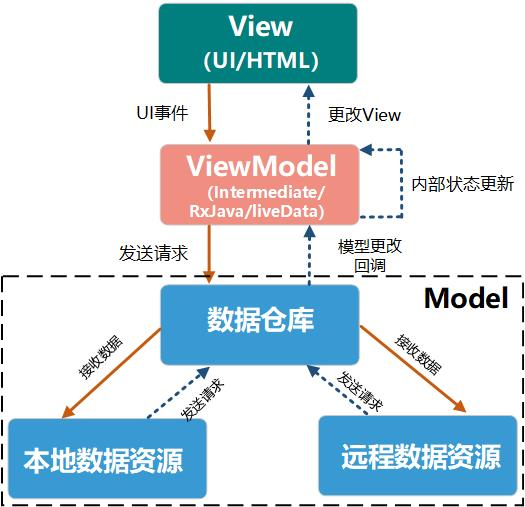
\includegraphics[width=0.7\linewidth]{MVVM.jpg}
  \caption{MVVM框架示意图}
  \label{fig:mvvm}
\end{figure}

\textbf{3)Element-UI组件库}

Element-UI是一套基于Vue 2.0的桌面端组件库,提供了一系列开箱即用的精美UI组件,如表单、布局、弹窗、导航、数据展示等多种组件。这些组件的设计简洁、优美、风格统一,可以帮助开发人员 
高效快速的构建美观、易用的界面程序。Element-UI提供的API接口简单易学,可以轻松的自定义组件扩展。该组件库使用了虚拟滚动技术,极大的提高了页面的渲染性能。

\subsection{后端技术}

\textbf{1)后端框架}

在计算机领域,框架是指一套规范、标准、结构完整的程序模版。框架通常包含了一系列的库、工具与接口,开发者可以按照框架的规范快速进行应用程序开发,
减少重复工作,提高开发效率同时保障软件的可靠性。目前各个编程语言均有自己的Web后端框架,这些框架各具特色,一些框架亮点在分布式、高性能,一些框架优势在与高成熟与高扩展度。

在诸多的编程语言中,Python是一种解释型、面向对象的高级程序设计语言。其优势在于拥有丰富的标准库、框架与详细的官方文档,并且可以方便的跨平台运行。
Python语言被广泛应用在多种领域如数据分析、人工智能、后端开发。在深度学习领域,Pytorch是由Facebook开发的基于Python的开源深度学习框架,在学术界与工业界广泛使用。
本文使用Pytorch框架进行模型训练。

Django是一个基于Python开源的Web后端框架。它最早由Adrian Holovaty和Simon Willison在2003年开发,用于维护劳伦斯集团旗下的
几个新闻网页。该框架于2005年7月在BSD许可证下发布,截至目前,Django已经经历过三个大版本的迭代。最新的Django 3.0版本于2019年12月发布,
主要引入了对异步通信编程的原生支持,可以支持更高并发、高流量的应用程序。Django框架基于MTV架构,MTV的全称是模型(Model)-模板(Template)-视图(View)。
模型是数据业务逻辑,主要进行数据库的增删改查。模板可以动态生成HTML,决定如何对内容进行展示。视图封装负责处理用户请求与返回响应的逻辑。框架结构如~\ref{fig:django}所示:
Django框架具有如下的优势,(1)高度可扩展,框架的每个组件均可以替换与修改,便于添加与修改功能。(2)强大数据库访问组件,可以根据Model快速更改数据库模式,便捷的进行数据迁移,
数据库操作代码简洁。(3)安全性,Django内置了多种安全机制和功能,包括了跨站请求伪造保护、跨站脚本攻击保护、SQL注入保护与认证与授权等。

\begin{figure}
  \centering
  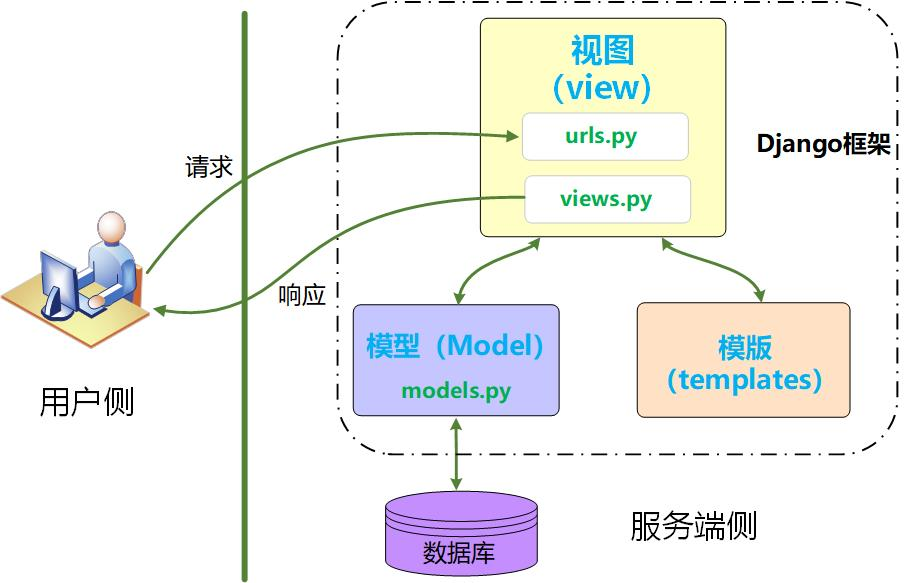
\includegraphics[width=0.75\linewidth]{django.jpg}
  \caption{Django框架示意图}
  \label{fig:django}
\end{figure}



\textbf{2)ONNX模型部署工具}

在深度学习模型训练结束后,我们要让模型能够在生产环境中运行。部署时首先要对运行环境进行配置,此外还要对网络结构进行优化精简提高模型的推理性能。
目前针对神经网络的部署主要采用深度学习框架-中间表示-推理引擎这种流水线方式。首先是定义模型结构并选择一种深度学习框架进行训练。之后,将模型结构与参数转化成一种通用的中间表示,
在此基础上进行效率优化。最后将中间表示文件在含有推理引擎的硬件平台上高效运行。

开放式神经网络交换(Open Neural Network Exchange,ONNX)是微软与Facebook在2017发布的用于描述计算图的一种格式。它是一种开放的规范,定义了模型的
标准数据类型,内置运算算子与可扩展的计算图模型。ONNX目前支持多种深度学习框架如Pytorch、Tensorflow、Caffe2、Mxnet等。在Pytorch中可以使用$torch.onnx.export()$函数将Pytorch模型
转为ONNX格式的静态计算图模型。ONNX Runtime是由微软开发的一个跨平台、高性能的机器学习推理引擎,它是ONNX文件的运行环境,在该环境下可以读取并运行.onnx 文件。
目前ONNX Runtime支持多种硬件环境,包括了CPU、GPU、地平线的BPU、华为海思等国产推理芯片。完成上述流程实现了深度学习算法的落地与部署

\textbf{3)Mysql数据库}
% 
\chapter{基于深度学习的骨髓血细胞检测算法设计与实现}
\section{引言}
骨髓血细胞形态学检查是血液疾病诊断的重要依据,主要通过人工镜检来完成,上述过程繁琐枯燥,可靠性差。
在骨髓血细胞自动化识别算法中,骨髓血细胞检测是将血细胞从涂片图像中定位并裁剪得到单一的血细胞图像,该过程是后续分类识别基础,
直接影响血液疾病诊断的结果,因此一直都是医学图像处理的热点研究方向之一。
目前基于深度学习的目标检测算法在很多领域都有广泛应用,如自动驾驶、安防监控、人脸识别、医学影像诊断等,其目的是定位或者跟踪相关目标。

根据文献调研,目前血细胞检测主要是对血细胞图像中的红细胞、白细胞与血小板进行检测。
检测算法主要基于通用的深度学习目标检测算法,包括了单阶段检测算法与两阶段检测算法。
在两阶段方法中,通过区域举荐网络生成少量感兴趣区域,并将这些区域提取到的特征输入到后续的分类与回归分支中。
在单阶段算法中,如SSD、YOLO等网络直接将全部图像作为输入,学习类别概率与边界框位置。
两类方法各有优劣,本章对这些方法进行阐述,并进行性能分析,最终选取性能较好的RetinaNet作为骨髓血细胞检测的基线模型。


\section{双阶段目标检测网络}
\label{section:faster-rcnn}
快速区域卷积网络(Faster-RCNN)是目标检测领域最为经典的双阶段检测器,其网络架构如图\ref{fig:faster_rcnn}所示,主要由
骨干网络特征提取器(BackBone)、区域举荐网络(Region proposal Network,RPN)与分类回归网络(R-CNN)这三部分组成。骨干网络为深度卷积神经网络,
用于图像特征提取。RPN网络在提取的特征图上快速生成区域坐标与相应前景分数,这些区域用于后续的分类与坐标回归。
R-CNN网络对于这些区域首先进行ROI池化(Region of Interest Pooling)将区域转换为特定大小的特征图,然后这些特征图会分别进入到
分类分支与回归分支,得到待检测目标的类别与位置信息。

\begin{figure}[htbp]  
   \centering   
   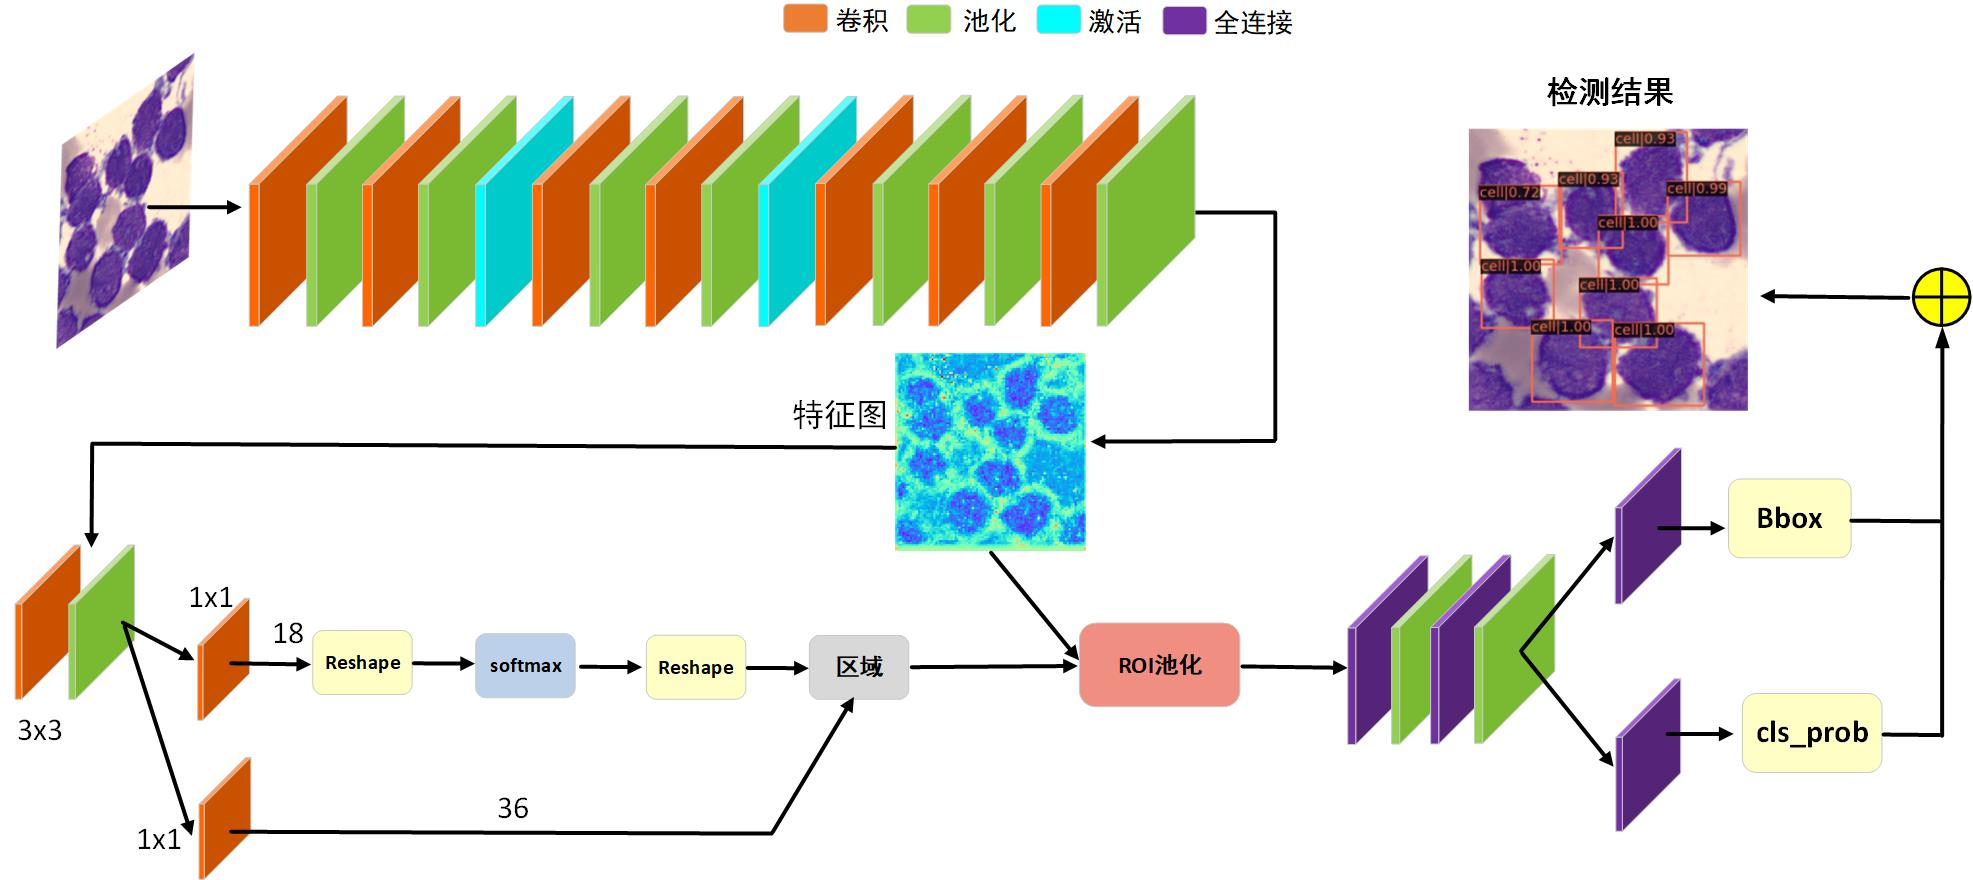
\includegraphics[width=0.9\linewidth]{faster_rcnn.jpg}   
   \caption{快速区域卷积神经网络结构示意图}   
   \label{fig:faster_rcnn} 
\end{figure}  

\subsection{骨干网络}
骨干网络是深度卷积神经网络的主体部分,用于提取图像抽象的语义特征,为后续任务提供图像的嵌入特征向量表示。
因此,骨干网络的性能对于整体网络性能具有很大的影响。常用的骨干网络有VGG、ResNet、DenseNet与Inception等,
其中ResNet是应用最为广泛的骨干网络,其特点是引入了残差模块,可以实现很深层的卷积网络。

综合考虑模型的精度、速度、参数量等因素,本节模型选择的骨干网络均为ResNet50,其结构如图~\ref{fig:resnet50}所示。
ResNet50总共由五个阶段(stage)构成,第一个阶段由一个$7\times7$的卷积组成,可视作对图像的预处理。
其余阶段均是由沙漏模块(BottleNeck)堆叠而成,第二到第五阶段分别有3、4、6、3个沙漏模块。若输入图像的大小为$224\times224\times3$
每经过一个stage,特征图的大小减小为原来的一半,通道数变为原来的两倍。五个阶段输出的特征图分别为$C_1, C_2, \dots, C_5$,
其中$C_5$特征图的大小为$7\times7\times2048$。最后特征图经过均值池化变为2048的向量,经过全连接层用于分类识别。

\begin{figure}[htbp]      
  \centering       
  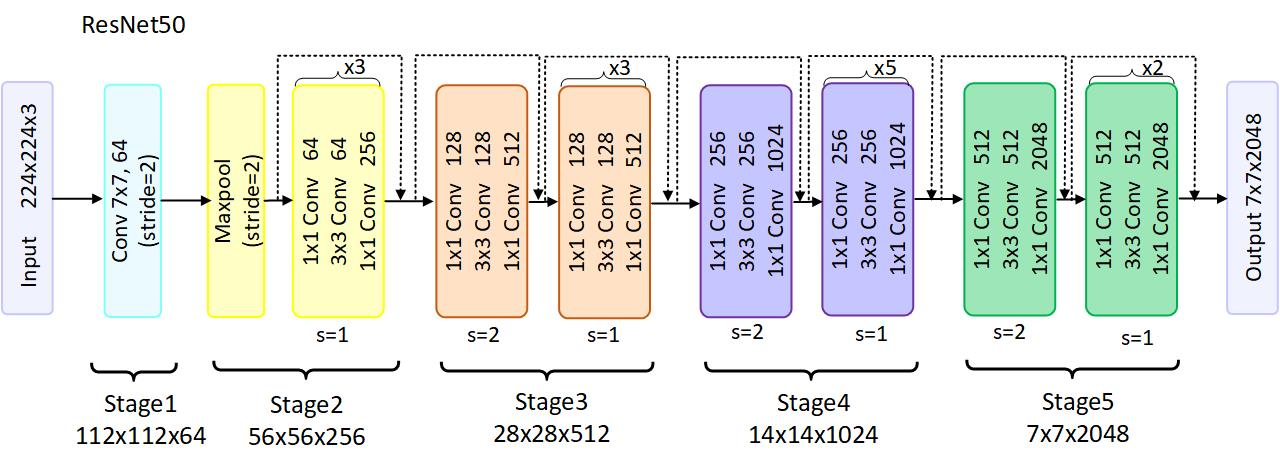
\includegraphics[width=0.9\linewidth]{resnet50.jpg}       
  \caption{ResNet50网络结构示意图}       
  \label{fig:resnet50}  
\end{figure}   

沙漏(BottleNeck)模块结构如图\ref{fig:bottleneck}所示,该网络第一个卷积层使用$1\times1$的卷积核来减少通道数量。
第二个卷积层的卷积核大小为$3\times3$,当stride为1时,特征图大小不变,stride=2时,特征图大小变为原来的一半。第三个卷积层采用$1\times1$卷积
恢复特征图的通道数。由于中间层的维度较小类似于沙漏,因此称为沙漏结构。该结构可以有效降低网络的参数量与计算量。
该结构还包括了一个残差模块,通过一个$1\times1$的卷积确保输入与输出的通道数相同后,在与输出直连相加。残差连接可以让网络更好的学习高层特征,
同时避免网络浅层部分梯度消失或爆炸等问题。图中BN为批归一化层、ReLU为激活函数。

\begin{figure}[htbp]        
  \centering          
  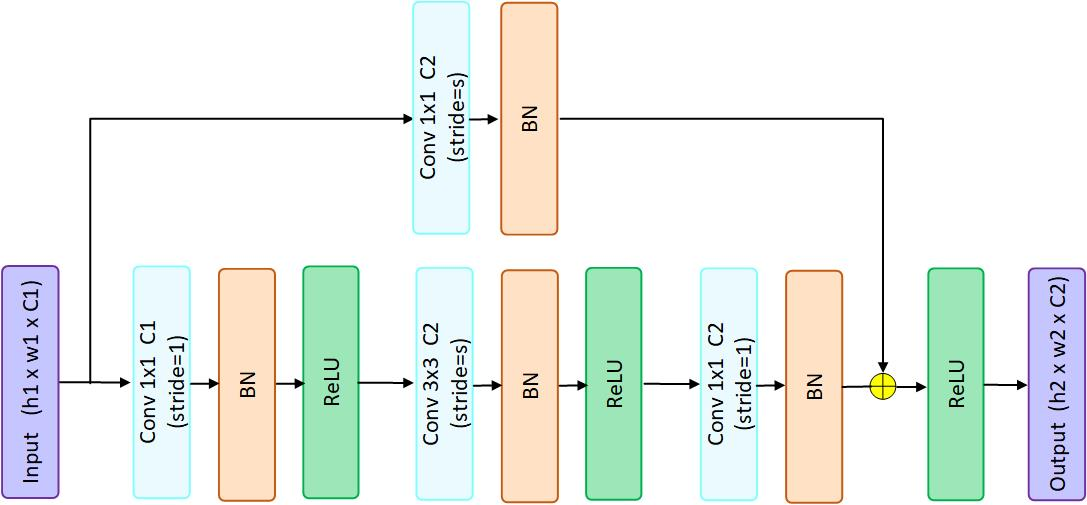
\includegraphics[width=0.7\linewidth]{bottleneck.jpg}          
  \caption{BottleNeck模块结构示意图}          
  \label{fig:bottleneck}   
\end{figure}    

\subsection{特征金字塔网络}

特征金字塔网络(Feature Pyramid Network,FPN)主要用来解决多尺度的目标检测问题。骨干网络特征提取器输出不同尺度的特征图,这些特征图的感受野不同。
高层特征图感受野比较大,用来检测大尺寸目标,浅层的特征图感受野较小,用来检测小尺寸目标。
但是浅层特征图的表达能力较弱,通常只有纹理、边缘形状、明暗等细节信息,而高层特征图则包含更加丰富的全局信息。
为解决浅层网络特征表达能力有限的问题,Lin等\cite{2017Feature}引入了特征金字塔网络。该网络将顶层特征逐级向下传递并与浅层特征融合,
使得浅层特征可以同时兼顾细节与整体具有更加丰富的特征表达。ResNet50骨干网络构建特征金字塔的结构如图~\ref{fig:fpn}所示。
图中$C_1,C_2 \cdots C_5$为ResNet骨干网络生成的不同尺度特征图,相邻两个阶段的特征图在尺寸上为二倍缩放的关系。
自顶向下的融合过程经过上采样与通道调整使得特征图的尺寸一致后再相加融合。以$P_4$特征图的生成为例,$P_5$由$C_5$特征图经过$1\times1$、通道数为256的卷积层得到。
$P_5$经过二倍上采样(由反卷积实现)与$C_4$经过$1\times1$、通道数为256的卷积的结果相加得到$P_4$。其他特征图同样由上述过程生成。
最后FPN使用$3 \times 3$卷积对融合后的特征图进行平滑处理消除直接相加可能导致的融合不充分问题。至此,完成了特征金字塔的构建。

\begin{figure}[htbp]            
  \centering             
  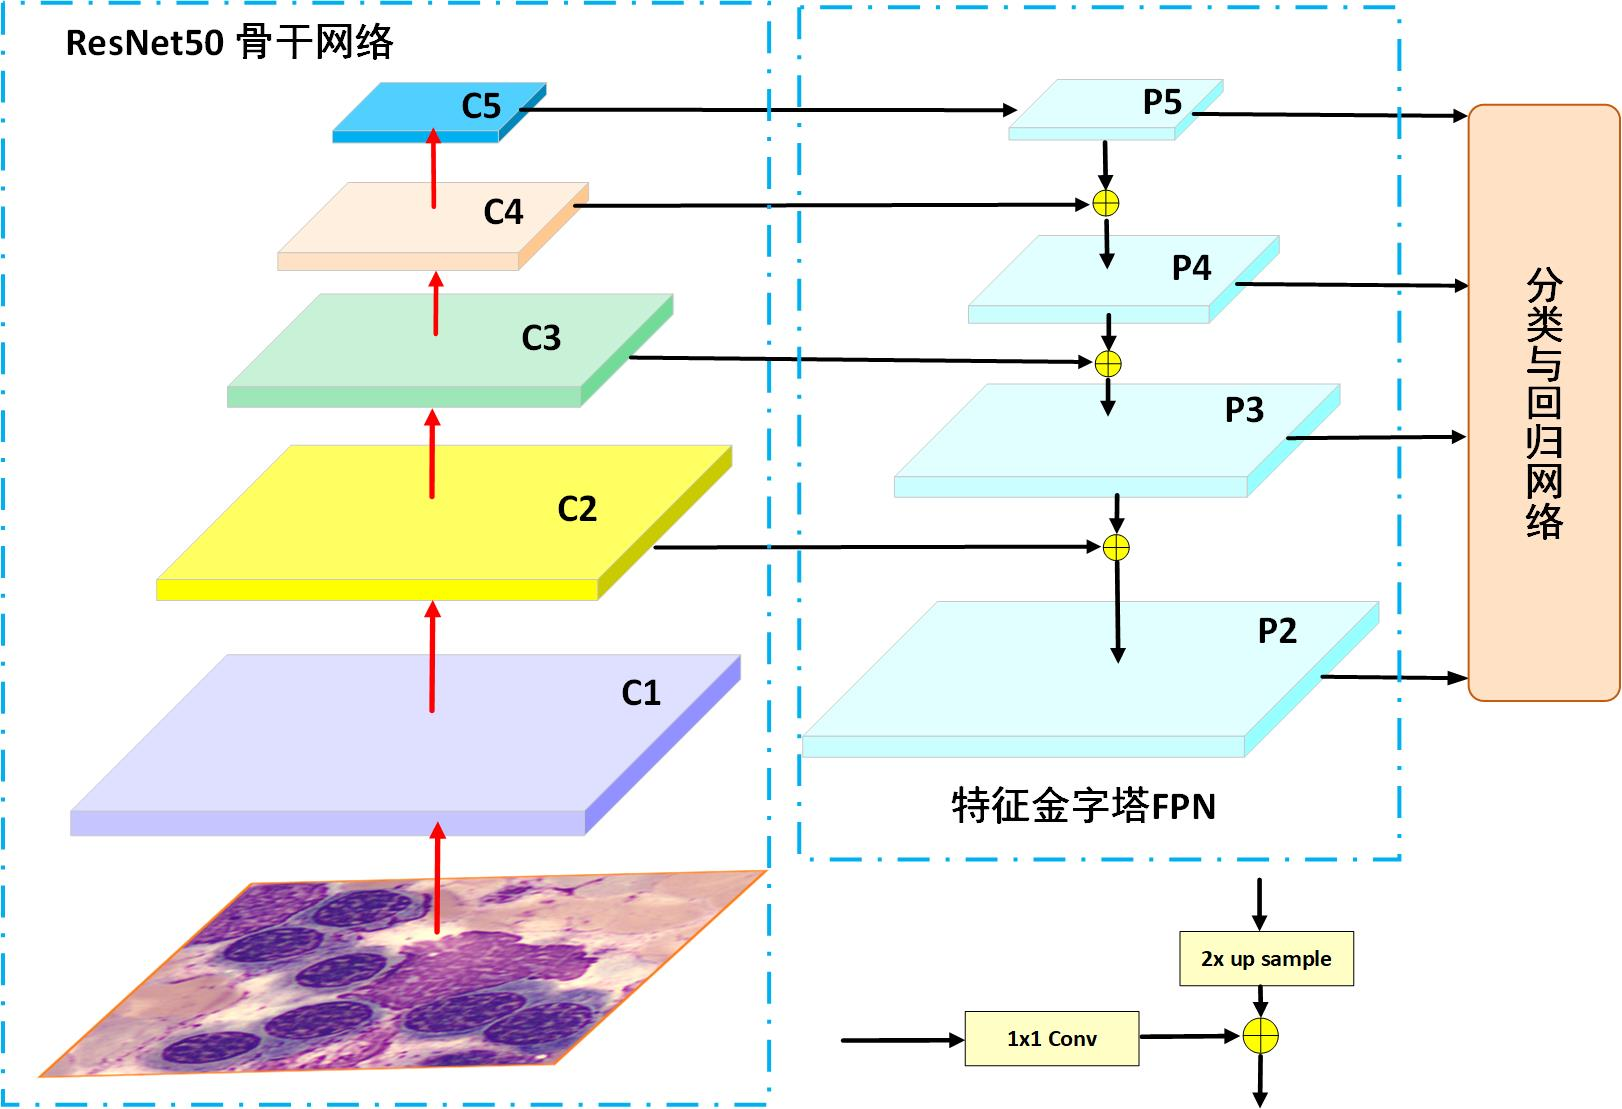
\includegraphics[width=0.65\linewidth]{fpn.jpg}             
  \caption{特征金字塔网络结构示意图}             
  \label{fig:fpn}    
\end{figure}    

\subsection{区域举荐网络}

区举荐网络(Region Proposal Network, RPN)基于骨干网络提取的特征图生成一系列候选框区域,用于后续分类识别。
RPN网络结构如图~\ref{fig:rpn}所示,包含了两个分支,上面一条分支用于预测每个锚框属于前景的分数。
下面一条分支用于计算锚框边界坐标的回归信息,以生成更加精准的区域坐标。最后生成的候选框区域综合了前景分数与坐标修正,
实现了目标的初步定位。

\begin{figure}[htbp]              
  \centering                
  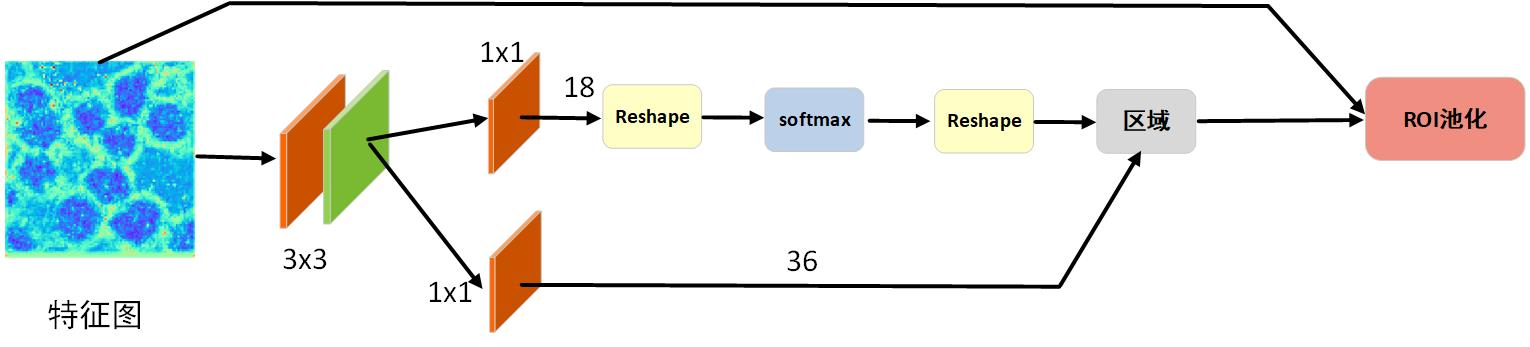
\includegraphics[width=0.90\linewidth]{rpn.jpg}                
  \caption{特征金字塔网络结构示意图}                
  \label{fig:rpn}     
\end{figure}   

锚框是RPN网络根据预先定义的参数生成的一些列矩形区域,对于特征图上的每个锚点会生成$k$个锚框,通常将$k$设置为$9$。如图\ref{fig:anchor}(a)所示,
九个锚框有三种尺寸与三种长宽比,锚框尺寸由数据集目标先验信息与特征图大小决定,
尺度变化范围为$2^0, 2^{\frac{1}{3}},  2^{\frac{2}{3}}$,长宽比通常设定为$0.5, 1, 2$。以骨髓血细胞图像为例,原图尺寸为
$363 \times 360 \times 3$,首先经过缩放与填充转大小换为$832 \times 800 \times 3$,所有anchor的尺寸在$32 \times 32$ \textasciitilde
$812 \times 812$,几乎可以覆盖各个尺寸的目标。以$P_2$特征图为例,该特征图的尺寸为$208 \times 200$,缩放尺度为4,九种anchor的尺寸分别为
$23 \times 45,\quad32 \times 32,\quad45 \times 23,\quad29 \times 57,\quad40 \times 40,\quad57 \times 29,\quad36 \times 72,\quad51 \times 51,\quad72 \times 36$。

\begin{figure}[htbp]
	\centering
	\begin{subfigure}{0.45\linewidth}
		\centering
		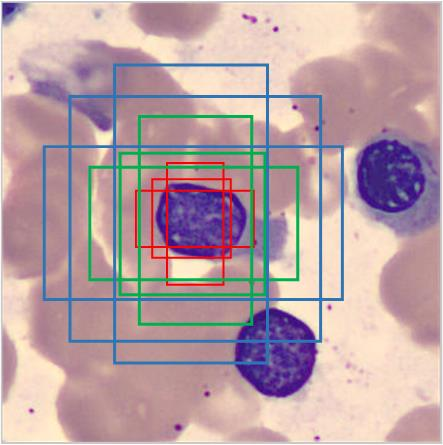
\includegraphics[width=0.95\linewidth, height=0.95\linewidth]{anchor_a.jpg}
    \caption{}
	\end{subfigure}
	\centering
	\begin{subfigure}{0.45\linewidth}
		\centering
		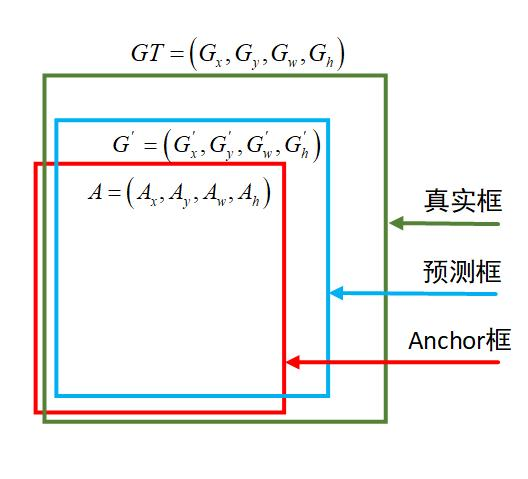
\includegraphics[width=0.95\linewidth, height=0.95\linewidth]{anchor_b.jpg}
    \caption{}
	\end{subfigure}
	\caption{(a) Anchor在图像中的示意图, (b) Anchor、预测框与真值框之间的关系}
	\label{fig:anchor}
\end{figure}

特征图经过预测前景分支后输出的尺寸为$h\times w \times 2k$,
对应锚点的$k$个锚框,每个锚框有前景与背景两种分数。经过坐标回归分支后得到尺寸为$h\times w \times 4k$的
坐标回归结果。我们采用$(x, y, w, h)$这样的四维向量来表示矩形框,分别代表矩形框的中心与宽高。
如图\ref{fig:anchor}(b)所示, 红色框A为按照预先定义生成的锚框$A = \left( {{A_x},{A_y},{A_w},{A_h}} \right)$,
绿色框代表目标的真值框$GT = \left( {{G_x},{G_y},{G_w},{G_h}} \right)$。坐标回归分支希望学习到一个映射
$F\left(A_{x}, A_{y}, A_{w}, A_{h}\right)=\left(G_{x}^{\prime}, G_{y}^{\prime}, G_{w}^{\prime}, G_{h}^{\prime}\right)$,
使得原始的锚框A经过映射后得到的预测框$G^{\prime}$能够更加接近真实框$GT$。

变换$F$中包含的参数通过坐标回归分支得到$d_{*}(A)=W_{*}^{T} \cdot \phi(A)$,其中$\phi(A)$为锚点对应的特征向量,
$W_{*}$为$1\times1$卷积层需学习的参数,$d_{*}(A)=d_{x}(A), d_{y}(A), d_{w}(A), d_{h}(A)$,锚框A与预测框$G^{\prime}$
的坐标关系如式~\ref{eq:bbox_reg1}所示。
\begin{equation}
  \begin{array}{cc}
    G_{x}^{\prime} =A_{w} \cdot d_{x}(A)+A_{x} & G_{y}^{\prime} = A_{h} \cdot d_{y}(A)+A_{y} \\
    G_{w}^{\prime} =A_{w} \cdot \exp \left(d_{w}(A)\right) & G_{h}^{\prime} =A_{h} \cdot \exp \left(d_{h}(A)\right)
  \end{array}
  \label{eq:bbox_reg1}
\end{equation}

真实框GT与锚框A之间的平移量$(t_{x}, t_{y})$与尺度因子$(t_{w}, t_{h})$的变换计算如式~\ref{eq:bbox_reg2}所示。
\begin{equation}
  \begin{array}{cc}
    t_{x}=\left(G_{x}-+A_{x}\right) / A_{w} & t_{y}=\left(G_{y}-A_{y}\right) / A_{h} \\
    t_{w}=\log \left(G_{w} / A_{w}\right) & t_{h}=\log \left(G_{h} / A_{h}\right)
  \end{array}
  \label{eq:bbox_reg2}
\end{equation}

坐标回归分支网络在训练时的优化目标是让预测值$d_{*}(A)$与真实变换系数$t_{*}$之间的差距最小,选择smooth-L1损失函数进行优化。
在测试时,网络输出修正的坐标变换信息将锚框修正,用于后续处理。
\begin{equation}
  {\hat W_*} = {{\mathop{\rm argmin}\nolimits} _{{W_*}}}\sum\limits_i^n {{{{\mathop{\rm smooth}\nolimits} }_{{L_1}}}
  \left( {t_*^i - W_*^T \cdot \phi ({A^i})} \right)}  + \lambda \left\| {{W_*}} \right\|
  \label{eq:bbox_reg3}
\end{equation}
\begin{equation}
  \operatorname{smooth}_{L_{1}}(x)
  =\left\{\begin{array}{rr} 0.5 x^{2} & \text { if }|x|<1 \\ |x|-0.5 & \text { otherswise, } \end{array}\right.
  \label{eq:bbox_reg4}
\end{equation}

\subsection{分类与回归网络}
RPN网络生成的候选区域大小形状各不相同,需要经过ROI池化保证尺寸相同。首先将候选区域对应位置映射到特征图上,将对应特征图区域
划分为$pool_w \times pool_h$的网格,在每个网格区域内进行最大池化,这样每个区域转化为$pool_w \times pool_h$固定大小输出。

\begin{figure}[htbp]                  
  \centering                   
  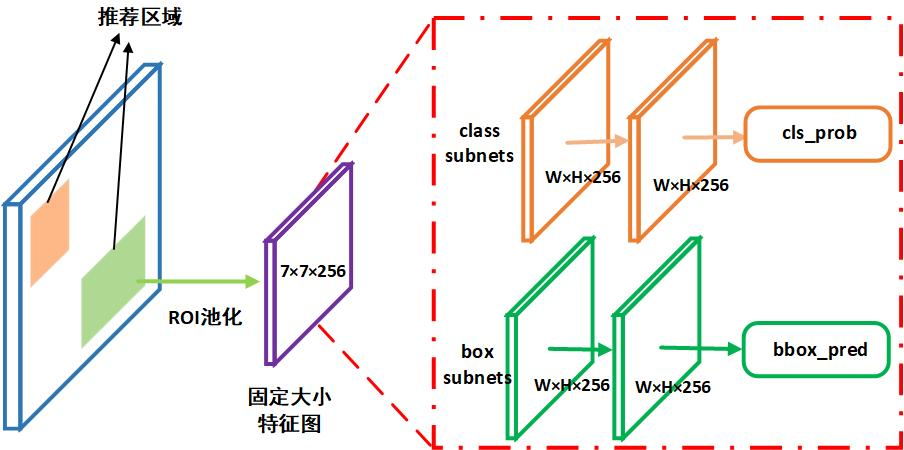
\includegraphics[width=0.75\linewidth]{subnets.jpg}                   
  \caption{分类与回归网络结构示意图}                   
  \label{fig:subnets}      
\end{figure}   

分类网络使用ROI池化后的特征图,经过全连接层与Softmax函数输出分类概率向量,在训练时使用交叉熵损失函数进行优化。
回归分支与RPN网络部分的坐标回归分支类似,目的是为了获得更加精确的检测框坐标。

\section{单阶段目标检测网络}

\subsection{网络结构}
单阶段检测器如SSD、RetianNet、YOLO系列等具有较快的检测速度与较高的检测精度,通常用于实时目标检测。
单阶段检测器在特征图上进行密集检测,对所有的锚框均进行分类与回归。
在图像中大量的锚框都属于负样本,因此单阶段检测器在训练阶段面临着严重的正负样本不均衡问题,大量易分的负样本
主导了损失函数的训练,使得网络难以对正样本进行学习,影响参数收敛,网络性能差。
两阶段网络如Faster-RCNN通过区域举荐网络对所有锚框进行前景分数预测,并将可能包含目标的少量候选框传给后续的分类回归网络进行识别,
有效的控制了正负样本比例,很好的解决了上述问题。

为解决单阶段检测器中极度不平衡的正负样本问题,Lin~\cite{lin2017focal}等提出了一种简单且实用的焦点损失函数(Focal Loss),并设计了RetianNet网络。
在该损失函数引导下,网络增加了对难以区分正样本的关注,减少了对易分辨背景样本的关注。RetinaNet网络结构如图~\ref{fig:retinanet}所示,由骨干网络、特征金字塔网络与分类回归网络组成,
网络主体结构在~\ref{section:faster-rcnn}节已进行详细阐述。

\begin{figure}[htbp]                     
  \centering                      
  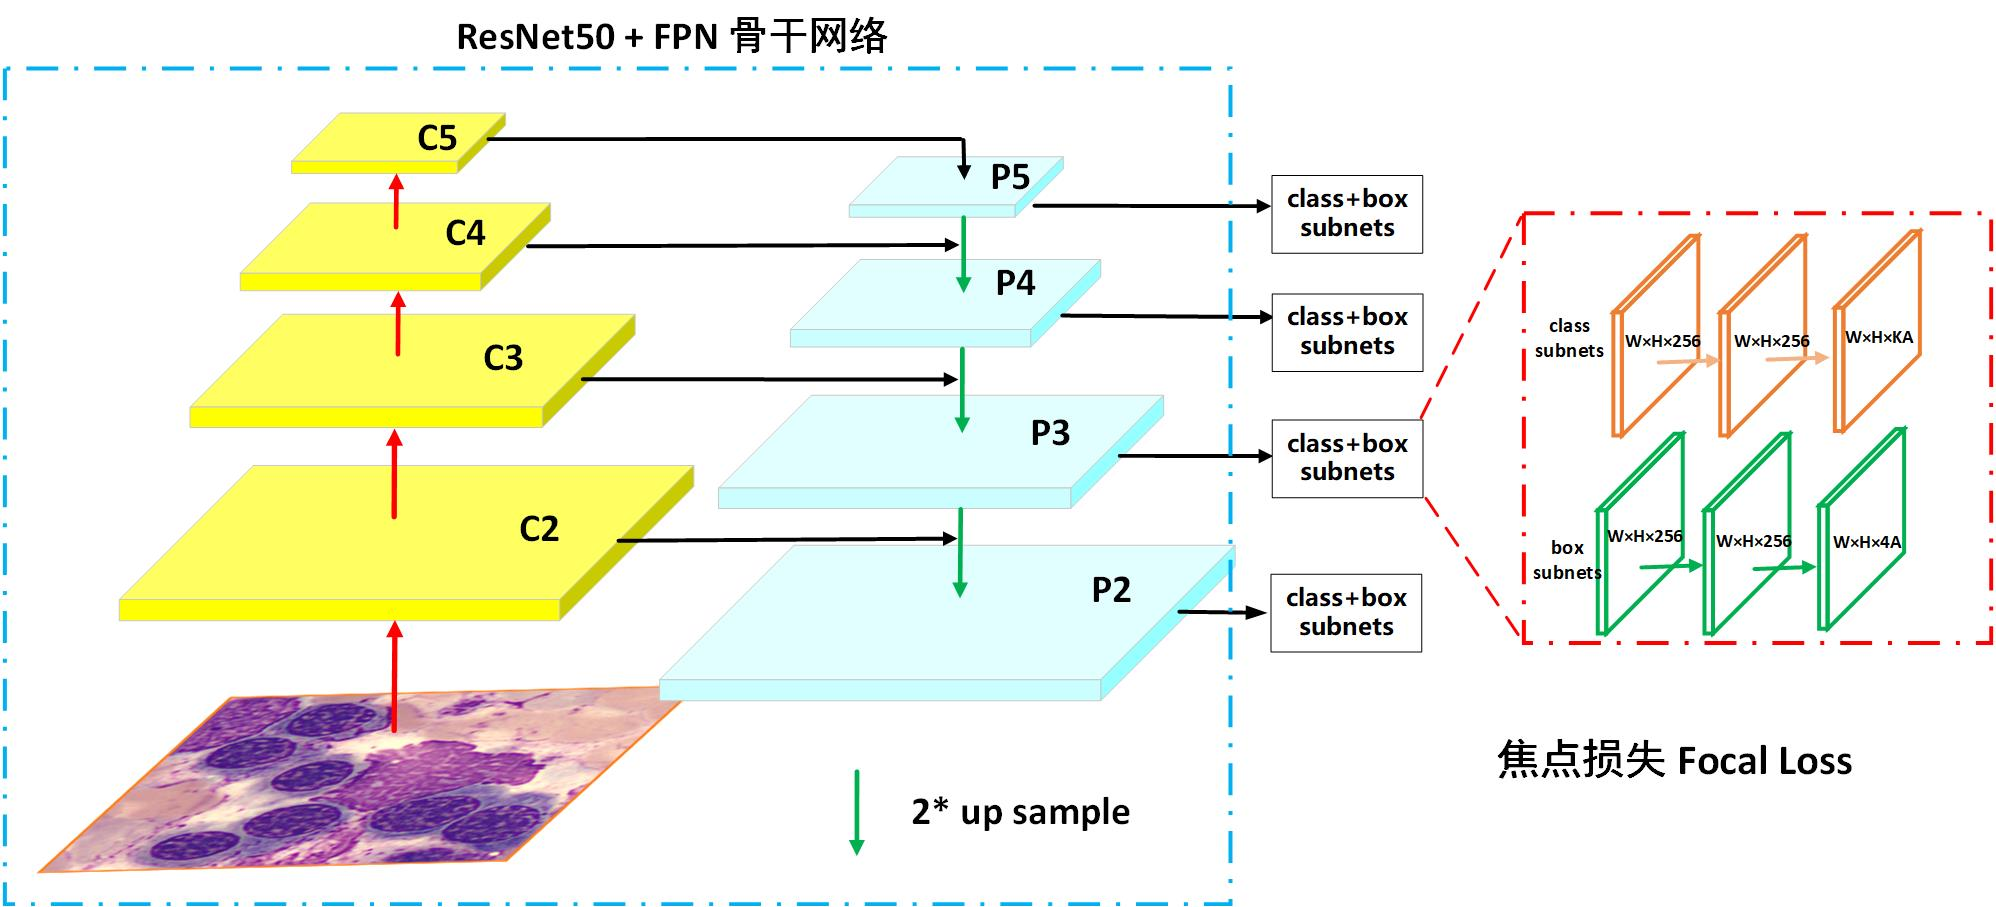
\includegraphics[width=0.80\linewidth]{retinanet.jpg}                      
  \caption{分类与回归网络结构示意图}                      
  \label{fig:retinanet}       
\end{figure}   

\subsection{焦点损失函数}
焦点损失是基于交叉损失函数提出,在深度学习中,交叉熵用来衡量模型预测结果分布与真实结果分布之间的差异性,一般用于分类任务。
假设有$N$个样本,类别数为$C$,$y_{ij}$表示第$i$个样本属于第$j$类的标签,取值为$0, 1$。$\hat{y_{ij}}$表示模型预测第$i$个样本属于第$j$
的概率,则交叉熵损失函数如式~\ref{eq:ce_loss}所示:
\begin{equation}   
  {\rm{CE}}\_{\rm{Loss}}(y,\hat y) =  - \frac{1}{N}\sum\limits_{i = 1}^N {\sum\limits_{j = 1}^C {{y_{ij}}} } \log \left( {\widehat {{y_{ij}}}} \right)
  \label{eq:ce_loss} 
\end{equation}

在二分类问题中,只有两个正负样本,若$p$表示预测为正样本的概率,$1-p$表示预测为负样本的概率,样本标签取值为$0,1$,则二元交叉熵如式所~\ref{eq:bce_loss}示:
\begin{equation}         
  \operatorname{BCE}=\left\{\begin{array}{ccc} -\log (p), & \text { if } & y=1 \\ -\log (1-p), & \text { if } & y=0 \end{array}\right.  
  \label{eq:bce_loss}   
\end{equation} 

常见解决正负样本不平衡的方法是引入$\alpha$参数平衡正负样本损失函数的权重。该参数由正负样本比例决定$\frac{\alpha}{1-\alpha} = \frac{n}{m}$,式中$n$为负样本数量,
$m$为正样本数量。
\begin{equation}            
  \operatorname{BCE}=\left\{\begin{array}{ccc} -\alpha \log (p), & \text { if } & y=1 \\ -(1-\alpha) \log (1-p), & \text { if } & y=0 \end{array}\right.    
  \label{eq:bce_loss_alpha}    
\end{equation} 

焦点损失在平衡二元交叉熵损失基础上加入了难易调整因子$\gamma$,训练过程中,大量的锚框都属于易分的背景样本,这些置信度较高的样本
对于模型效果提升影响较小。焦点损失对于高置信度样本进行惩罚,降低其损失函数中的权重$(1-p_t)^{\gamma}$,使得网络关注到难分的正负样本。
焦点损失如式~\ref{eq:focal_loss}所示。$\gamma=0$时焦点损失等价于平衡二元交叉熵损失函数,$\gamma=2$时网络的效果较好,当分类概率$p_t$为0.9时,其损失函数权重降低100倍。
而分类概率$p_t = 0.5$时,损失函数权重仅降低四倍。这使得网络在训练时能不断地聚焦在那些学习较差的样本上,梯度更新方法主要困难样本决定。$\alpha$是类别权重,正负样本的$\alpha$通常设置为
$(0.25, 0.75)$。
\begin{equation}               
  \begin{array}{*{20}{c}} {{\rm{Focal\_Loss}}\left( {{p_t}} \right) =  - \alpha {{\left( {1 - {p_t}} \right)}^\gamma }\log \left( {{p_t}} \right)}\\ 
    {{p_t} = \left\{ {\begin{array}{*{20}{c}} {p,}&{{\rm{ if }}}&{y = 1}\\ {1 - p,}&{{\rm{ if }}}&{y = 0} \end{array}} \right.} \end{array}    
  \label{eq:focal_loss}     
\end{equation} 

\subsection{网络预测}

在网络的预测推理阶段,RetinaNet在特征金字塔输出的多尺度特征图上进行预测。对于骨髓血细胞图像首先通过双线性插值缩放到$832 \times 800$大小,
其特征图$P_2, P_3 \cdots, P_5$的大小分别为$208 \times 200$、$104 \times 100$、$52 \times 50$、$ 26 \times 25$、$13 * 13$,特征图上的每个锚点
输出9个锚框,对于一张骨髓血细胞图像,网络总共输出$55250 \times 9$个检测结果。每个检测结果包括了一个分类置信度向量与一个四维坐标回归向量,
根据坐标回归向量可以计算出检测框在原始图像上的坐标。对于每个骨髓血细胞类别,大量的检测框均为背景区域,首先将置信度低于0.05的检测框滤除。
然后对检测框按照置信度从高到低进行排序,选取前1000个检测框进行非极大值抑制(Non-Maximum Suppresion,NMS)去除重复的检测框。NMS的过程如下:
首先从置信度最高的框开始,计算它与剩余框的交并比(IOU),并去除交并比大于阈值(通常为0.5)的框。然后在剩余框中继续选择置信度最高的框重复上述过程,
最后保留的框为非极大值抑制后处理后的结果。最终合并所有血细胞类别的检测结果,选择置信度最大的前100个框作为当前图片的检测框结果。


\section{算法实现与实验结果分析}

研究初期,我们需要对比不同目标检测网络的性能,确定骨髓血细胞检测的基线模型,然后在此基础上进行改进。
在双阶段网络中,我们选择了Faster-RCNN、Cascade-RCNN网络,在单阶段网络中,我们选择RetinaNet与YOLOV3。
上述网络都是经典的具有代表性的检测网络。我们比较了不同网络的参数量与浮点计算量与在骨髓血细胞数据集上的检测精度。
此外,我们探索了网络在仅做检测与检测识别一体化任务上性能的差异。

\subsection{实验环境}

\subsubsection{数据集介绍}

骨髓血细胞图像来自邃蓝智能科技(上海)有限公司合作医院提供,首先采用第2.1小节阐述的主动学习标注策略进行边界框的标注。
我们总共标记了6821张血细胞图像,训练集与测试集按照4:1的比例进行随机划分,训练集包含了5456张图像,测试集包含了1365张图像。
通常每个图像中包含1到10个有核血细胞,数据集总共标记了11352个血细胞,训练集有9065个血细胞,测试集有2287个血细胞。数据集的分布如
表~\ref{table:cell_detect}所示:

\begin{table}
  \caption{骨髓血细胞检测数据集分布}   
  \centering 
  \label{table:cell_detect}
  \begin{tabular}{ccccc}
    \toprule[2pt]
    序号 & 类别名  &  类别简写 & 训练集数量 & 测试集数量 \\
    \midrule[1.5pt] 
    1 & 原始细胞 & Prim & 1856 & 467 \\ 
    2 & 淋巴细胞 & Lym & 996 & 226   \\ 
    3 & 单核细胞 & Mono & 206 & 52   \\ 
    4 & 浆细胞 & Plas & 272 & 70   \\ 
    5 & 红细胞 & Red & 1880 & 503   \\ 
    6 & 早幼粒细胞 & Promy & 357 & 107   \\ 
    7 & 嗜中性中幼粒细胞 & Myelo & 701 & 150   \\ 
    8 & 嗜中性晚幼粒细胞 & Late & 503 & 144   \\ 
    9 & 嗜中性杆状核细胞 & Rods & 998 & 241   \\  
    10 & 嗜中分叶核细胞 & Lobu & 821 & 195   \\  
    11 & 嗜酸性粒细胞 & Eosl & 475 & 132   \\  
    \hline
    总计 &   &   & 9065 & 2287 \\
    \bottomrule[2pt]      
  \end{tabular} 
\end{table}

\subsubsection{评价指标}

在目标检测领域,通常使用检测框与真实框的交并比(IOU)来判断检测框是属于正样本还是负样本。交并比的定义如图~\ref{fig:iou}所示,对于预测框A与真实框B,
IOU值等于两个矩形框的交集面积$S(A \cap B)$与并集面积$S(A \cup B)$的比值。IOU的取值范围为$0 \sim 1$,值越大表示两个矩形相似程度越高。
\begin{figure}[htbp]                     
  \centering                      
  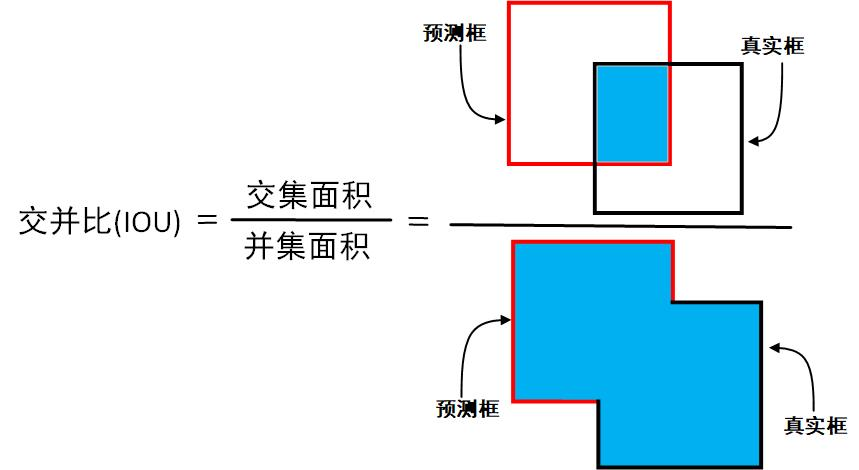
\includegraphics[width=0.60\linewidth]{iou.jpg}                      
  \caption{IOU计算示意图}                      
  \label{fig:iou}       
\end{figure}   

在深度学习中,TP(True Positive)表示被正确检测为正类的正样本;FP(False Positive)表示被错误检测为正类的负样本;
TN(True Negative)表示被正确检测为负类的负样本。FN(False Negative)表示被错误检测为负类的正样本。
对于检测任务,需要根据检测框的置信度分数与交并比来判断
以图~\ref{fig:confusion}为例,绿色框为真实框,红色框为网络检出框。
第一张图中检测框与真实框IOU大于阈值,且类别正确,为真正例TP。第二张图中IOU大于阈值,但是类别检测错误,分叶核(Lobu)真实类别被错误检测为杆状核(Rods)类别(FP)。
第三张图中,检测框与所有真实框IOU均小于阈值,背景类被错误检测为Lobu类(FP)。第四张图片未检出,Lobu类别被错误检测为背景类(FN)。

\begin{figure}[htbp]
	\centering
  \begin{subfigure}{0.24\linewidth}
    \centering
    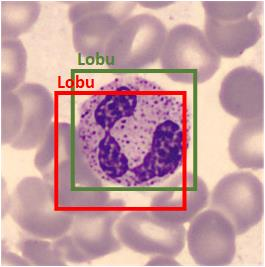
\includegraphics[width=0.95\linewidth, height=0.95\linewidth]{det1.jpg}
    \caption{检测正确TP}
  \end{subfigure}
	\centering
	\begin{subfigure}{0.24\linewidth}
		\centering
		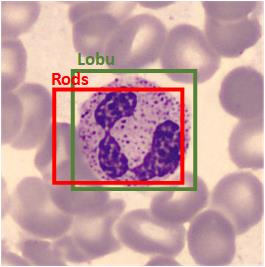
\includegraphics[width=0.95\linewidth, height=0.95\linewidth]{det2.jpg}
    \caption{分类错误FP}
	\end{subfigure}
	\centering
	\begin{subfigure}{0.24\linewidth}
		\centering
		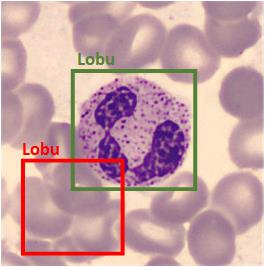
\includegraphics[width=0.95\linewidth, height=0.95\linewidth]{det3.jpg}
    \caption{IOU小于阈值BG}
	\end{subfigure}
	\centering
	\begin{subfigure}{0.24\linewidth}
		\centering
		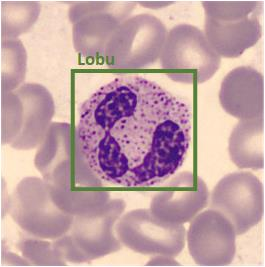
\includegraphics[width=0.95\linewidth, height=0.95\linewidth]{det4.jpg}
    \caption{未检出FN}
	\end{subfigure}
	\caption{检测类型判别}
	\label{fig:confusion}
\end{figure}

目标检测常用的评价指标有精准率(precision)、召回率(recall)、PR曲线、平均精度(Average Precision,AP)与平均精度均值(Mean Average Precision,mAP)。

精准率是指预测正确的正样本数量与所有预测为正样本数量的比值,如式~\ref{eq:precision}所示:
\begin{equation}               
  Precision = \frac{TP}{TP + FP}
  \label{eq:precision}     
\end{equation} 

召回率是指预测正确正样本数量与所有正样本数量的比值,如式~\ref{eq:recall}所示
\begin{equation}               
  Precision = \frac{TP}{TP + FN}
  \label{eq:recall}     
\end{equation} 

PR曲线是以召回率为横坐标,以精确率为纵坐标绘制的曲线。在绘制某一类别PR曲线时,将检测框按照置信度从高到低
进行排序,设定多组置信度阈值,根据交并比会得到多组精确率与召回率,最后将这些点连接起来得到最终的PR曲线。
随着召回率的提高,检测的精确率会降低,曲线越靠近右上角代表网络的检测性能越好
平均精度是PR曲线下的面积,即在多组召回率下的平均检测精确率。AP值越大代表模型的性能越好。
平均精度均值(mAP)是对所有类别的平均精度求均值,通常用来衡量网络的检测效果。

\subsubsection{实验设置}
我们在Linux操作系统下的NVIDIA TITAN V显卡上训练模型。训练使用的深度学习框架为Pytorch1.13.1,批量大小设置为16。
优化器使用随机梯度下降算法(SGD),动量设置为0.9,权重衰减设置为5e-4。学习率初始化为0.001,网络总共训练36个轮次,
在第16与第28个轮次,学习率变为原来的$1/10$。RetianNet中Focal Loss中正负样本平衡参数$\alpha=0.25$,难易调整参数$\gamma=2$。
数据集原始图像大小为$363 \times 300$,为了更好的检测小目标,图像经过双线性插值与填充扩大到$832 \times 800$。
我们基于迁移学习的方式进行训练,单双阶段网络参数初始化均使用在COCO数据集上预训练的模型,然后使用骨髓学习检测数据集进行微调。

\subsection{实验结果与分析}
\subsubsection{参数量、计算量与速度}

Faster-RCNN、Cascade-RCNN、RetinaNet与YOLOV3四种网络在输入图像大小为$832 \times 800$的情况下的参数量与计算量
如表~\ref{table:cell_Network}所示。我们比较了四种网络在NVIDIA TITAN V硬件环境下的每秒帧率(Frame Per Second,FPS),即每秒可以处理的
图像数量,来评估网络是否可以满足在生产环境实时性的要求。

\begin{table}
  \caption{不同网络结构参数量、计算量与速度对比}   
  \centering 
  \label{table:cell_Network}
  \begin{tabular}{ccccc}
    \toprule[2pt]
    方法 & 骨干网络  & 参数量(MB) & 计算量(GFLOPs) & FPS (TITAN V) \\
    \midrule[1.5pt] 
    Faster-RCNN & ResNet50 &  41.17 & 139.25 & 27.7 \\ 
    Cascade-RCNN & ResNet50 & 69.17 & 167.24 & 21.9   \\ 
    RetinaNet & ResNet50 & 36.31 & 135.73 & 29.5   \\ 
    YOLOV3 & DarkNet53 & 61.95 & 127.11 & 32.3  \\ 
    \bottomrule[2pt]      
  \end{tabular} 
\end{table}

从表中可以看出,四种网络的FPS均大于20,可以满足骨髓血细胞检测速度实时性的要求。
单阶段网络的速度高于双阶段的目标检测网络。RetinaNet网络参数量最小,计算消耗资源也相对较少,更适合在生产环境中进行部署。


\subsubsection{检测算法精度对比}

四种检测网络在骨髓血细胞测试集上的结果如表~\ref{table:cell_test}所示,其中$\text{AP}_{Prim}$表示原始细胞在$IOU=0.75$下的$\text{AP}$值,
其他$\text{AP}_{*}$代表各类血细胞的$\text{AP}$值。$\text{mAP}$为所有类别$\text{AP}$的平均值,可以直观的衡量网络检测效果。

\begin{table}   
  \caption{不同目标检测方法在骨髓血细胞测试集上的检测结果}      
  \centering    
  \label{table:cell_test}
  \resizebox{0.95\linewidth}{!}{ 
  \begin{tabular}{ccccccc}     
    \toprule[1pt]     
    方法 & $\text{AP}_{prim}$ & $\text{AP}_{lym}$ & $\text{AP}_{mono}$ &  $\text{AP}_{plas}$ & $\text{AP}_{red}$ & $\text{AP}_{promy}$    \\ 
    \midrule[1pt]      
    Faster-RCNN  & 0.861 & 0.690 & 0.262 & 0.715 & 0.871 & 0.640  \\      
    Cascade-RCNN & 0.860 & 0.621 & 0.409 & 0.683 & 0.875 & 0.620  \\      
    RetinaNet    & $\pmb{0.879}$ & 0.713 & 0.402 & $\pmb{0.721}$ & $\pmb{0.928}$ & 0.662  \\      
    YOLOV3       & 0.840 & 0.784 & 0.385 & 0.705 & 0.908 & 0.540 \\      
    \bottomrule[1pt]         
  \end{tabular} 
  }
  \centering  
  \resizebox{0.95\linewidth}{!}{ 
  \begin{tabular}{ccccccc}                 
    方法 & $\text{AP}_{myelo}$  &$\text{AP}_{late}$ & $\text{AP}_{rods}$ & $\text{AP}_{lobu}$ &  $\text{AP}_{eosl}$ & $\text{mAP}$ \\          
    \midrule[1pt]           
    Faster-RCNN  & 0.678 & 0.656 & 0.672 & 0.712 & 0.754 & 0.682 \\     
    Cascade-RCNN & 0.721 & 0.724 & 0.787 & 0.846 & 0.775 & $\pmb{0.719}$   \\          
    RetinaNet    & $\pmb{0.750}$ & 0.558 & 0.638 & 0.847 & 0.735 &  0.709   \\      
    YOLOV3       & 0.714 & 0.664 & 0.769 & 0.793 & 0.766 &  0.699 \\       
    \bottomrule[1pt]            
  \end{tabular} 
  }  
\end{table} 

从表中可以看出,所有检测器针对单核细胞(Mono)的检测效果较差。$\text{AP}$值均小于$0.5$,
针对有核红细胞的检测效果最好,$\text{AP}$值大于$0.85$,单核细胞在数据集中样本数量最少,有核红细胞在数据集中的
样本数量最多,因此网络学习的效果与数据集中的样本量有关,需要增加类别较差样本的数量来提升该类血细胞的检测精度。
平均检测精度(mAP)最高的网络为双阶段网络Cascade-RCNN,单阶网络RetinaNet次之,Faster-RCNN检测精度最差。RetinaNet在多类血细胞如原始细胞、浆细胞、
红细胞等平均检测精度最高,虽然平均检测精度稍低于Cascade-RCNN,但相比于Cascade-RCNN的计算量更少与速度更快,具有更高的性价比。

\begin{figure}[htbp]                     
  \centering                      
  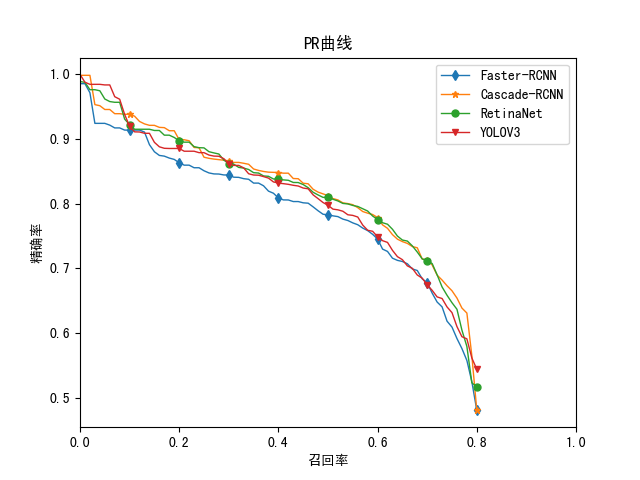
\includegraphics[width=0.6\linewidth]{PR_net.png}                      
  \caption{四种检测网络的PR曲线(IOU=0.75)}                      
  \label{fig:pr_net}       
\end{figure}   

骨髓血细胞检测是多类别检测问题,对于每一类血细胞都有自己的精确率与召回率关系。为了更加直观的比较不同网络的结果,
对于某一召回率,我们计算所有类别的平均精确率来绘制PR曲线。四种网络在$\text{IOU}=0.75$的条件下PR曲线如图~\ref{fig:pr_net}所示。
四种网络每类血细胞的PR曲线如图~\ref{fig:pr_curve}(a)-(d)所示。

\begin{figure}[htbp]
	\centering
  \begin{subfigure}{0.48\linewidth}
    \centering
    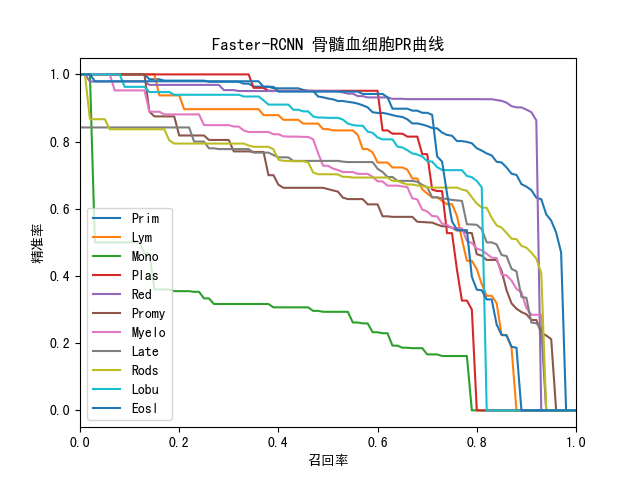
\includegraphics[width=1.0\linewidth, height=0.75\linewidth]{PR_1.png}
    \caption{Faster-RCNN网络PR曲线}
  \end{subfigure}
  \begin{subfigure}{0.48\linewidth}
    \centering
    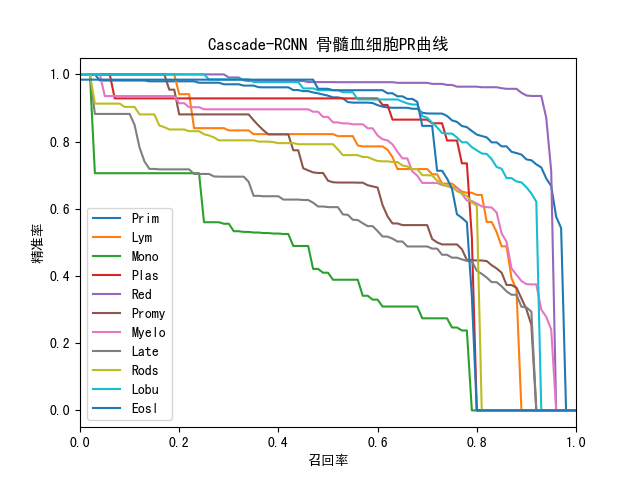
\includegraphics[width=1.0\linewidth, height=0.75\linewidth]{PR_2.png}
    \caption{Cascade-RCNN网络PR曲线}
  \end{subfigure}
	\centering
  \begin{subfigure}{0.48\linewidth}
    \centering
    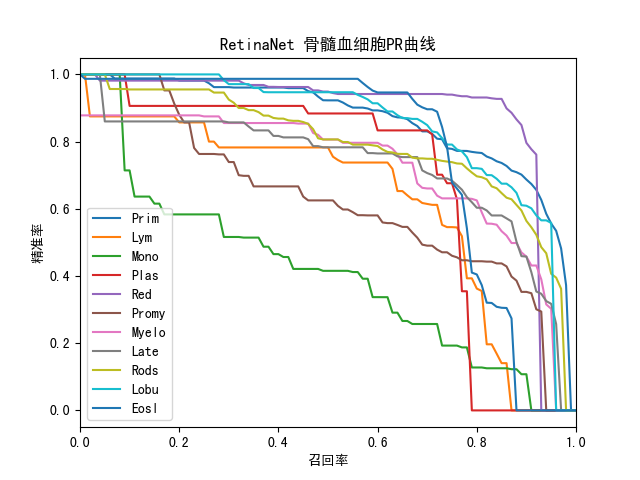
\includegraphics[width=1.0\linewidth, height=0.75\linewidth]{PR_3.png}
    \caption{RetinaNet网络PR曲线}
  \end{subfigure}
  \centering
  \begin{subfigure}{0.48\linewidth}
    \centering
    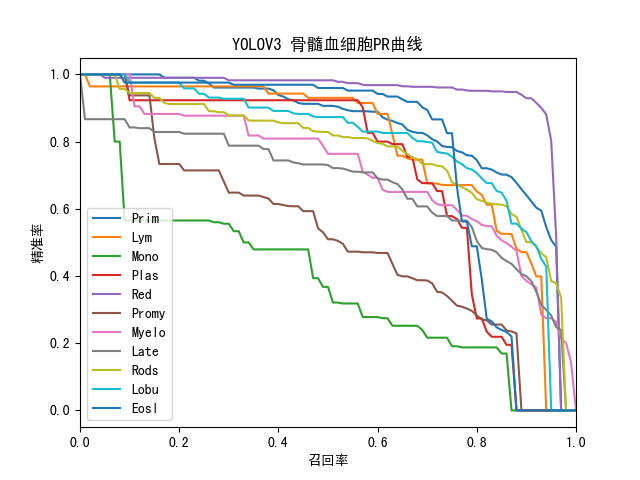
\includegraphics[width=1.0\linewidth, height=0.75\linewidth]{PR_4.png}
    \caption{YOLOV3网络PR曲线}
  \end{subfigure}
	\caption{四种检测网络的PR曲线}
	\label{fig:pr_curve}
\end{figure}

为了进一步直观了解网络的检测性能,我们将检测框进行可视化绘制,如图$~\ref{fig:detect_result}$所示,图中仅展示置信度大于0.6的检测框结果。
图中(a)为血细胞人工标注的结果,(b)-(e)为网络检测的结果。从中我们可以看出原始细胞与嗜中性中幼粒细胞易发生混淆,在第二列图像中,只有Cascade-RCNN网络检测正确,Faster-RCNN与RetianNet
均出现了虚警框。对于第四列图像中的破碎细胞,只有RetinaNet将其识别为背景,而其他网络均出现了虚警。实验结果表明,四种目标检测网络可以有效的检测并识别图像中的骨髓血细胞,
但识别的准确率有待提升。

\begin{figure}[htbp]
	\centering
	\begin{subfigure}{0.9\linewidth}
		\centering
		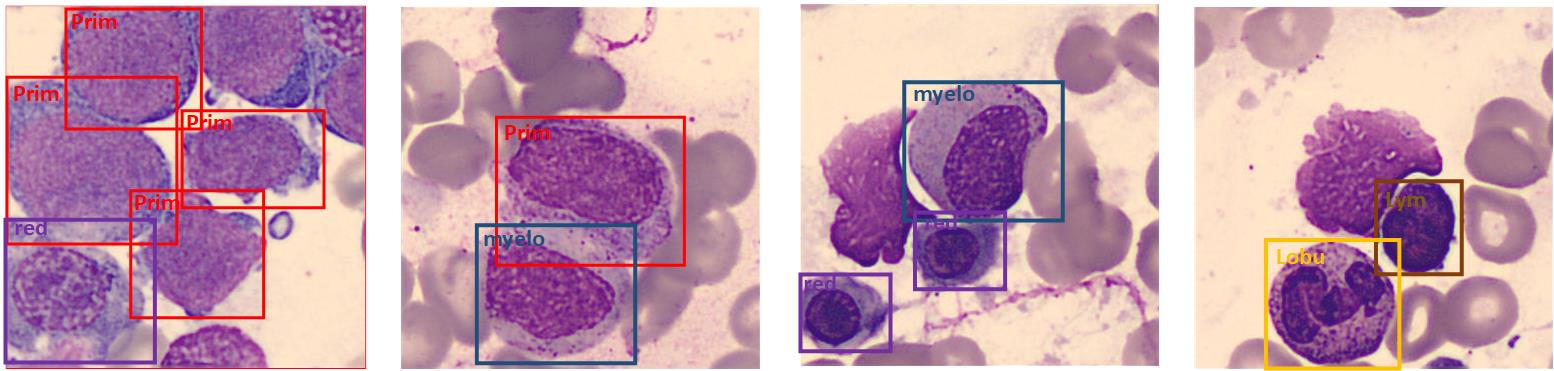
\includegraphics[width=1.0\linewidth, height=0.25\linewidth]{detect_result/gt.jpg}
    \caption{真实标注}
	\end{subfigure}
	\centering
	\begin{subfigure}{0.9\linewidth}
		\centering
		\includegraphics[width=1.0\linewidth, height=0.25\linewidth]{detect_result/faster_rcnn.jpg}
    \caption{Faster-RCNN检测结果}
	\end{subfigure}
	\centering
	\begin{subfigure}{0.9\linewidth}
		\centering
		\includegraphics[width=1.0\linewidth, height=0.25\linewidth]{detect_result/cascade.jpg}
    \caption{Cascade-RCNN检测结果}
	\end{subfigure}
	\centering
	\begin{subfigure}{0.9\linewidth}
		\centering
		\includegraphics[width=1.0\linewidth, height=0.25\linewidth]{detect_result/retinanet.jpg}
    \caption{RetinaNet检测结果}
	\end{subfigure}
	\centering
  \begin{subfigure}{0.9\linewidth}
		\centering
		\includegraphics[width=1.0\linewidth, height=0.25\linewidth]{detect_result/YOLOV3.jpg}
    \caption{YOLOV3检测结果}
	\end{subfigure}
	\caption{四种检测网络的可视化检测结果}
	\label{fig:detect_result}
\end{figure}

综合考虑计算量,参数量与检测精度等因素,我们选择性能较为优异RetinaNet作为基线模型,并基于骨髓血细胞特性对RetinaNet进行改进。

\subsubsection{检测网络与检测识别网络性能对比}

骨髓血细胞检测识别网络需要给出骨髓血细胞的位置与类别,检测网络只需要进行前景检测输出血细胞的位置信息。
我们以RetinaNet单阶段网络作为基线模型,对比了检测网络与检测识别网络在特征图与混淆矩阵上的差异。

骨髓血细胞检测识别的混淆矩阵的定义如下,首先对网络输出的检测框
按照分类置信度进行过滤,只有分类置信度大于阈值的检测框才参与混淆矩阵的计算,然后
基于IOU与标签信息来衡量检测结果是否正确。RetinaNet检测识别网络在score(分类置信度) > 0.3、IOU=0.5条件下的混淆矩阵如图~\ref{fig:det_confusion}(a)所示。
各个类别的召回率与精确率如表~\ref{table:cell_cls}所示。单核细胞(Mono)、杆状核细胞(Rods)与嗜酸性粒细胞(Eosl)
存在比较严重的漏检的问题,召回率小于0.5。嗜中性中幼粒细胞(myelo)与嗜中性晚幼粒细胞(Late)的识准确正确率较差。
检测识别网络平均的检测正确率只有0.581。
RetinaNet检测网络在score(分类置信度) > 0.95、IOU=0.5条件下的混淆矩阵如图~\ref{fig:det_confusion}(b)所示, 骨髓血细胞的召回率0.964,正确率为0.934。
检测网络在$IOU=0.75$条件下的平均精度(AP)为0.942。实验结果表明,在仅做检测后,骨髓血细胞召回率与准确率极高,可以满足实际应用需求。

\begin{table}   
  \caption{RetinaNet网络各类别的准确率与召回率}      
  \centering    
  \label{table:cell_cls}
  \resizebox{0.8\linewidth}{!}{ 
  \begin{tabular}{ccccccc}     
    \hline    
     & prim & lym & mono &  plas & red & promy    \\ 
    \hline      
    Precision    & 0.644 & 0.621 & 0.553 & 0.783 & 0.787 & 0.512  \\      
    Recall       & 0.780 & 0.682 & 0.236 & 0.591 & 0.888 & 0.454 \\      
    \hline         
  \end{tabular} 
  }
  \centering  
  \resizebox{0.8\linewidth}{!}{ 
  \begin{tabular}{ccccccc}                 
     & myelo  & late & rods & lobu &  eosl & 平均 \\          
    \hline          
    Precision    & 0.448 & 0.439 & 0.778 & 0.715 & 0.857 &  0.581   \\      
    Recall       & 0.646 & 0.506 & 0.319 & 0.672 & 0.505 &   \\       
    \hline            
  \end{tabular} 
}  
\end{table}

\begin{figure}[htbp]                  
  \centering                   
	\begin{subfigure}{0.48\linewidth}
		\centering
    \includegraphics[width=1.0\linewidth, height=0.8\linewidth]{det_confusion.png}                   
    \caption{RetinaNet检测识别混淆矩阵}
	\end{subfigure}
	\begin{subfigure}{0.48\linewidth}
		\centering
		\includegraphics[width=1.0\linewidth, height=0.8\linewidth]{det_confusion1.png}
    \caption{RetianNet检测混淆矩阵}
	\end{subfigure}
  \caption{RetinaNet检测识别与检测网络的混淆矩阵}                   
  \label{fig:det_confusion}      
\end{figure}   

检测网络与检测识别网络骨干网络输出的均值特征图如图所示,第一行为检测网络骨干网络在第$2\sim 5$阶段输出的特征图,第二行为检测识别网络输出的特征图。
从图中可以发现检测网络特征图主要关注细胞的边缘信息,而检测识别网络需要关注细胞核、细胞质等全局信息。
我们认为在检测识别网络中,识别任务的难度要远高于坐标回归检测任务。识别任务需要提取精细、丰富的全局特征,
坐标回归任务只需关注中心、边缘等局部特征。两类任务虽然在头部由不同的分支进行学习,但是共享骨干网络提取的特征,
由于任务之间可能存在相互干扰,梯度更新方向不一致,导致骨干网络难以对精细分类特征进行学习,因此识别识别效果较差。

\begin{figure}[htbp]                     
  \centering                      
  \includegraphics[width=0.95\linewidth]{features.jpg}                      
  \caption{检测网络与检测识别网络特征图对比}                      
  \label{fig:feature}       
\end{figure}   

 由于检测识别一体化的网络效果较差,不能满足实际应用的需求。因此,我们先用目标检测网络进行血细胞前景检测与坐标回归,再将血细胞裁剪为切片,
 然后使用血细胞识别网络进行识别。通过将检测任务与识别任务解耦来提高血细胞分类计数任务的准确性。

\section{小结}

针对骨髓血细胞的检测,本章首先分析对比了单双阶段目标检测网络的差异,然后评估了不同
检测网络在骨髓血细胞数据集上的检测精度、计算量与速度等性能。实验结果表明RetinaNet单阶段网络
在速度与精度上要优于其他检目标检测网络,因此我们选择将其作为骨髓血细胞检测的基线模型。此外我们对比了检测网络与
检测识别网络在特征提取与识别准确率上的差异, 实验结果表明检测识别网络的输出类别置信度较低,平均识别正确率只有58.1\%,
易发生漏检与误检。检测网络的平均精度达到了94.2\%,网络检测的准确率与召回率都有大幅提升。
因此我们确定了先检测再识别的骨髓血细胞处理流程,即先使用检测网络定位到血细胞的位置,然后剪切为血细胞切片,
再输入到识别网络中进行分类。





\chapter{基于改进的RetianNet骨髓血细胞检测网络}
\section{引言}

第三章中,我们对比了多个单阶段与双阶段检测网络在骨髓血细胞数据上的性能,综合考虑计算量,参数量与检测精度等因素,
我们选择将性能优异的RetinaNet作为基线模型。此外我们确定了先检测再识别的骨髓血细胞处理流程,即检测网络只需要进行
对血细胞进行前景检测与坐标回归。在RetianNet基线模型中,尽管模型的检测精度已经很高,但仍然存在着漏检、密集与重叠的血细胞区域
边界检测错误等问题,如图~\ref{fig:detect_problem}所示。

骨髓血细胞检测主要有如下三个难点:(1)相比外周血红细胞、白细胞、血小板三类血细胞检测,骨髓血细胞种类繁多、
形态丰富,尺寸大小不一。(2)在骨髓涂片制作过程中,由于染色剂与光照条件的变化,多个批次的数据存在着色彩差异。此外图像
背景复杂,存在较多成熟红细胞的干扰。(3)对于骨髓细胞增生活跃的切片,存在大量血细胞密集堆叠,边缘黏连,易导致漏检、错检等问题。
因此精准检测到骨髓血细胞是一项十分具有挑战性的课题。

针对上述难点与基线模型中存在的问题,本章提出了一种改进RetinaNet网络。该方法中,我们提出了一种基于全局注意力的自底向上的路径聚合网络结构,
缩短了底层与顶层特征之间的信息传递路径,提升网络对位置特征的提取能力。此外探究了不同标签分配策略对检测性能的影响,
提出基于最优输运的标签策略用于密集区域的血细胞的标签分配,避免了模糊分配样本的出现,提高网络对血细胞的召回能力。
% 最后我们比较了空洞卷积、深度可分离卷积、可变形卷积等卷积网络,以期实现速度与检测精度的更优平衡。
在骨髓血细胞数据集上的实验结果表明,本文提出的改进方法在检测准确率上有较大的提升,达到了较为先进的性能。

\begin{figure}[htbp]                     
  \centering                      
  \includegraphics[width=0.7\linewidth]{detect_problem.jpg}                      
  \caption{RetinaNet基线模型检测错误示例}                      
  \label{fig:detect_problem}       
\end{figure}  

\section{改进的RetinaNet骨髓血细胞检测网络}
本章提出的改进RetinaNet网络结构如图~\ref{fig:improved_retinanet}所示,整体网络结构基于第三章的RetinaNet基线模型进行改进。骨干网络为
ResNet50用于图像特征提取,特征金字塔结构用于多尺度特征提取。锚框的尺寸、数量与分类回归网络结果与基线模型相同。
为了提高网络检测的精度,我们在特征金字塔后引入了自底向上的路径聚合模块,该模块基于全局注意力将更浅层的特征与FPN深层的进行融合,
提升网络定位特征的表达能力,此外我们引入了可变形卷积、空洞卷积等卷积模块。在训练过程中,我们使用基于最优输运的策略进行标签分配。
下面各个小节将详细介绍我们的改进点。
\begin{figure}[htbp]                     
  \centering                      
  \includegraphics[width=0.95\linewidth]{improved_retinanet.png}                      
  \caption{改进的RetinaNet网络结构示意图}                      
  \label{fig:improved_retinanet}       
\end{figure}  

\subsection{基于全局注意的路径聚合网络}
ResNet50骨干网络提取了不同层级与尺度的特征图,高层次的特征图表达目标的抽象语义信息,低层次的特征图表达局部的纹理与模式信息,因此引入了
特征金字塔网络,增加自上而下的路径来传播语义强的特征,从而增强所有层次特征的分类能力。在骨髓血细胞检测任务中,我们更加关注网络对于血细胞的
定位的准确性,这些定位信息主要存在浅层特征图的边缘、纹理信息中。我们构建了自底向上的路径聚合网络,将浅层的特征与特征金字塔深层的特征图
进行融合,通过特征直连缩短了底层到顶层特征之间的信息传递路径。原始结构中底层到顶层需要需要约50层网络,如图~\ref{fig:panet}红线所示。自下而上的路径聚合网络引入了
特征直连,从底层到顶层的路径只有不到10层,如图~\ref{fig:panet}绿线所示,该路径使得浅层的纹理等高分辨定位信息可以更有效的传递到顶层,
提升网络定位特征的表达能力。
\begin{figure}[htbp]                     
  \centering                      
  \includegraphics[width=0.75\linewidth]{panet.jpg}                      
  \caption{路径聚合网络结构示意图}                      
  \label{fig:panet}       
\end{figure}  

图中${C_2, C_3, C_4, C_5}$为ResNet50骨干网络不同阶段生成的特征图,${P_2, P_3, P_4, P_5}$为特征金字塔生成的不同级别的特征图。
自底向上的路径聚合网络从最底层的P2特征图开始,通过步长为2的卷积进行下采样并与高层的特征融合后生成新的特征图${N_2, N_3, N_4, N_5}$。
路径构建模块中使用了全局通道注意力机制,使用全局上下文信息的高层次特征指导浅层特征的筛选,该结构如图~\ref{fig:gau}所示。

\begin{figure}[htbp]                     
  \centering                      
  \includegraphics[width=0.95\linewidth]{gau.jpg}                      
  \caption{全局注意力模块}                      
  \label{fig:gau}       
\end{figure}  

全局注意力模块的输入分别是路径聚合网络的低层级的特征图$N_i(H_1 \times W_1 \times C_1)$与特征金字塔的高层级特征图
$P_{i + 1}(H_2 \times W_2 \times C_2)$,输出新的特征图$N_{i + 1}$。首先对特征图$N_i$经过$3\times 3$、步长为2
的卷积层降低特征图的尺寸得到$I^{\prime}_i({H_2} \times {W_2} \times {C_2})$。对高层级的特征图$P_{i + 1}$进行全局
平均池化,每个通道压缩为一个值得到C维向量$z(1 \times 1 \times {C_2})$,如式~\ref{eq:squeeze}所示:
\begin{equation}   
  \mathbf{z} = {{\bf{F}}_{sq}}\left( {{{\bf{P}}_{i + 1}}} \right) = \frac{1}{{H \times W}}\sum\limits_{i = 1}^H {\sum\limits_{j = 1}^W {{{\bf{P}}_{i + 1}}} } (i,j)
  \label{eq:squeeze} 
\end{equation}

然后使用两层全连接结构来全局建模通道之间的依赖关系,第一层全连接的输出使用ReLU激活函数,第二层使用Sigmoid激活函数,得到权重
$\mathbf{w}(1 \times 1 \times {C_2})$,如式~\ref{eq:excitation}所示。
\begin{equation}   
  {\bf{w}} = {{\bf{F}}_{ex}}({\bf{z}},{\bf{W}}) = \sigma (g({\bf{z}},{\bf{W}})) = \sigma \left( {{{\bf{W}}_2}\delta \left( {{{\bf{W}}_1}{\bf{z}}} \right)} \right)
  \label{eq:excitation} 
\end{equation}

将权重向量$\mathbf{w}$与和特征$I^{\prime}_i({H_2} \times {W_2} \times {C_2})$按通道点乘得到加权后的特征$I^{\prime \prime}_i({H_2} \times {W_2} \times {C_2})$,
如式~\ref{eq:scale}所示。
\begin{equation}   
  {\bf{I}}_i^{\prime \prime } = {{\bf{F}}_{{\rm{scale }}}}\left( {{\bf{I}}_i^\prime ,{\bf{w}}} \right) = {w_c}I^\prime_{ic}
  \label{eq:scale} 
\end{equation}

将$\bf{I}_i^{\prime \prime}$与$P_{i + 1}$逐元素相加后再经过一个$3\times3$卷积层后得到路径聚合网络的下一层特征图$N_{i + 1}$。
不断迭代上述过程,直到生成$N_5$特征图为止。最终在融合后新的特征图$N_2, N_3, N_4, N_5$上进行区域提取与坐标回归。
anchor生成与分类回归结构与RetianNet相同,在第三章已进行详细解释。

\subsection{IOU预测分支}
RetinaNet在预测阶段会生成密集的检测框,这些检测框会按照置信度高低进行非极大值抑制(NMS),去除重复的检测框。上述NMS方式默认了一种假设,就是
置信度高的锚框定位也会更加精确。
\begin{figure}[htbp]
	\centering
  \begin{subfigure}{0.35\linewidth}
    \centering
    \includegraphics[width=0.95\linewidth, height=0.95\linewidth]{cell1.jpg}
    \caption{}
  \end{subfigure}
	\centering
	\begin{subfigure}{0.35\linewidth}
		\centering
		\includegraphics[width=0.95\linewidth, height=0.95\linewidth]{cell2.jpg}
    \caption{}
	\end{subfigure}
  \caption{置信度高但交并比低的错误检测示例}
	\label{fig:detect_err}
\end{figure}
但是部分细胞例如杆状核细胞不服从中心分布,因此分类与归回这两种任务不一定严格正相关\cite{he2019bounding},如图~\ref{fig:detect_err}所示,
图中(a)无论置信度分数高低,血细胞检测框的坐标都不准确,(b)中置信度分数更高的检测框右侧与上侧的边界都是不准确的,而置信度较低的检测框边界正确。


我们认为需要将检测框的定位质量也纳入到非极大值抑制的考量当中,在挑选分数最大的检测框时同时考虑置信度与交并比。但是在预测阶段,
没有目标真实的坐标信息,因此无法使用交并比来判断每个检测框定位质量的好坏。我们在网络的定位部分额外扩展出了一个子分支来预测每一个锚框
可能对应真实框的交并比。该分支与定位分支共享特征图信息,使用一个卷积层对于每个锚框输出一个标量值,然后使用Sigmoid激活函数进行激活去得到
一个零一之间的交并比信息,修改后的网络结构如图~\ref{fig:cls_reg}所示。图中(a)为RetinaNet的分类回归分支网络结构。图(b)中在回归分支
加入了一个额外的卷积层,去预测交并比信息。
\begin{figure}[htbp]
  \centering
	\begin{subfigure}{0.45\linewidth}
		\centering
		\includegraphics[width=0.95\linewidth, height=0.85\linewidth]{cls_reg1.jpg}
    \caption{}
	\end{subfigure}
  \centering
	\begin{subfigure}{0.45\linewidth}
		\centering
		\includegraphics[width=0.95\linewidth, height=0.85\linewidth]{cls_reg2.jpg}
    \caption{}
	\end{subfigure}
  \caption{交并比预测分支结构}
	\label{fig:cls_reg}
\end{figure}

在训练过程,我们优化的目标有分类,坐标回归与交并比,损失函数如式~\ref{eq:loss_all}所示,其中${{L_{IoU}}(io{u_i},io{u_i}^*)}$定义为预测IoU和真实IoU之间的二元交叉熵损失。
\begin{equation}   
  Loss = \sum\limits_i {{L_{cls}}} \left( {{p_i},p_i^*} \right) + {\lambda _1}\sum\limits_i {p_i^*} {L_{reg}}\left( {{t_i},t_i^*} \right) + {\lambda _2}\sum\limits_i {{L_{IoU}}(io{u_i},io{u_i}^*)} 
  \label{eq:loss_all} 
\end{equation}




\subsection{训练标签分配策略}
  在目标检测网络训练过程中,标签分配(Label Assignment)是非常重要的一个流程。其目的是将训练样本划分为正负样本,并分配分类与回归的目标,
  计算其与真值之间的损失来监督训练。标签分配方式为网络训练提供了判别性的监督信号,决定了网络学习与收敛的方向,直接影响模型性能的好坏。
  本节介绍了我们训练过程中采用的不同标签分配策略,根据样本标签分配的正负权重设计,可以将这些方法划分为硬标签分配方法与软标签分配方法。

\subsubsection{硬标签分配策略}
硬标签分配策略假设每个锚框非正即负,若$w_{pos}, w_{neg}$分别表示样本属于正负样本的权重,则硬标签划分可以表示为
$w_{\text {pos }}, w_{n e g} \in\{0,1\}$且$w_{\text {pos }} +  w_{n e g} = 1$。这类方法的核心思想是找到一个最优划分
边界,将锚框分割为正样本集合与负样本集合。边界划分规则可以分为静态规则与动态规则这两类。

\subsubsection{最大交并比}
RetinaNet与Faster-RCNN等网络采用的是最常用的基于交并比最大化的标签分配策略(MaxIouAssigner)。
该方法主要由以下的几个步骤:(1)初始化,将正样本集合$P$、负样本集合$N$设置为空集,将所有锚框设置为忽略样本;
(2)计算多尺度特征图上所有锚框与所有真实框之间的交并比;(3)获取每个锚框交并比最大的GT框,如果交并比大于正样本阈值
(pos\_thres),则设置为正样本。如果小于负样本阈值(neg\_thres),则设置为负样本。(4)如果GT框没有被锚框匹配到,
则获得与GT框IOU最大的锚框,如果大于最小的正样本阈值,则将该锚框设置为正样本。

最大交并比标签分配策略是静态预先定义的标签分配方式。骨髓血细胞形状多变,比如杆状核粒细胞,通常呈现出U型,这导致目标的中心点
通常为背景,并不能代表这个目标,而按照最大交并比的方式会被判定为正样本,导致网络的性能较差。

\subsubsection{自适应样本选择}
自适应样本选择(Adaptive Training Sample Selection,ATSS)方法基于L2距离与交并比动态计算分割阈值,是一种自适应划分
目标正负样本的标签分配策略。具体步骤如下:(1)对于网络输出的多个不同尺度特征图,在每个特征图上计算锚框中心坐标与目标中心
坐标的$L_2$距离,选取$K$个$L_2$距离最小的锚框作为候选的正样本,如果有$L$个层级的特征图,那么可以得到$K \times L$个候选正样本
。(2)计算每个候选正样本与目标真实框的交并比,得到一组交并比的数据。计算这组交并比的均值$m_g$与标准差$v_g$,将均值与标准差
相加,得到交并比的分割阈值$t_g = m_g + v_g$(3)在每个层级的特征图的候选正样本中根据阈值,选择真正的正样本加入正样本集合中进行训练。

\begin{figure}[htbp]
	\centering
  \begin{subfigure}{0.48\linewidth}
    \centering
    \includegraphics[width=1.0\linewidth, height=0.56\linewidth]{atss1.jpg}
    \caption{}
  \end{subfigure}
  \begin{subfigure}{0.48\linewidth}
    \centering
    \includegraphics[width=1.0\linewidth, height=0.56\linewidth]{atss2.jpg}
    \caption{}
  \end{subfigure}
\caption{自适应样本选择阈值计算示意图}
	\label{fig:atss}
\end{figure}

图~\ref{fig:atss}为ATSS自适应计算阈值的示意图,柱状图的横坐标表示不同层级特征图,纵轴为交并比。柱子上的数字表示这个层级特征图上
目标与最近$K$个锚框交并比的均值。均值$m_g$代表锚框与目标真实框的匹配程度,如果$m_g$比较大,则候选正样本的质量都很好,
可以适当提高阈值来挑选更好正样本。均值低则应当降低分割阈值。标准差$v_g$表示特征层次锚框与目标真实框的匹配程度。如果标准差比较高,
则高质量的锚框集中在某一个层级的特征图中,应该提高阈值从最匹配的层级去挑选正样本。标准差比较低,说明所有层级的锚框匹配度都比较高,
可以设置一个比较低的阈值广泛的从多个层级的特征图中选取。

\subsubsection{概率标签分配}
概率标签分配(Probabilistic Anchor Assignment,PAA)将锚框的得分数视为概率分布,并通过最大似然来估计分布参数,然后自适应的计算分割
阈值,来选取正负样本。锚框的分数用来衡量其与真实框的相似性,包括了分类得分与定位得分。分类得分是分类分支输出的置信度${P_i}(cls|\theta )$,定位得分为
预测框与真实框之间的交并比${\rm{IOU}}(f(a|\theta ),g)$,为平衡这两种得分的权重,引入$\lambda$参数。锚框得分如式~\ref{eq:score}所示:
\begin{equation}   
  S = {P_i}(cls|\theta ) \times {\rm{IOU}}{(f(a|\theta ),g)^\lambda } 
  \label{eq:score} 
\end{equation}

锚框可以分为正样本、负样本两组,因此可以使用双峰混合高斯分布来建模锚框的分数分布,如式~\ref{eq:gmm}所示。
\begin{equation}   
  P(a|g,\theta ) = {\phi _1}{\cal N}(a;{\mu _1},{\sigma _1}) + {\phi _2}{\cal N}(a;{\mu _2},{\sigma _2})
  \label{eq:gmm} 
\end{equation}

然后根据最大期望算法(Expectation-Maximization,EM)使得似然最大化。首先对参数$\phi_i, \mu_i, \sigma_i$进行随机初始化,
在E步中计算Q函数如式~\ref{eq:e_step}所示,式中$x_{1}, x_{2}, \ldots, x_{n}$为锚框的得分。
\begin{equation}   
  Q_{i}\left(z^{(i)}=k\right)=\frac{\phi_{k} \cdot \frac{1}{\sqrt{2 \pi} \sigma_{k}} \exp \left[-\frac{\left(x^{(i)}-\mu_{k}\right)^{2}}{2 \sigma_{k}^{2}}\right]}{\sum_{k=1}^{K} \phi_{k} \cdot \frac{1}{\sqrt{2 \pi} \sigma_{k}} \exp \left[-\frac{\left(x^{(i)}-\mu_{k}\right)^{2}}{2 \sigma_{k}^{2}}\right]}
  \label{eq:e_step} 
\end{equation}

在M步中根据式~\ref{eq:m_step}计算混合高斯分布的参数$\phi_1,\phi_2,\mu_1,\sigma_1,\mu_2,\sigma_2$。

概率标签分配的具体步骤如下:对于每个真实框,根据网络输出的置信度与坐标计算每个锚框的得分,在每个尺度的特征度选择K个得分最高的锚框。
采用最大期望算法去估计这组锚框的双峰高斯分布参数,找到两个最高峰对应横坐标的分数$s_1,s_2$,其中$s_1 < s_2$。(3)将得分低于$s_1$的锚框
作为负样本。得分位于$s_1$与$s_2$之间的锚框划分为忽略样本,得分大于$s_2$的锚框作为正样本。最后那些没有参与分配的锚框均视为负样本。

\begin{equation}   
  \begin{aligned} \mu_{k} & =\frac{\sum_{i=1}^{N} Q_{k}^{(i)} x^{(i)}}{N_{k}} \\ 
    \sigma_{k} & =\frac{\sum_{i=1}^{N} Q_{k}^{(i)}\left(x^{(i)}-\mu_{(k)}\right)\left(x^{(i)}-\mu_{k}\right)^{T}}{N_{k}} \\ 
    \phi_{k} & =\frac{\sum_{i=1}^{N} Q_{k}^{(i)}}{N} \\ 
    N_{k} & =\sum Q_{k}^{N} Q_{k}^{(i)} 
  \end{aligned}
  \label{eq:m_step} 
\end{equation}

\subsubsection{最优输运标签分配}
最优输运标签分配将目标检测中的标签分配问题建模为
将标签从真实框输运到锚框代价最小的最优输运策略(Optimal Transport)问题,如图~\ref{fig:ota}所示。

最优输运问题的定义如下:假设有m个供应商与n个需求方,其中第$i$
个供应商有$a_i$单元的货物,第$j$个需求方需要$b_j$个单元的货物。每个单元的货物从第$i$个供应商运输到第$j$个的需求方的输运代价是$C_{ij}$。
最优输运的目标是找到一种输运计划$\mathbf{P}^{*}=\left\{P_{i, j} \mid i=1,2, \ldots m, j=1,2, \ldots n\right\}$将供应商的货物全部运输到需求方,
并使得运输的代价最小,其中$P_{i, j}$表示第$i$个供应商运输到第$j$个的需求方单元货物的数量。

\begin{figure}[htbp]                     
  \centering                      
  \includegraphics[width=0.95\linewidth]{ota.jpg}                      
  \caption{基于最优输运的标签分配策略}                      
  \label{fig:ota}       
\end{figure}  

最优输运的优化目标如式~\ref{eq:ota}所示:
\begin{equation}   
  \min _{\mathbf{P}} \sum_{i=1}^{m} \sum_{j=1}^{n} C_{i j} P_{i j} \quad P_{i j} \geq 0,i=1,2, \ldots m, j=1,2, \ldots n .
  \label{eq:ota} 
\end{equation}

其中第i的供应商输出的数量等于$s_i$,即$ \sum_{j=1}^{n} P_{i j}=a_{i}$。第j个需求方接收的数量等于$b_j$,即$\sum_{i=1}^{m} P_{i j}=b_{j}$。
供应商供应的数量等于需求方接收的数量$\sum_{i=1}^{m} a_{i}=\sum_{j=1}^{n} b_{j}$。

最优输运问题可以在多项式的时间复杂度内,通过Sinkhorn快速迭代的方法进行求解。该方法的思想源于交叉熵与对偶问题,定义$\mathbf{H}(\mathbf{P}) \stackrel{\text { def. }}{=} -\sum_{i, j} \mathbf{P}_{i, j}\left(\log \left(\mathbf{P}_{i, j}\right)-1\right)$
上述问题添加了拉格朗日算子和扰动项的形式如式~\ref{eq:ota_1}所示:
\begin{equation}   
  {\cal E}({\bf{P}},{\bf{f}},{\bf{g}}) = \sum\limits_{i = 1}^m {\sum\limits_{j = 1}^n {{{C}_{ij}}} } {{P}_{ij}} - \varepsilon {\bf{H}}({\bf{P}}) + {f_j}\left( {\sum\limits_{i = 1}^m {P_{ij}}  - {b_j}} \right) + {g_i}\left( {\sum\limits_{j = 1}^n {P_{ij}}  - {a_i}} \right)
  \label{eq:ota_1} 
\end{equation}

其中$\varepsilon$是一个常量超参数,控制熵正则化项的强度,实验中设置为0.1,$f_{j}(j=1,2, \ldots n)$与$g_{i}(i=1,2, \ldots, m)$是拉格朗日乘子。
通过使得目标函数导数等于零求得最优的输运策略如式~\ref{eq:ota_2}所示:
\begin{equation}   
  \frac{\partial \mathcal{E}(\mathbf{P}, \mathbf{f}, \mathbf{g})}{\partial P_{i, j}}=C_{i, j}+\varepsilon \log \left(P_{i, j}\right)-f_{j}-g_{i}=0
  \label{eq:ota_2} 
\end{equation}

因此最优输运策略为$\mathbf{P}^{*}$如式~\ref{eq:ota_3}所示:
\begin{equation}   
  P_{ij}^* = \exp \left( { - \frac{{{f_j}}}{\varepsilon }} \right)\exp \left( { - \frac{{{C_{ij}}}}{\varepsilon }} \right) \exp \left( { - \frac{{{g_i}}}{\varepsilon }} \right)
  \label{eq:ota_3} 
\end{equation}

令$s_j=\exp \left( { - \frac{{{f_j}}}{\varepsilon }} \right)$, $U_{ij}=\exp \left( { - \frac{{{C_{ij}}}}{\varepsilon }} \right)$,$t_i=\exp \left( { - \frac{{{g_i}}}{\varepsilon }} \right)$
上述变量满足如式~\ref{eq:ota_4}的约束关系:
\begin{equation}   
  \begin{array}{l}
  \sum_{i} P_{i j}=s_{j}\left(\sum_{i} U_{i j} t_{i}\right)=b_{j} \\
  \sum_{j} P_{i j}=\left(s_{j} \sum_{i} U_{i j}\right) t_{i}=a_{i}
  \end{array}
  \label{eq:ota_4} 
\end{equation}

上式的约束关系需要同时满足,因此$t_i$与$s_j$的交替迭代公式如下:
\begin{equation}   
  s_j^{l + 1} = \frac{{{b_j}}}{{\sum\limits_i {{U_{ij}}} t_i^l}},\quad t_i^{l + 1} = \frac{{{a_i}}}{{\sum\limits_j {{U_{ij}}} s_j^{l + 1}}}
  \label{eq:ota_5} 
\end{equation}

在目标检测的背景下,假设一张图片中有$m$个真实框,检测网络所有的FPN层总共输出了$n$个锚框。将真实框
视为供应商,可以为$k$个锚框提供正样本的标签,等价于有$k$个单元的货物$\text { i.e., } a_{i}=k, i=1,2, \ldots, m$。
每个锚框视为需求方,需要一个标签$\text { i.e., } b_{j}=1, j=1,2, \ldots, n$。此外引入一个背景供应商,来为锚框提供
负样本标签,数量为$n - m \times k$。

将正样本标签从某一个真实框$gt_{i}$输运到一个锚框$anchor_j$的代价定义为分类与回归的加权损失,如式~\ref{eq:ota_cost_fg}所示:
\begin{equation}   
  C_{ij}^{fg} = {L_{cls}}\left( {p_i^*,p_j^{cls}(\theta )} \right) + \lambda {L_{reg}}\left( {t_i^*,t_j^{box}(\theta )} \right)
  \label{eq:ota_cost_fg} 
\end{equation}

其中$\theta$代表模型参数,$p_j^{cls}(\theta )$与$t_j^{box}(\theta )$分别代表模型预测的分类得分与坐标回归值。
$p_i^*$与$t_i^*$代表了真实类别与坐标。$L_{cls}$与$L_{reg}$为交叉熵损失函数与GIOU损失函数。

背景供应商将一个负样本标签传递到锚框的花费为分类损失,如下式所示:
\begin{equation}   
  C_j^{bg} = {L_{cls}}\left( {\Phi ,p_j^{cls}(\theta )} \right)
  \label{eq:ota_cost_bg} 
\end{equation}

在定义好花费矩阵后,最优输运的策略$\mathbf{P^*}$可以可以通过Sinkhorn-Knopp迭代算法进行求解。每个anchor的标签
为最大的标签所对应的供应商类别。算法流程如算法~\ref{alg:alg_ota}所示。

\renewcommand{\algorithmicrequire}{\textbf{输入:}\unskip}
\renewcommand{\algorithmicensure}{\textbf{输出:}\unskip}

\begin{algorithm}[h]
  \caption{最优输运标签分配} % 名称
  \label{alg:alg_ota}
  \begin{algorithmic}[1]
    \REQUIRE
      ~\\
      $I$: 输入图像            \\
      $A$: 网络输出的一组锚框   \\
      $G$: 图像中目标真实框标注 \\
      $\varepsilon$: Sinkhorn-Knopp迭代熵正则化项 \\
      $T$: Sinkhorn-Knopp迭代次数 \\
      $\lambda$: 式~\ref{eq:ota_cost_fg}中的平衡因子 
    \ENSURE
      ~\\
      $\mathbf{P^*}$标签最优输运策略
      \STATE set $m = |G|$, $n = |A|$;
      \STATE 网络前向计算每个锚框的分数与坐标$P^{cls}, P^{box}$
      \STATE 动态计算每个GT框的$a_i$
      \STATE 计算得到背景供应商的标签数量$a_{m + 1} = n-\sum_{i=1}^{m} a_{i}$
      \STATE $b_j(j = 1, 2 \dots n)$使用1初始化
      \STATE 前景分类损失$C_{ij}^{cls} = FocalLoss(P_{j}^{cls}, G_{i}^{cls})$
      \STATE 前景回归损失$C_{ij}^{reg} = IoULoss{P_{j}^{box}, G_{i}^{box}}$
      \STATE 背景花费$C_{bg}^{cls} = FocalLoss(P_{j}^{cls}, \Phi)$
      \STATE 前景花费$C_{fg} = C^{cls} + \lambda C^{reg}$
      \STATE 计算最终的花费矩阵将$C_{bg}$拼接到$C_{fg}$的最后一行
      \STATE 对$s^0, t^0$进行随机初始化
      \FOR {$i = 1$; $i < T$; $i++$ }
        \STATE 计算$s^{l+1}, t^{l+1} \leftarrow \operatorname{SinkhornIter}\left(C, s^{l}, t^{l}, a, b\right)$
     \ENDFOR
      \STATE 根据式~\ref{eq:ota_3}, 计算并返回最优的标签分配策略$\mathbf{P}^*$
  \end{algorithmic}
\end{algorithm}

% \subsubsection{软标签分配策略}
% \subsection{完全动态标签分配}
\subsection{损失函数}

\section{算法实现与实验结果分析}
\subsection{实验环境}
\subsubsection{数据集介绍}

骨髓血细胞图像来自邃蓝智能科技(上海)有限公司合作医院提供,首先采用第2.1小节阐述的主动学习标注策略进行边界框的标注。
我们总共标记了6821张血细胞图像,训练集与测试集按照4:1的比例进行随机划分,训练集包含了5456张图像,测试集包含了1365张图像。
通常每个图像中包含1到10个有核血细胞,数据集总共标记了11352个血细胞,训练集有9065个血细胞,测试集有2287个血细胞。数据集的分布如
表~\ref{table:cell_detect1}所示:

\begin{table}
  \caption{骨髓血细胞检测数据集分布}   
  \centering 
  \label{table:cell_detect1}
  \begin{tabular}{ccccc}
    \toprule[2pt]
    序号 & 类别名  &  类别简写 & 训练集数量 & 测试集数量 \\
    \midrule[1.5pt] 
    1 & 原始细胞 & Prim & 1856 & 467 \\ 
    2 & 淋巴细胞 & Lym & 996 & 226   \\ 
    3 & 单核细胞 & Mono & 206 & 52   \\ 
    4 & 浆细胞 & Plas & 272 & 70   \\ 
    5 & 红细胞 & Red & 1880 & 503   \\ 
    6 & 早幼粒细胞 & Promy & 357 & 107   \\ 
    7 & 嗜中性中幼粒细胞 & Myelo & 701 & 150   \\ 
    8 & 嗜中性晚幼粒细胞 & Late & 503 & 144   \\ 
    9 & 嗜中性杆状核细胞 & Rods & 998 & 241   \\  
    10 & 嗜中分叶核细胞 & Lobu & 821 & 195   \\  
    11 & 嗜酸性粒细胞 & Eosl & 475 & 132   \\  
    \hline
    总计 &   &   & 9065 & 2287 \\
    \bottomrule[2pt]      
  \end{tabular} 
\end{table}

\subsection{实验结果与分析}
\subsubsection{评价指标} 
\subsubsection{实验结果}
\subsubsection{路径聚合网络}
\subsubsection{标签分配策略}
\section{小结}



% \chapter{基于改进Vision Transformer骨髓血细胞检测算法设计与实现}
\section{引言}
% 研究背景,现状 挑战与本文贡献
白血病是一种人体造血系统的恶性肿瘤,在所有恶性肿瘤中占比约5\%,是我国重点防治的十大恶性肿瘤之一。
血细胞形态学检查是白血病诊断常规检查的一部分,各类骨髓血细胞经过染色后呈现出不同的形状、颜色与纹理,
这些细胞由经验丰富的病理专家识别并计数,最终根据FAB标准给出白血病类型的诊断。上述人工镜检的诊断流程存在以下不足,
人工分类计数繁琐费时,诊断结果具有较强的主观性。此外,细胞形态学人才资源紧缺,
培养精通细胞病理诊断的医师要耗费大量的时间。通过研究骨髓血细胞自动化识别技术来辅助临床诊断,可以实现诊断流程的标准化、
快速化与智能化,将医生从繁重的病理工作中解放出来,具有重要的临床意义和广阔的应用前景。

近年来,基于深度学习的方法在医学影像处理领域取得了巨大的成功,
国内外学者纷纷开始探索基于深度学习的血细胞识别方法。基于深度学习的血细胞识别方法不再需要进行复杂的血细胞特征工程
设计,直接将血细胞数据输入网络中进行端到端训练。通过优化损失函数,网络可以自动挖掘数据的潜在特征,并基于这些特征进行
预测,相比于传统识别方法具有更高的识别准确率。根据文献调研,血细胞识别算法主要基于计算机视觉领域的目标识别网络并通过迁移学习进行微调,这些识别
网络包括了ResNext、ResNet与EfficientNet等,在血细胞数据集上获得了很好的识别结果。

骨髓血细胞自动化识别是一项非常具有挑战性的任务,主要存在着以下难点:(1)缺少大规模的骨髓血细胞识别任务数据集,
不同批次的骨髓血细胞存在染色、光照等差异,导致切片图像外观、颜色变化的多样性。
(2)各类骨髓血细胞在人体中的所占比例不同,导致数据集中各个类别样本数量分布不均衡,
数量较少类别的骨髓血细胞难以有效的进行特征学习。
(3)骨髓血细胞种类繁多,例如粒细胞有原始、早幼、中幼与晚幼等阶段,
相邻发育阶段的血细胞在形态上非常类似,骨髓血细胞子类之间差异较小增加了细粒度识别的难度。

针对骨髓血细胞识别过程中的难点,本章提出了一种基于改进Vision Transformer的骨髓血细胞识别方法。
首先,使用第四章提出的改进RetinaNet网络从图像中检测出细胞边界并进行裁剪,去除背景等干扰。
接着,本章提出一种重叠图像块划分方法将裁剪后的图像分割为多个图像块并学习嵌入向量表示。
然后,嵌入向量经过多个编码层进行特征提取。本章基于多头自注意机制提出了稀疏注意力模块,
该模块可以捕捉图像中的辨识性区域,提取图像中的细粒度特征,并将筛选后的特征输入到编码层。
最后,网络输出的分类特征用于骨髓血细胞的识别。在训练过程中,本章采用对比损失进一步增加分类特征的类内一致性与类间差异性。
最后,在邃蓝智能骨髓血细胞数据集与开源的慕尼黑血细胞形态学数据集实验结果表明,
我们提出的方法具有良好的精细分类性能,相比于其他识别方法具有更高的识别准确率

本章内容源自我以第一作者发表的文章《基于改进Vision Transformer的血细胞图像识别方法研究》\cite{SWGC202206005}

\section{改进的Vision Transformer骨髓血细胞识别网络}

本文提出的基于Vision Transformer的骨髓血细胞识别网络框架如图~\ref{fig:vit}所示。
首先将输入的血细胞图像分割为$N$个$P \times P$大小的图像块,接着将图像块线性映射为序列化嵌入向量,
其次加入可学习的分类向量与位置编码信息。然后嵌入向量被输入到多个堆叠的编码模块中进行特征提取。
在最后一层编码模块前,使用辨识性区域选择模块来寻找图像中的区分性像素块并将其对应的隐含特征作为输入。
最后编码器输出的分类特征经过全连接层得到骨髓血细胞的类别概率信息。

\begin{figure}[htbp] 
   \centering   
   \includegraphics[width=0.9\linewidth]{transFG.png}   
   \caption{基于改进Vision Transformer骨髓血细胞识别网络结构}   
   \label{fig:vit} 
\end{figure}  

\subsection{重叠图像块划分}
Vision Transformer模型接收的输入为序列化数据,因此需要将图像划分为图像块并线性映射为序列化向量(token)。
Vision Transformer模型将图像划分成大小为$P \times P$且互不重叠的像素块,但这样划分会破坏图像的局部结构,
例如辨识性区域被划分到两个相邻的图像块中。为避免该问题,本文采用滑动窗的方法来生成有重叠的图像块。
当输入图像的尺寸为$H \times W \times C$、图像块大小为$P$、滑动窗的步长为$S$时,图像将会被划分为$N$个像素块,
其中$N$如式~\ref{eq:embed}所示。
\begin{equation}
  n=n_{h} \times n_{w}=\left\lfloor\frac{h-p}{s}+1\right\rfloor \times\left\lfloor\frac{w-p}{s}+1\right\rfloor
  \label{eq:embed}
\end{equation}

通过滑动窗的方式,两个相邻像素块的重叠面积为$(P-S) \times P$,更好的保留了图像的局部信息。
当$S$越小,局部结构保存的越完整,但会增加序列化向量的数量导致计算开销变大。
综合利弊,在实验中将S的大小设置为$2P/3$。图像划分完成后,需要将2-D的图像块转化为1-D的序列向量,
首先将图像块展平为一组向量$x_{\mathrm{p}} \in \mathbb{R}^{N \times P^{2} \mathrm{C}}$,
然后通过线性变换将其映射到$D$的维度大小。
上述转化在具体实现上等价于对原图像进行$D$个$P \times P \times P^2C$尺寸的卷积核、步长为$2P/3$的卷积操作。
由于嵌入后的向量不包含位置信息,需要加入一个特殊的可学习位置编码。
此外还加入可学习分类向量作为最终的输出特征用于图像分类。
嵌入后的序列数据$\mathbf{z}_{0}$如式~\ref{eq:embed1}所示,其中$\boldsymbol{E}$为投影矩阵、$\boldsymbol{E}_{\mathrm{pos}}$为位置编码、$\boldsymbol{x}_{\text {class }}$为分类向量。
\begin{equation}
    \mathbf{z}_{0}=\left[\boldsymbol{x}_{\text {class }} ; \boldsymbol{x}_{p}^{1} \boldsymbol{E} ; \boldsymbol{x}_{p}^{2} \boldsymbol{E} ; \cdots ; \boldsymbol{x}_{p}^{N} \boldsymbol{E}\right]+\boldsymbol{E}_{\mathrm{pos}}
    \label{eq:embed1}
\end{equation}

图片序列化之为一组向量后,网络需要知道每一个token在序列中的绝对位置,并且不同token之间的相对位置也需要保持一致。因此引入位置编码(Positional Embedding,PE)来
表示token的位置关系。位置编码采用连续有界的正弦、余弦函数来表示位置信息,受到二进制编码的启发,位置编码向量的低位角频率较大,模拟二进制低位0、1的高频交互,
位置编码高位角频率小,对位置$t$的变动不敏感,模拟二进制的高位变化较小。为了可以用线性变换表示相对位置变动,采用正弦与余弦一组的方式对位置编码进行表示。
定义$t$为这个token在序列中的实际位置,$P E_{t} \in \mathbb{R}^{d}$表示这个token的位置编码向量,$P E_{t}^{(i)}$表示位置编码向量中的第i个
元素,$d_{model}$为位置编码的维度,则位置编码$P E_{t} \in \mathbb{R}^{d}$如式~\ref{eq:pos_embed}所示:
\begin{equation}
  P E_{t}^{(i)}=\left\{\begin{array}{l}
  \sin \left(w_{i} t\right), \quad \text { if } k=2 i \\
  \cos \left(w_{i} t\right), \quad \text { if } k=2 i+1
  \end{array}\right.
  \label{eq:pos_embed}
\end{equation}

其中$w_{i}=\frac{1}{10000^{2 i / d_{\text {model }}}}$,$i=0,1,2,3, \ldots, \frac{d_{\text {model }}}{2}-1$。
token序列长度为50,向量维度为128的位置编码可视化结果如图~\ref{fig:pos_embed}所示。
\begin{figure}[htbp] 
   \centering   
   \includegraphics[width=0.80\linewidth]{pos_emb.png}   
   \caption{位置编码可视化}   
   \label{fig:pos_embed} 
\end{figure}  

\subsection{编码层}
Vision Transformer的编码器由$L$个结构相同的编码模块堆叠而成,编码模块结构如图~\ref{fig:encoder}所示:
\begin{figure}[htbp] 
   \centering   
   \includegraphics[width=0.65\linewidth]{encoder.png}   
   \caption{Vision Transformer编码模块结构}   
   \label{fig:encoder} 
\end{figure}  

编码模块包含了多头自注意(Multi-head Self-Attention,MSA)与多层感知机(Multi-Layer Perceptron, MLP)。
多头自注意模块由$N_h$个单头自注意单元(Self-Attention,SA)组成。
对于单头自注意单元,首先将输入$\mathbf{z}_{p} \in \mathbb{R}^{(N+1) \times \mathrm{D}}$经过线性变换得到
查询矩阵$\boldsymbol{Q}$、键矩阵$\boldsymbol{K}$、值矩阵$\boldsymbol{V}$。线性变换如式~\ref{eq:linear}所示:
\begin{equation}
  \begin{array}{ll}
  \boldsymbol{Q}=z_{p} \cdot \boldsymbol{W}^{Q} & \boldsymbol{W}^{Q} \in \mathbb{R}^{\mathrm{D} \times d_{k}} \\
  \boldsymbol{K}=z_{p} \cdot \boldsymbol{W}^{K} & \boldsymbol{W}^{K} \in \mathbb{R}^{\mathrm{D} \times d_{k}} \\
  \boldsymbol{V}=z_{p} \cdot \boldsymbol{W}^{V} & \boldsymbol{W}^{V} \in \mathbb{R}^{\mathrm{D} \times d_{k}}
  \end{array}
  \label{eq:linear}
\end{equation}

其中$d_{k}=\frac{\mathrm{D}}{N_{h}}$ ,得到$\boldsymbol{Q}$、$\boldsymbol{K}$、$\boldsymbol{V}$后,
注意力权重矩阵$\boldsymbol{A}$的计算如式~\ref{eq:attn}所示:
\begin{equation}
  \boldsymbol{A}=\operatorname{softmax}\left(\frac{\boldsymbol{Q} \cdot \boldsymbol{K}^{T}}{\sqrt{d}_{\boldsymbol{k}}}\right), \quad \boldsymbol{A} \in \mathbb{R}^{(N+1) \times(N+1)}
  \label{eq:attn}
\end{equation}

矩阵$\boldsymbol{A}$中的元素$A_{ij}$表示第$i$个特征与第$j$个特征之间的相关性,
值越大则相关性越强,$\sqrt{d_k}$是缩放因子。注意力权重矩阵$\boldsymbol{A}$点乘值矩阵$\boldsymbol{V}$得到单头自注意单元的输出$\mathbf{z}^{\prime}$。
\begin{equation}
  \mathbf{z}^{\prime}=\boldsymbol{A} \cdot \boldsymbol{V}, \quad \mathbf{z}^{\prime} \in \mathbb{R}^{(N+1) \times d_{k}}
  \label{eq:attn_out}
\end{equation}

不同的单头自注意单元在互不干扰、独立的特征子空间中学习相关特征,
最终多头自注意模块对单头自注意单元输出的结果进行拼接,再经过线性变换得到该模块的输出。
该输出与$\mathbf{z}^{\prime}$进行残差连接,经过层标准化(Layer Normalization,LN)作为下一个多层感知机模块的输入。
\begin{equation}
  \operatorname{MSA}\left(\mathbf{z}_{p}\right)=\underset{i \in \mathrm{N}_{\mathrm{h}}}{\operatorname{concat}}\left(\operatorname{SA}\left(\mathbf{z}_{p}^{i}\right)\right) \boldsymbol{W}_{\text {out }}+\boldsymbol{b}_{\text {out }}
  \label{eq:multi_out}
\end{equation}

其中$W_{\text {out }} \in \mathbb{R}^{\mathrm{D} \times \mathrm{D}}$为权重,$\boldsymbol{b}_{\text {out }} \in \mathbb{R}^{(N+1) \times \mathrm{D}}$为偏置。
多层感知机模块由两个全连接层组成,第一个全连接层的激活函数为ReLU,第二个全连接层不使用激活函数,计算公式如下:
\begin{equation}
  \operatorname{MLP}(\boldsymbol{X})=\operatorname{ReLU}\left(\boldsymbol{X} \cdot \boldsymbol{W}_{1}+\boldsymbol{b}_{1}\right) \cdot \boldsymbol{W}_{2}+\boldsymbol{b}_{2}
  \label{eq:msa_out}
\end{equation}

若$\mathbf{z}_{p-1}$为第$p$个编码模块的输入,该编码模块的输出如下式所示:
\begin{equation}
  \begin{array}{l}
  \mathbf{z}_{p}^{\prime}=\operatorname{LN}\left(\operatorname{MSA}\left(\mathbf{z}_{p-1}\right)+\mathbf{z}_{p-1}\right) \\
  \mathbf{z}_{p}=\mathrm{LN}\left(\operatorname{MLP}\left(\mathbf{z}_{p}^{\prime}\right)+\mathbf{z}_{p}^{\prime}\right)
  \end{array}
  \label{eq:encoder_out}
\end{equation}

\subsection{稀疏注意力模块}
血细胞分类中的关键问题是能否准确定位到图像中的辨识性区域,以图~\ref{fig:discriminate}中的粒细胞为例,
不同发育阶段的粒细胞差异较为细微,原始粒细胞与早幼粒细胞染色质都较为细致,区别主要是细胞质中是否存在非特异性颗粒。
中幼粒细胞与晚幼粒细胞染色质都呈现出聚集的索块状,区别主要是细胞核形态是否存在凹陷。
在卷积神经网络中主要通过区域推荐网络或者弱监督的分割掩码来定位图像中的辨识性区域,
而在Vision Transformer模型中,其多头自注意机制可以自主学习不同图像块的权重。
为了充分利用此权重信息实现辨识性区域的定位,本文提出了稀疏注意力模块。
\begin{figure}[htbp] 
   \centering   
   \includegraphics[width=0.7\linewidth]{discriminate.png}   
   \caption{不同类别血细胞的辨识性区域}   
   \label{fig:discriminate} 
\end{figure}  

由于高层次特征的抽象性,其注意力图不一定能代表对应输入图像块的重要性,
因此我们利用先前所有编码模块的注意力图信息并结合压缩激发模块来自主学习每个注意力图的权重。
该模块首先将注意力图全局平均池化为一个描述符,接着使用两个全连接层建模注意力图间的相关性,
最终得到每个注意力图的权重值$\alpha$。将权重值归一化后与注意力图加权求和得到最终的注意力权重$\boldsymbol{A}_{\mathrm{attn}}$,
如式~\ref{eq:attn_se}所示。整个流程如图~\ref{fig:sparse_attn}所示:
\begin{equation}
  \boldsymbol{A}_{\mathrm{attn}}=\sum_{i=1}^{L-1} \alpha_{i} \boldsymbol{A}_{i}
  \label{eq:attn_se}
\end{equation}

\begin{figure}[htbp] 
   \centering   
   \includegraphics[width=0.60\linewidth]{sparse_attn.png}   
   \caption{稀疏注意力模块结构示意图}   
   \label{fig:sparse_attn} 
\end{figure}  

$\boldsymbol{A}_{\mathrm{attn}}$包含了低层特征与高层特征全部的注意力权重信息,相比于单层的注意力权重$\boldsymbol{A}_{L-1}$更适合筛选辨识性区域。
我们使用$\boldsymbol{A}_{\mathrm{attn}}$中分类向量对应的权重$A_{\mathrm{attn}}^{\text {class }}=\left[\boldsymbol{a}_{\text {final }}^{1}, \boldsymbol{a}_{\text {final }}^{2}, \cdots \boldsymbol{a}_{\text {final }}^{N_{\mathrm{h}}}\right]$,
在$N_h$个自注意头中筛选出最大权重所对应的隐含特征。
最后,将这些隐含特征与分类向量进行拼接作为最后一层编码模块的输入。
\begin{equation}
  \mathbf{z}_{L-1}^{\mathrm{attn}}=\left[\mathbf{z}_{L-1}^{\text {class }} ; z_{L-1}^{a_{1}} ; z_{L-1}^{a_{2}} ; \cdots \mathbf{z}_{L-1}^{a_{N_{h}}}\right]
  \label{eq:attn_se_out}
\end{equation}

稀疏注意力模块将全部序列向量替换为辨识性区域对应的特征向量并与分类向量进行拼接,
然后输入到最后一个编码模块中,这样不仅保留了全局分类特征信息,还强制让最后一个编码层关注到不同类别之间的细微差异部分,
同时舍弃了大量区分度较低的区域信息如背景、超类共同特征等,从而提升了网络的细粒度特征表达能力。

\subsection{损失函数}
像Vision Transformer一样,我们将网络输出的第一个向量即分量向量用于图像分类。\
网络的损失函数包括了交叉熵损失$L_{\text {cross }}$与对比损失$L_{\text {con }}$,如式~\ref{eq:loss}所示:
\begin{equation}
  L=\left(\boldsymbol{y}, \boldsymbol{y}^{\prime}\right)+L_{\text {con }}(\mathbf{z})
  \label{eq:loss}
\end{equation}

交叉熵损失用于衡量真实标签$\boldsymbol{y}$与网络预测标签的$\boldsymbol{y}^{\prime}$的相似性,定义如式~\ref{eq:loss_ce}所示:
\begin{equation}
  L_{\text {cross }}\left(\boldsymbol{y}, \boldsymbol{y}^{\prime}\right)=-\sum_{i=1}^{c} y_{i} \log \left(y_{i}^{\prime}\right)
  \label{eq:loss_ce}
\end{equation}

为了进一步增加网络提取特征的类内相似性与类间差异性,
我们加入了对比损失$L_{\text {con }}$\cite{hadsell2006dimensionality}。对比损失使得不同标签对应的分类特征相似度最小,
相同标签的分类特征相似度最大。为了使正负样本均衡,防止损失被简单的负样本(相似度很小的不同类别特征)所支配,
我们引入阈值$t_{\text {con }}$,只有不同类别样本特征的相似度大于$t_{\text {con }}$时才计入到损失中,当输入数据的批量大小为$N$时,
对比损失定义如式~\ref{eq:loss_con}所示:
\begin{equation}
  L_{\text {con }}=\frac{1}{N^{2}} \sum_{i=1}^{N}\left[\sum_{j: y_{i}=y_{j}}\left(1-\frac{\mathbf{z}_{i} \cdot \mathbf{z}_{j}}{\left\|\mathbf{z}_{i}\right\|\left\|\mathbf{z}_{j}\right\|}\right)+\sum_{j: y_{i} \neq y_{j}} \max \left(\frac{\mathbf{z}_{i} \cdot \mathbf{z}_{j}}{\left\|\mathbf{z}_{i}\right\|\left\|\mathbf{z}_{j}\right\|}-t_{\text {con }}, 0\right)\right]
  \label{eq:loss_con}
\end{equation}



% \section{基于分级网络的骨髓血细胞识别方法}

\section{实验结果分析}
\subsection{数据集介绍}
% 实验数据由自邃蓝智能科技 (上海) 公式提供,单细胞图像通过骨髓血细胞检测网络从原图像中裁剪出来,
% 随后将单细胞图像大小调整为$224 \times 224$。数据集总共包含了11个类别的血细胞,数据集的分布见~\ref{section:dataset}节。

我们采用了The Cancer Imaging Archive平台上开源的血细胞形态学数据集(The Munich AML Morphology Dataset, TMAMD)\cite{TMAMD}
该数据来自慕尼黑医院2014年至2017年间100位被诊断为急性白血病的患者与100位无血液恶性肿瘤的患者。
数据集包含了15类由专家标记的18635张单细胞图像。由于数据集存在较严重的类别不平衡问题,部分类别的数量小于30使得网络难以有效的进行特征学习。本文只关注了样本数量大于30的十个类别。
在选择的十个类别中,对于数量较多的类别采用随机欠采样减少样本数量,对于数量较少的类别,采用水平、垂直翻转与旋转90°、180°的方式进行数据扩充,
表~\ref{table:tmamd_dataset}为TMAMD数据集的分布情况与数据增强\cite{van2001art}后的样本分布情况。

\begin{table}[htbp]
  \caption{TMAMD血细胞数据集数据分布情况}   
  \centering 
  \label{table:tmamd_dataset}
  \begin{tabular}{ccccc}
    \toprule[2pt]
    序号 & 血细胞类别名  &  图像数量 & 是否选择 & 数据增强 \\
    \midrule[1.5pt] 
        1 & 分叶核嗜中性粒细胞(NGS) & 8484 & √ & 1000  \\ 
        2 & 杆状核嗜中性粒细胞(NGB)  & 109 & √ & 545  \\ 
        3 & 典型淋巴细胞(LYT) & 3937 & √ & 1000  \\ 
        4 & 非典型淋巴细胞(LYA) & 11 & × &   \\ 
        5 & 单核细胞(MON) & 1789 & √ & 1000  \\ 
        6 & 嗜酸性粒细胞(EOS)  & 424 & √ & 848  \\ 
        7 & 嗜碱性粒细胞(BAS) & 79 & √ & 395  \\ 
        8 & 原始粒细胞(MYO) & 3268 & √ & 1000  \\ 
        9 & 早幼粒细胞(PMO) & 70 & √ & 350  \\ 
        10 & 二分裂早幼粒细胞(PMB) & 18 & × &   \\ 
        11 & 中幼粒细胞(MYB) & 42 & √ & 210  \\ 
        12 & 晚幼粒细胞(MMZ) & 15 & × &   \\ 
        13 & 原始单核细胞(MOB) & 26 & × &   \\ 
        14 & 有核红细胞(EBO) & 78 & √ & 390  \\ 
        15 & 破碎细胞(KSC) & 15 & × &   \\ 
        ~ & 总计 & 18365 & ~ & 6738  \\ 
    \bottomrule[2pt]      
  \end{tabular} 
\end{table}


\subsection{实验环境与评价指标}
实验中图像块的大小设置为$16 \times 16$,
滑动窗步长大小为12,式~\ref{eq:loss_con}中的阈值$t_{\text {con }}$大小为$0.4$,批尺寸大小设置为$32$。
我们在Linux操作系统下的NVIDIA GeForce RTX 3090显卡上训练模型。训练使用的深度学习框架为Pytorch 1.10.1,
优化器使用随机梯度下降算法(SGD),动量设置为0.9,权重衰减设置为5e-4,学习率初始化为0.001,在第40、70、90个epoch时变为原来的1/10。
整个训练过程在第100个epoch停止。

为了定量评估分类算法的性能,我们使用五折交叉验证与精确率(Precision)、召回率(Recall)、准确率(Accuracy)等评价指标,定义如式
~\ref{eq:precision_cls}-~\ref{eq:accuracy_cls}所示
\begin{equation}
  \text { Precision }=\frac{T P}{T P+F P}
  \label{eq:precision_cls}
\end{equation}
\begin{equation}
  \text { Recall }=\frac{T P}{T P+F N}
  \label{eq:recall_cls}
\end{equation}
\begin{equation}
  \text { Accuracy }=\frac{T P+T N}{T P+F P+T N+F N}
  \label{eq:accuracy_cls}
\end{equation}

\subsection{实验结果}

本文方法在慕尼黑TMAMD数据集上各类精确率与召回率如表~\ref{table:cell_tmamd}所示,混淆矩阵如图~\ref{fig:cls_confuse}所示。网络的top-1平均分类准确率为$91.96\%$,
top-5平均分类正确率为$99.48\%$。我们注意到对于最常见的血细胞类型,例如分叶核、杆状核嗜中性粒细胞、典型的淋巴细胞、
嗜酸性粒细胞、有核红细胞,网络预测结果与医生标注达到了极好的一致性,精确率与召回率均高于$90\%$。
而其他类别例如不同发育阶段的粒细胞以及嗜碱性粒细胞,由于相邻发育阶段的粒细胞差异较为细微并且原始样本数量较少,识别更具挑战性,
存在误分类是可以容忍的。
\begin{figure}[htbp]
   \centering   
   \includegraphics[width=0.80\linewidth]{cls_confuse.png}   
   \caption{改进Vision Transformer的识别混淆矩阵}   
   \label{fig:cls_confuse} 
\end{figure}  

\begin{table}[htbp]
  \caption{改进Vision Transformer方法的识别精确率与召回率}   
  \centering 
  \label{table:cell_tmamd}
  \begin{tabular}{ccccc}
    \toprule[2pt]
    序号 & 血细胞类别名  &  精确率(\%) & 召回率\%) & 测试图像数量 \\
    \midrule[1.5pt] 
    1  & 嗜碱性粒细胞(BAS)      & 90.41 & 82.50 & 80 \\ 
    2  & 有核红细胞(EBO)        & 98.77 & 100.00 & 80   \\ 
    3  & 嗜酸性粒细胞(EOS)      & 98.81 & 97.65 & 170   \\ 
    4  & 典型淋巴细胞(LYT)      & 94.09 & 95.50 & 200   \\ 
    5  & 单核细胞(MON)          & 86.57 & 93.50 & 200   \\ 
    6  & 中幼粒细胞(MYB)        & 92.31 & 53.33 & 45  \\ 
    7  & 原始粒细胞(MYO)        & 91.50 & 91.50 & 200   \\ 
    8  & 杆状核嗜中性粒细胞(NGB) & 91.82 & 91.81 & 110   \\ 
    9  & 杆状核嗜中性粒细胞(NGB) & 93.50 & 93.50 & 200   \\  
    10 & 早幼粒细胞(PMO)        & 76.92 & 85.71 & 70  \\  
    \hline
       & 总计                    &      &     & 1355   \\  
    \bottomrule[2pt]      
  \end{tabular} 
\end{table}

此外,我们将本文提出的方法与其他深度学习方法例如VGG\cite{2014Very}、ResNet\cite{he2016deep}、SE-ResNet\cite{hu2018squeeze}、ResNext\cite{xie2017aggregated}、
EfficientNet\cite{tan2019efficientnet}、Vision Transformer\cite{dosovitskiy2020image}进行了对比。
表~\ref{table:cell_con}为不同方法在TMAMD数据集上的识别结果,表~\ref{table:cell_con}第三列结果表明我们的方法在TMAMD数据上的识别准确率优于其他的方法,取得了有竞争力的性能。
具体而言,我们改进的Vision Transformer与卷积神经网络相比识别准确率提升了$1.5\% \sim 3.0\%$,本文图像块非重叠的模型与其基础框架相比识别准确率提升了$0.74\%$,
而模型的浮点运算次数仅增加$0.09$GFLOPS、参数量增加$7.08$MB。

\begin{table}[htbp]
  \caption{不同识别方法性能对比}   
  \centering 
  \label{table:cell_con}
  \begin{tabular}{ccccc}
    \toprule[2pt]
    方法 & 骨干网络  &  \makecell{准确率 \\(\%)} & \makecell{运算次数 \\(GFLOPs)} & \makecell{参数量大小\\(MB)} \\
    \midrule[1.5pt] 
    VGG                & VGG16             & 88.85 & 15.53 & 134.31 \\
    ResNet             & ResNet50          & 89.01 & 4.12  & 23.53  \\
    ResNet             & ResNet152         & 89.22 & 11.58 & 78.63  \\
    SENet              & SE-ResNet50       & 89.88 & 4.13  & 26.06  \\
    SENet              & SE-ResNet101      & 89.96 & 7.86  & 47.3   \\
    ResNext            & ResNext50         & 89.22 & 4.27  & 23.00  \\
    ResNext            & ResNext152        & 90.25 & 11.80 & 57.92  \\
    EfficientNet       & EfficientNet-B0   & 90.47 & 0.04  & 19.34  \\
    \hline
    Vision Transformer & vit-base-p16      & 91.14 & 16.86 & 85.81  \\
    本文方法(图像块非重叠)       & vit-base-cell-p16 & 91.88 & 16.95 & 92.89  \\
    本文方法(图像块重叠)        & vit-base-cell-p16 & 91.96 & 19.44 & 92.92\\ 
    \bottomrule[2pt]      
  \end{tabular} 
\end{table}

图~\ref{fig:self_attn}中展示了本文模型的自注意力图。我们在数据集中随机选取了八个血细胞(细胞1-细胞8),其中,第一列为原始图像,
第二列为整合后的注意力图,每种颜色表示不同头部的注意力。第三到八列为稀疏注意力模块多头注意力单元前六个头部所对应的注意力图。
从整合注意力图中我们可以看到,细胞核、细胞质与背景分别被不同头部标记为不同的颜色。因此,本文模型的自注意机制有能力区分目标的不同区域。
此外,我们将稀疏注意力模块每个头部最大权重对应的图像块进行标记,如图~\ref{fig:sparse_select}所示。第一行图像中的红色边框为稀疏注意力模块所挑选的图像块区域,
第二行为整体注意力图。我们看到模型主要关注了细胞核与细胞质等辨识性区域。以上可视化结果表明,本文模型成功捕捉到了细胞中的辨识性区域。
\begin{figure}[htbp] 
  \centering   
  \includegraphics[width=0.9\linewidth]{self_attn.png}   
  \caption{可视化自注意力图}   
  \label{fig:self_attn} 
\end{figure}  

\begin{figure}[htbp] 
  \centering   
  \includegraphics[width=0.95\linewidth]{sparse_select.png}   
  \caption{稀疏注意力模块选择的图像块}   
  \label{fig:sparse_select} 
\end{figure}  

从表~\ref{table:cell_con}中可以看到,本文最优模型的浮点运算次数与参数量大小均大于卷积神经网络方法,
而卷积网络中的EfficientNet模型通过神经架构搜索,具有更优运算次数与识别准确率。
因此,本文进一步探究了Transformer结构中嵌入向量的维度、编码层数量、与多头注意力的头数与模型准确率的关系,
从而找到更好地模型速率与准确率的平衡。我们设计不同的超参数如表~\ref{table:detect_con}所示,编码层数量为$4$、头数量为$4$,嵌入向量维度为$256$时,
模型最小只有7MB,运算次数为1.18GFLOPS,但准确率较低仅有$78.08\%$。
当将编码层的层数从12减少到2层,多头自注意的数量与嵌入向量维度不变时,模型的准确度由$91.88\%$下降到了$83.17\%$。
当编码层数相同时,嵌入向量维度越低,模型的识别准确率也相应降低。整体来说,当本文模型识别准确率高于卷积网络时,参数量与运算次数也高于卷积网络。
未来我们会关注于Transformer网络的结构搜索,从而找到更加精准的模型速率与准确率的平衡。

\begin{table}[htbp]
  \caption{不同Transformer结构的速率与准确率}   
  \centering 
  \label{table:detect_con}
  \begin{tabular}{cccccc}
    \toprule[2pt]
    编码层数量 & 多头自注意数 & 嵌入向量维度 &  \makecell{运算次数 \\(GFLOPs)} & \makecell{参数量大小\\(MB)} & \makecell{准确率 \\(\%)} \\
    \midrule[1.5pt] 
        12 & 12 & 768 & 16.95 & 92.89 & 91.88 \\
        10 & 12 & 768 & 14.16 & 78.73 & 90.85  \\
        8 & 12 & 786 & 11.37 & 64.54 & 89.81  \\
        6 & 12 & 768 & 8.58 & 50.37 & 87.64 \\
        4 & 12 & 768 & 5.79 & 36.28 & 85.01  \\
        2 & 12 & 768 & 3.0 & 22.02 & 83.17 \\
        12 & 8 & 512 & 10.04 & 55.13 & 84.12 \\ 
        8 & 8 & 512 & 6.73 & 38.32 & 82.41 \\
        4 & 8 & 512 & 2.8 & 17.57 & 80.85  \\
        12 & 4 & 256 & 4.39 & 24.18 & 78.64 \\
    \bottomrule[2pt]      
  \end{tabular} 
\end{table}

\subsection{消融实验}
我们将本文模型进行消融实验研究来分析不同模块对细胞图像识别的影响,
我们分别评估了图像块的划分方法,稀疏注意力模块,对比损失的影响。

\subsubsection{图像块划分方法}
我们探究了图像块划分大小与图像块是否重叠对模型识别准确率的影响,实验结果如表~\ref{table:split_method}所示。
图像块大小为32相比于大小为16的划分方式,嵌入后向量数量与模型的计算量都大幅降低,训练与推理的时间也减少约3/4,
但是模型的识别准确率较差。无论块大小是16还是32,重叠划分方式相比非重叠划分方式模型识别准确率均有提高,
而由此引入的额外计算成本也是可以接受的。图~\ref{fig:split_method}实验结果表明,图像块划分越小,
图像块之间存在重叠可以使得图像的局部细节保留的更加完整,模型的识别准确率越高。

\begin{table}[htbp]
  \caption{不同图像块划分方式的消融研究}   
  \centering 
  \label{table:split_method}
  \begin{tabular}{cccccc}
    \toprule[2pt]
    块大小 & 划分方式 & 嵌入向量数量 & \makecell{准确率 \\(\%)} & \makecell{运算次数 \\(GFLOPs)}\\
    \midrule[1.5pt] 
        32 & 非重叠 & 50 & 88.92 & 4.36  \\ 
        32 & 重叠 & 82 & 89.88 & 7.16  \\ 
        16 & 非重叠 & 197 & 91.88 & 16.95  \\ 
        16 & 重叠 & 226 & 91.96 & 19.44  \\ 
    \bottomrule[2pt]      
  \end{tabular} 
\end{table}
\begin{figure}[htbp] 
  \centering   
  \includegraphics[width=0.7\linewidth]{split_method.png}   
  \caption{图像块划分方式对模型性能的影响}   
  \label{fig:split_method} 
\end{figure}  

\subsubsection{稀疏注意力模块}
通过稀疏注意力模块来选择显著性图像块作为最后编码层的输入,模型的识别准确率从$91.14\%$ 
提高到$91.8\%$。我们认为通过稀疏注意力的方式,模型将采样最具辨别力的图像块作为输入,
从而明确丢弃一些无用的图像块并迫使网络对重要的部分进行学习。

\subsubsection{对比损失}
Vision Transformer与本文模型在有无对比损失情况下的识别性能如表~\ref{table:con_loss}所示。实验结果表明,通过加入对比损失,Vision Transformer的识别准确率提升了$0.52\%$,
本文模型的识别准确率提升了$0.59\%$。图~\ref{fig:tsne}为测试集图像与本文模型输出分类特征的t-SNE\cite{van2008visualizing}降维可视化结果,
我们发现加入对比损失后,不同类别的分类特征在嵌入到二维空间后距离增大,相同类别的分类特征距离减小。
综合上述结果,我们认为加入对比损失可有效扩大相似子类之间的特征距离,并减少相同类别之间的特征距离,从而提升模型的识别性能。

\begin{table}[htbp]
  \caption{对比损失的消融研究}   
  \centering 
  \label{table:con_loss}
  \begin{tabular}{ccc}
    \toprule[2pt]
    方法 & 对比损失 & \makecell{准确率 \\(\%)} \\
    \midrule[1.5pt] 
        Vision Transformer & × & 90.62  \\ 
        Vision Transformer & √ & 91.14  \\ 
        本文模型 & × & 91.29  \\ 
        本文模型 & √ & 91.88  \\ 
    \bottomrule[2pt]      
  \end{tabular} 
\end{table}

\begin{figure}[htbp]
	\centering
  \begin{subfigure}{0.45\linewidth}
    \centering
    \includegraphics[width=0.95\linewidth, height=0.81\linewidth]{tsne1.png}
    \caption{测试集图像t-SNE降维}
  \end{subfigure}
  \\
	\centering
	\begin{subfigure}{0.45\linewidth}
		\centering
		\includegraphics[width=0.95\linewidth, height=0.81\linewidth]{tsne2.png}
    \caption{无对比损失分类特征t-SNE降维}
	\end{subfigure}
	\centering
	\begin{subfigure}{0.45\linewidth}
		\centering
		\includegraphics[width=0.95\linewidth, height=0.81\linewidth]{tsne3.png}
    \caption{使用对比损失分类特征t-SNE降维}
	\end{subfigure}
  \caption{t-SNE降维可视化结果}
	\label{fig:tsne}
\end{figure}

% \subsection{分级网络性能分析}

\section{小结}
目前血细胞识别研究主要侧重于五类血细胞的粗分类,很少有研究关注血细胞大类中子类的识别。
针对上述问题,本章提出了一种基于改进Vision Transformer的血细胞识别模型。
我们基于Vision Transformer中的自注意机制提出了稀疏注意力模块,该模块综合利用了所有编码层的注意力权重信息,
捕捉到图像中的辨识性区域,提升了模型的细粒度特征表达能力。
本文采用对比损失进一步增加了网络学习特征的类内一致性与类间差异性。
本文方法在TMAMD数据集上取得了先进的性能,定性与定量的可视化结果均表明了本方法的有效性与可解释性。
相较于其他识别方法,本文方法具有更高的识别准确率,有望为医生临床诊断提供参考依据,具有潜在的临床应用前景。
% \chapter{骨髓血细胞检测与识别软件设计}
本章介绍基于深度学习的骨髓血细胞检测与识别软件的设计。首先分析了软件的需求,包括了功能性需求
与非功能性需求。接着,介绍了软件的架构设计与各个模块的流程图与数据库表设计。软件模块包括了用户登录注册模块、骨髓血细胞检测模块、
骨髓血细胞识别模块、患者数据管理模块与日志模块。最后展示了软件实际实现的功能界面,并设计相关测试用例对软件功能进行测试。


\section{需求分析}
本章的目的是实现一个骨髓血细胞自动化检测识别软件,通过第三、四章介绍的深度学习算法将血细胞硬件采集设备收集的图像自动完成血细胞的定位、分类计数。
最终根据FAB分类标准给出病情的诊断。本软件主要解决人工镜检流程复杂、枯燥、主观性强等问题。医生可以将患者数据一键上传,在患者信息管理界面可以查询
相关患者的单张血细胞图像分类结果与整体血细胞分布的柱状图,此外还可以对错分类的血细胞重新进行标注。上述血细胞数据均落入到云端的数据库中,通过数据的不断积累,
未来可以进一步提升模型的识别性能。

\subsection{功能需求分析}
骨髓血细胞检测识别软件包含以下几种功能,用户登录/注册功能、骨髓血细胞图像上传/检测功能、骨髓血细胞图像识别功能、
患者数据管理查看分析功能。

\textbf{1)用户登录/注册功能}

软件的首页为登录页,用户只有登录后才能使用网站的全部功能。注册用户仅为医院医生,注册后可以使用骨髓血细胞检测、
骨髓血细胞识别功能,并能对检测识别结果进行修订与更改。医生注册后可以对个人信息如昵称、电话、邮箱、部门、性别进行修改。

\textbf{2)血细胞检测功能}

医生输入患者的ID后,将扫描设备拍摄的骨髓血细胞数字化图像上传,上传后图像可在界面实时显示,并展示检测到的血细胞切片,
提供切片图像压缩包下载的功能。在检测精度方面,交并比(IOU)为0.75时,检测的平均精度(AP75)不低于0.90。
在IOU阈值为0.50$\sim$0.95时,检测平均精度(AP50:75)不低于0.85。


\textbf{3)血细胞识别功能}

医生在输入患者ID后,选择切片图像上传,软件可以将识别的结果呈现给医生。在识别精度方面,整体分类正确率不低于0.90,
针对常见的骨髓血细胞类型如嗜中性粒细胞、淋巴、红细胞的f1-score大于0.95。

\textbf{4)患者数据管理分析功能}

医生可以搜索某患者的骨髓血细胞图像切片,并展示算法识别的类别,医生可以对血细胞识别的类别进行修改,并人工确认。
软件可以对患者的血细胞类别数量分布以直方图或饼状图的形式进行展现,根据FAB标准对血液疾病类型给出初步诊断结果。

\subsection{非功能需求分析}
软件的非功能性需求主要包含以下几个方面。1)性能与速度,需要每小时可完成20张涂片约2000个骨髓血细胞的检测与识别。
2)数据安全性与可靠性,数据计算时,需要保证算法的正确与稳定性,使用数据库维护与更新数据,保证数据的完整性和可追溯性。
3)软件的稳定性,软件在使用中不会因为某些异常或错误而崩溃或无法正常运行。4)软件的易用性,需要有良好用户交互体验的界面设计,
用户能够方便的使用软件骨髓血细胞检测识别任务。5)软件的可扩展性,有清晰的模块化与接口化设计,可以方便的进行检测识别算法的升级。
架构上采用可扩展的架构,可方便的支持新增功能。

\section{软件设计}

\subsection{软件架构设计}
骨髓血细胞检测与识别软件开发使用的技术框架为B/S架构。开发环境为Windows 10、前端使用Vue框架与Element UI组件库。
后端使用的框架Django 2.4、深度学习模型部署工具ONNX、数据库为Mysql 8.0。

\begin{figure}[htbp]                     
  \centering                      
  \includegraphics[width=0.99\linewidth]{software_structure.jpg}                      
  \caption{骨髓血细胞检测识别软件架构图}                      
  \label{fig:software}       
\end{figure}
骨髓血细胞检测识别架构如图~\ref{fig:software}所示,根据用户需求分析,主要划分为四个模块:用户模块、骨髓血细胞检测模块、
骨髓血细胞识别模块与患者数据管理模块。

软件采用前后端分离的架构,分别进行独立开发与部署。前端与后端的数据交互与通信使用axios网络请求库。
后端服务部署在GPU服务器上,前端服务可以部署在CDN或者云服务器上,可以方便的进行系统升级、扩容与扩展。
软件无需用户进行安装,打开浏览器输入网页域名即可使用,具有非常好的跨平台性,在windows、mac、linux
操作系统下均可使用。数据与计算服务均在云端实现,降低了对使用者本地计算机资源的依赖。

\subsection{软件数据库设计}
数据库是骨髓血细胞检测识别软件中的重要部分,其用于存储与管理血细胞数据,为医生提供方便快捷的数据查询、修改与更新等功能。
MySQL是一个开源且功能强大的关系型数据库管理系统,支持并发读写,可以处理大规模数据,可靠性强,能够保证数据的完整性与安全性,
因此我们使用MySQL数据库\cite{christudas2019mysql}用于软件的数据存储与管理。

软件数据库表主要包括了用户信息表、检测文件表、识别文件表、日志表等,其设计的合理性对于软件性能稳定性与可扩展性至关重要,
下面将对各数据表设计进行详细介绍。

1)用户信息表,用户信息表如表~\ref{table:user_table}所示,其记录了用户基本信息如用户名、密码、头像、邮箱、手机等。用户密码通过MD5加密算法生成一个长度为128位的哈希值存储在数据库中,
在登录时,通过比较用户密码的哈希值是否相同对用户进行校验。用户登录后可以对自己的个人信息进行修改。超级用户如医生可以对骨髓血细胞检测与识别的结果进行人工核对与修改。
\begin{table}[htb]
    \caption{用户信息表}   
    \centering 
    \label{table:user_table}
    % \begin{tabular}{cccc}
    \begin{tabular*}{0.9\hsize}{@{}@{\extracolsep{\fill}}cccc@{}}
      \toprule[1pt]
      字段名称  &  数据类型 & 约束条件 & 字段说明 \\
      \midrule[1pt] 
      id & INTEGER & 主键/自增 & 唯一用户ID   \\ 
      username & varchar(150) & 非空 & 用户名(登录)   \\ 
      password & varchar(128) & 非空 & 用户登录密码   \\ 
      email    & varchar(255) & 非空 & 用户邮箱 \\
      nickname & varchar(40)  &  -   & 用户昵称  \\ 
      mobile   & varchar(255) &  -   & 用户电话  \\
      avatar   & varchar(255) &  -   & 用户头像  \\
      gender   & INTEGER      &  -   & 用户性别   \\
      dept\_id  & bigint       &  外键   &  部门ID  \\ 
      create\_datetime & datetime & -    & 用户创建时间 \\
      update\_datetime & datetime & -    & 最近一次修改时间 \\
      last\_login & datetime & -           & 最近一次登录时间 \\
      is\_superuser & bool   &  -         & 是否超级用户 \\
      \bottomrule[1pt]      
    \end{tabular*} 
  \end{table}

2)检测文件表,表~\ref{table:detect_table}为检测文件表,该表用于存储医生上传的患者骨髓血细胞图像以及检测算法检测到的血细胞的坐标。
首先根据上传的文件内容根据MD5算法计算出文件的128位哈希值,并将该名称作为文件名称落入到数据库中。血细胞检测结果坐标以
json字符串的形式进行存储。
\begin{table}[htb]
    \caption{检测文件表}   
    \centering 
    \label{table:detect_table}
    % \begin{tabular}{cccc}
    \begin{tabular*}{0.9\hsize}{@{}@{\extracolsep{\fill}}cccc@{}}
      \toprule[1pt]
      字段名称  &  数据类型 & 约束条件 & 字段说明 \\
      \midrule[1pt] 
      id           & INTEGER      & 主键/自增    & 唯一文件ID   \\ 
      filename     & varchar(200) & 非空         & 上传图像名称   \\ 
      url          & varchar(100) & 非空         & 文件存储路径   \\ 
      md5sum       & varchar(36)  & 非空         & 文件MD5哈希值 \\
      patien\_id   & bigint       & 非空         & 患者ID  \\ 
      creator\_id  & bigint       & 外键         & 上传者ID  \\ 
      create\_datetime & datetime & -    & 上传时间 \\
      update\_datetime & datetime & -    & 最近一次修改时间 \\
      description      & varchar(1024) & - & 检测结果json描述 \\
      \bottomrule[1pt]      
    \end{tabular*} 
  \end{table}

3)识别文件表,表~\ref{table:recog_table}为识别文件表,该表用于存储医生上传的患者骨髓血细胞切片图像与识别的血细胞类别信息。
根据上传的文件内容根据MD5算法计算出文件的128位哈希值,并将该名称作为文件名称落入到数据库中。is\_confirmed字段
表示该条识别结果是否被医生人工核对。
\begin{table}[htbp]
    \caption{识别文件表}   
    \centering 
    \label{table:recog_table}
    % \begin{tabular}{cccc}
    \begin{tabular*}{0.9\hsize}{@{}@{\extracolsep{\fill}}cccc@{}}
      \toprule[1pt]
      字段名称  &  数据类型 & 约束条件 & 字段说明 \\
      \midrule[1pt] 
      id           & INTEGER      & 主键/自增    & 唯一文件ID   \\ 
      filename     & varchar(200) & 非空         & 上传图像名称   \\ 
      url          & varchar(100) & 非空         & 文件存储路径   \\ 
      md5sum       & varchar(36)  & 非空         & 文件MD5哈希值 \\
      cell\_id      & INTEGER      & -            & 骨髓血细胞类别ID  \\
      cell\_name    & varchar(200) & -            & 骨髓血细胞名称  \\
      patien\_id   & bigint       & 非空         & 患者ID  \\ 
      creator\_id  & bigint       & 外键         & 上传者ID  \\ 
      create\_datetime & datetime & -    & 上传时间 \\
      update\_datetime & datetime & -    & 最近一次修改时间 \\
      is\_confirmed    & bool     & -    & 是否人工核对 \\
      \bottomrule[1pt]      
    \end{tabular*} 
\end{table}
\section{各个模块设计}
本节将详细介绍四大模块的计算流程设计与UI界面设计。用户主界面如图~\ref{fig:interface}所示,
界面左侧为工具栏,功能选项有控制台、骨髓血细胞检测、骨髓血细胞识别、患者数据管理与日志管理。患者数据管理菜单下
有三个子菜单分别是患者信息管理、患者数据分析、血细胞文件管理。Tab栏展示了当前界面所属的窗口,可以方便的
进行不同功能页面的切换。主窗口显示用户的操作界面,展示用户上传的骨髓血细胞数据与检测识别的结果,并将患者
骨髓血细胞的数据分布以柱状图或饼状图的形式展示。右上角的用户管理部分可查看与修改当前用户信息、注销当前用户登录,
系统通知消息也在此部分进行展示。
\begin{figure}[htbp]                     
  \centering                      
  \includegraphics[width=0.90\linewidth]{console.png}                      
  \caption{骨髓血细胞检测识别软件界面}                      
  \label{fig:interface}       
\end{figure}
\subsection{用户模块}
用户登录与修改个人信息界面如图~\ref{fig:software_user}所示,用户模块是网站最基础的模块,用户在注册后,用户信息会写入数据库的用户信息表中,
在登录时需要填写注册时的用户名、密码与验证码信息,用户在点击登录按钮后,后端会对用户名与密码在数据库中进行核验,如果正确则会跳转到
软件的首页的控制台页面,否则会提示用户输入的用户名或密码错误。用户在登陆后,可以点击右上角的头像去修改并完善个人信息,如密码、电话、邮箱与昵称等。

\begin{figure}[htbp]
	\centering
	\begin{subfigure}{0.4\linewidth}
		\centering
		\includegraphics[width=0.95\linewidth, height=1.20\linewidth]{software/login.png}
    \caption{用户登录页}
	\end{subfigure}
	\centering
	\begin{subfigure}{0.40\linewidth}
		\centering
		\includegraphics[width=0.95\linewidth, height=1.20\linewidth]{software/update.png}
    \caption{用户信息修改页}
	\end{subfigure}
  \caption{用户模块界面示意图}
	\label{fig:software_user}
\end{figure}
\subsection{骨髓血细胞检测模块}
骨髓血细胞检测界面如图~\ref{fig:interface_detect}所示,首先需要填写患者ID,然后点击“+”号,上传患者骨髓血细胞图像,
该过程调用后端$\text{/api/system/detect\_file}$接口,将细胞图像写入到数据库中,调用成功后将文件的url列表返回前端。然后点击检测按钮
调用后端$\text{/api/recognition/save\_detect}$接口,传输参数为待检测的url文件列表,后端调用基于ONNX部署的改进的RetinaNet骨髓血细胞
检测模型,然后将检测得到的坐标信息返回给前端,在检测结果区域以红色框进行标出。最后可以点击下载切片按钮,获得剪切后的血细胞图像切片文件。
\begin{figure}[htbp]                     
  \centering                      
  \includegraphics[width=0.90\linewidth]{software/detect.png}                      
  \caption{骨髓血细胞检测界面}                      
  \label{fig:interface_detect}       
\end{figure}
\subsection{骨髓血细胞识别模块}
骨髓血细胞识别界面如图~\ref{fig:interface_recog}所示,首先输入患者的ID,接着点击“+”号,选取检测部分下载的骨髓血细胞
切片图像,类似骨髓血细胞检测界面部分,图像会存储到数据库中。点击识别提交按钮,后端会调用ONNX部署的改进Vision Transformer模型
对骨髓血细胞类别进行识别,将血细胞的类别与名称以json串的形式返回,前端在页面下方的文本框中会按照上传图像的顺序显示
各个图像的类别编号与类别名称。每个血细胞的具体信息可以到患者数据管理菜单下的血细胞文件管理页面进行查看。
\begin{figure}[htbp]                     
  \centering                      
  \includegraphics[width=0.90\linewidth]{software/recognition.png}                      
  \caption{骨髓血细胞识别界面}                      
  \label{fig:interface_recog}       
\end{figure}
\subsection{患者数据管理模块}
患者数据管理模块下总共有三个子页面,分别是血细胞文件管理页面、患者数据分析页面与患者信息管理页面。
\subsubsection{血细胞文件管理}
血细胞文件管理界面将骨髓血细胞识别界面上传的血细胞图像数据与识别结果以表格的形式进行展现,如图~\ref{fig:interface_result}所示,表格
从左到右列名分别是患者ID、文件名称、缩略图、血细胞类别、血细胞名称、上传/核验医师、是否人工确认、更新时间与操作。
点击血细胞类别下拉列表,可以对类别进行更改,同时自动更新血细胞名称。点击是否人工确认下拉列表选择true表示该条
数据已经通过人工确认。在最后一列的操作选项中,可以对血细胞其他信息进行编辑或者删除。
\begin{figure}[htbp]                     
  \centering                      
  \includegraphics[width=0.9\linewidth]{software/result.png}                      
  \caption{医生核验识别结果界面}                      
  \label{fig:interface_result}       
\end{figure}
\subsubsection{患者数据分析}
患者数据分析界面如图~\ref{fig:interface_info}所示,输入患者ID,点击查询后,在下方患者详情的文本框中会以文本的形式展示各血细胞类别的
名称与数量。各类血细胞的分布以柱状图与饼状图的方式呈现给医生,辅助医生对白血病的类型进行诊断。
决策算法根据FAB(French-American-British)分型标准给出初步的白血病类型诊断建议。在FAB分类标准中,原始细胞占比大于30\%作为急性白血病的诊断标准,
根据原始细胞的类型分为急性淋巴细胞白血病(acute lymphoblastic leukemia,ALL)与急性髓系白血病(acute myeloid leukemia,AML)。当原始/幼稚
淋巴细胞占比超过50\%为急性淋巴细胞白血病(ALL)。AML白血病根据不同细胞的占比分为M0$\sim$M7型,例如颗粒过多早幼粒细胞占比大于30\%为M3型的急性早幼粒细胞白血病。
\begin{figure}[htbp]                     
  \centering                      
  \includegraphics[width=0.9\linewidth]{software/info.png}                      
  \caption{患者数据分析界面}                      
  \label{fig:interface_info}       
\end{figure}
\subsubsection{患者信息管理}
患者信息管理界面如图~\ref{fig:interface_patient}所示,在该界面中医生可以新增、删除、编辑、导入与导出患者数据。
点击+新增按钮,弹出子页面中依次填入患者的姓名、性别、身份证号码等信息,点击确定即可完成患者信息的录入。在页面的最上方
可以根据姓名、关键词等信息进行患者信息的搜索。
\begin{figure}[htbp]                     
  \centering                      
  \includegraphics[width=0.9\linewidth]{software/patient.png}                      
  \caption{患者信息录入页面}                      
  \label{fig:interface_patient}       
\end{figure}
\section{小结}
本文基于B/S架构设计并开发了骨髓血细胞检测与识别软件。前端使用Vue框架与Element UI组件库。
后端使用的框架为Django2.4,深度学习模型部署工具使用ONNX进行模型部署,数据存储使用Mysql8.0。软件实现了用户模块、骨髓血细胞检测模块、
骨髓血细胞识别模块与患者数据管理模块。通过该软件,医生可以将患者骨髓血细胞图像数据一键上传,软件自动完成血细胞的定位、分类计数,
医生可以查询相关患者的单张血细胞图像分类结果与整体血细胞分布的柱状图,并对血细胞类别进行校对与修改,软件最终根据FAB分类标准给出诊断建议。
实测中,软件的运行速度与检测识别精度均达到了项目指标的要求,未来有望应用于白血病的临床辅助诊断。

% \chapter{总结与展望}
\section{全文总结}
过去的十年中,计算机科学技术飞速发展,人工智能广泛赋能于医学行业,为药物研发、疾病诊疗等领域带来了深刻的变革。
如今,各大医院已经积累了海量患者数据,为基于数据驱动的深度神经网络提供了数据支撑。白血病是一种常见多发的血液疾病,
目前该疾病的诊断主要依靠医生在显微镜下对骨髓血细胞进行形态学检查。全自动化的骨髓血细胞分类计数,可以将医生从繁重的
细胞病理工作中解放出来,具有非常重要的临床辅助诊断的意义。

复杂背景下的骨髓血细胞检测与识别是实现全自动化骨髓血形态学检查的重要研究课题,本文以邃蓝智能科技(上海)有限公司提供的骨髓血细胞样本为例,深入分析了目前骨髓血细胞检测与识别研究
面临的技术难点,并研究了基于深度学习的骨髓血细胞检测识别算法,最后设计并实现了骨髓血细胞检测识别软件将相关算法进行落地,
本文的主要工作包含了以下的四个方面:

1)提出主动学习的数据标注迭代框架、先检测再识别的算法策略。

本文使用数据来源于实践基地邃蓝智能科技有限公司合作医院提供的脱敏数据。原始数据无标签,\
首先在医生协作下完成数据集血细胞边界框与类别信息的标注。大量的数据标注耗时费力,本文采用主动学习技术,
标注少量数据训练模型,对未标注的数据根据网络输出的熵值降序排序,去发掘数据集中高信息量的样本,提高标注的效率与精度,
降低标注成本。在骨髓血细胞的检测方面,本文对比了多种单阶段与双阶段目标检测网络的检测精度、计算量与速度等性能,
并确定将RetinaNet作为为骨髓血细胞检测的基线模型。本文探索了RetinaNet网络在仅检测与检测识别一体化任务上特征提取与识别准确率上
的差异,实验结果表明检测识别一体化任务的输出类别置信度较低,平均识别正确率只有 58.1\%,易发生漏检与误检。
仅检测任务的平均精度达到了94.2\%,检测的准确率与召回率都有大幅提升。本文认为两种任务共享骨干网络提取的特征,
导致骨干网络难以对精细分类特征进行学习,因此确定了先检测再识别的骨髓血细胞处理流程,即先使用检测网络定位到血细胞的位置,
然后剪切为血细胞切片,再输入到识别网络中进行分类的流程。

2)提出了基于改进RetinaNet的骨髓血细胞检测算法

确定了先检测再识别的流程后,骨髓血细胞检测部分更加关注血细胞定位精度。为了解决密集、堆叠与黏连血细胞区域的漏检、错检等问题,
本文提出了一种基于改进RetinaNet的骨髓血细胞检测网络。该网络采用了基于全局注意力的自下而上的路径聚合模块,
通过特征直连缩短了底层到顶层特征之间的信息传递路径,使得浅层的纹理等高分辨定位信息可以更有效的传递到顶层,提升网络定位特征的表达能力。
网络引入了IOU预测分支,对每个锚框与可能对应真实框交并比进行预测,在推理阶段将检测框的定位质量也纳入到非极大值抑制的考量当中。
此外本文探究了不同标签分配策略对检测性能的影响,提出基于最优输运的标签策略用于密集区域的血细胞的标签分配,避免了模糊分配样本的出现,
提高网络对血细胞的召回能力。在骨髓血细胞数据集上的实验结果表明,本文提出的改进方法在检测精度(mAP)上相比于主流的目标检测网络提升了1\%以上,
达到了较为先进的性能。网络单张图像的平均检测时间约为37ms,可以用于实时全自动化骨髓血细胞检测。

3)提出了基于改进Vision Transformer的骨髓血细胞识别算法

针对骨髓血细胞种类繁多,相邻发育阶段的血细胞在形态上非常类似,骨髓血细胞子类之间差异较小等识别难点,
本文将性能优异的 Vision Transformer 作为基线模型,提出了重叠图像块划分方法、辨识性区域选择模块与对比loss对基线模型进行改进。
其中重叠图像块划分方法可以更好的保留图像的局部信息、避免破坏图像的局部结构。辨识性区域选择模块采用压缩激发结构学习所有编码层的注意力图权重,
并将每个注意力头最大权重对应的隐含特征用于分类,该模块让网络关注到不同类别之间的细微差异部分,同时舍弃大量区分度较低的背景、超类共同特征区域,
从而提升网络的细粒度特征表达能力。为了进一步增加分类特征的类内一致性与类间差异性。本文引入了对比损失,对特征的间隔进行约束,
使得不同标签特征相似度最小,相同标签的特征相似度最大。实验结果表明,本文方法在慕尼黑骨髓血细胞数据集上的平均分类准确率为91.96\%,
与卷积神经网络相比识别准确率提升了1.5\% $\sim$ 3.0\%,相比于基线Vision Transformer模型识别准确率提升了0.74\%,有望为医生临床诊断提供参
考依据,具有潜在的临床应用前景。

4)将上述算法落地,研究并开发了骨髓血细胞检测与识别软件

本文基于B/S架构设计并开发了骨髓血细胞检测与识别软件。前端使用 Vue 框架与 Element UI 组件库。
后端使用的框架 Django2.4、深度学习模型部署工具 ONNX、数据库为 Mysql 8.0。软件实现了用户模块、
骨髓血细胞检测模块、骨髓血细胞识别模块与患者数据管理模块。通过该软件,医生可以将将患者骨髓血细胞图像数据一键上传,
软件自动完成血细胞的定位、分类计数。最终根据 FAB分类标准给出病情的诊断。
医生可以查询相关患者的单张血细胞图像分类结果与整体血细胞分布的柱状图,并对血细胞类别进行校对与修改。
血细胞数据均落入到云端的数据库中,通过数据的不断积累,未来可以进一步提升模型的检测与识别性能。

\section{工作展望}

未来工作展望,骨髓血细胞自动化检测识别技术集成了计算机视觉、深度学习、目标检测、目标识别等技术,
其研究对于实现全自动的骨髓血细胞形态学分析仪具有重要的价值。本文实现了多类骨髓血细胞的检测与识别,
但在实际应用中,骨髓血成分非常复杂,细胞种类繁多、背景多变,未来仍需在以下三个方面展开研究:

(1)持续收集骨髓血细胞数据集,并对血细胞图像类别进行人工标注。目前单核细胞、早幼粒细胞等由于数据较少,
识别效果较差,后续需要特别进行扩充。目前医院临床诊断报告中包含约30余类血细胞的计数信息,
需要继续扩充目前训练集中不存在的骨髓血细胞类别,使模型可以达到进行临床诊断的标准。

(2)尽管Vision Transformer实现了非常高的骨髓血细胞分类准确率,但是模型参数量为93MB,运算量为19.44GFLOPs,
对部署的硬件环境有较高的要求。未来需要进一步精简其结构,提高模型的识别速度。可以采用神经网络结构搜索方式,
设计超网络结构,采用基于可微分的搜索策略如DARTS\cite{liu2018darts}、GDAS\cite{dong2019searching}等,对网络中不重要的分支与结构进行裁剪,
找到更加精准的模型速率与准确率的平衡。

(3)有标签骨髓血细胞数据获取的成本极其昂贵,目前医院有海量的无标签骨髓血细胞数据,未来研究应该聚焦
与如何将利用大量的无标签数据来提升模型的性能。例如利用无监督学习\cite{berry2019supervised}通过大量的无标签数据进行预大模型的预训练,然后基于
少量的有标签数据进行下游任务的迁移。或者采用伪标签的半监督学习\cite{ouali2020overview}方式给无标签的数据打上标签信息,
然后先利用这些伪标签进行训练,再进行微调。半监督/无监督学习可以降低标注数据的需求、通过使用未标记数据来学习更多的特征,
使得模型对噪声和异常值更加鲁棒,泛化性能更强。


% 其他部分
\backmatter

% 参考文献
\bibliography{ref/refs}  % 参考文献使用 BibTeX 编译
% \printbibliography       % 参考文献使用 BibLaTeX 编译

% 附录
% 本科生需要将附录放到声明之后,个人简历之前
\appendix
% % !TeX root = ../thuthesis-example.tex

\begin{survey}
\label{cha:survey}

\title{Title of the Survey}
\maketitle


\tableofcontents


本科生的外文资料调研阅读报告。


\section{Figures and Tables}

\subsection{Figures}

An example figure in appendix (Figure~\ref{fig:appendix-survey-figure}).

\begin{figure}
  \centering
  \includegraphics[width=0.6\linewidth]{example-image-a.pdf}
  \caption{Example figure in appendix}
  \label{fig:appendix-survey-figure}
\end{figure}


\subsection{Tables}

An example table in appendix (Table~\ref{tab:appendix-survey-table}).

\begin{table}
  \centering
  \caption{Example table in appendix}
  \begin{tabular}{ll}
    \toprule
    File name       & Description                                         \\
    \midrule
    thuthesis.dtx   & The source file including documentaion and comments \\
    thuthesis.cls   & The template file                                   \\
    thuthesis-*.bst & BibTeX styles                                       \\
    thuthesis-*.bbx & BibLaTeX styles for bibliographies                  \\
    thuthesis-*.cbx & BibLaTeX styles for citations                       \\
    \bottomrule
  \end{tabular}
  \label{tab:appendix-survey-table}
\end{table}


\section{Equations}

An example equation in appendix (Equation~\eqref{eq:appendix-survey-equation}).
\begin{equation}
  \frac{1}{2 \uppi \symup{i}} \int_\gamma f = \sum_{k=1}^m n(\gamma; a_k) \mathscr{R}(f; a_k)
  \label{eq:appendix-survey-equation}
\end{equation}


\section{Citations}

Example citations in appendix.
\cite{abrahams99tex}
\cite{salomon1995advanced}
\cite{abrahams99tex,salomon1995advanced}


\bibliographystyle{unsrtnat}
\bibliography{ref/appendix}

\end{survey}
       % 本科生:外文资料的调研阅读报告
% % !TeX root = ../thuthesis-example.tex

\begin{translation}
\label{cha:translation}

\title{书面翻译题目}
\maketitle

\tableofcontents


本科生的外文资料书面翻译。


\section{图表示例}

\subsection{图}

附录中的图片示例(图~\ref{fig:appendix-translation-figure})。

\begin{figure}
  \centering
  \includegraphics[width=0.6\linewidth]{example-image-a.pdf}
  \caption{附录中的图片示例}
  \label{fig:appendix-translation-figure}
\end{figure}


\subsection{表格}

附录中的表格示例(表~\ref{tab:appendix-translation-table})。

\begin{table}
  \centering
  \caption{附录中的表格示例}
  \begin{tabular}{ll}
    \toprule
    文件名          & 描述                         \\
    \midrule
    thuthesis.dtx   & 模板的源文件,包括文档和注释 \\
    thuthesis.cls   & 模板文件                     \\
    thuthesis-*.bst & BibTeX 参考文献表样式文件    \\
    thuthesis-*.bbx & BibLaTeX 参考文献表样式文件  \\
    thuthesis-*.cbx & BibLaTeX 引用样式文件        \\
    \bottomrule
  \end{tabular}
  \label{tab:appendix-translation-table}
\end{table}


\section{数学公式}

附录中的数学公式示例(公式\eqref{eq:appendix-translation-equation})。
\begin{equation}
  \frac{1}{2 \uppi \symup{i}} \int_\gamma f = \sum_{k=1}^m n(\gamma; a_k) \mathscr{R}(f; a_k)
  \label{eq:appendix-translation-equation}
\end{equation}


\section{文献引用}

文献引用示例\cite{abrahams99tex}。


\appendix

\section{附录}

附录的内容。


% 书面翻译的参考文献
\bibliographystyle{unsrtnat}
\bibliography{ref/appendix}

% 书面翻译对应的原文索引
\begin{translation-index}
  \nocite{salomon1995advanced}
  \bibliographystyle{unsrtnat}
  \bibliography{ref/appendix}
\end{translation-index}

\end{translation}
  % 本科生:外文资料的书面翻译
% % !TeX root = ../thuthesis-example.tex

\chapter{补充内容}

附录是与论文内容密切相关、但编入正文又影响整篇论文编排的条理和逻辑性的资料,例如某些重要的数据表格、计算程序、统计表等,是论文主体的补充内容,可根据需要设置。


\section{图表示例}

\subsection{图}

附录中的图片示例(图~\ref{fig:appendix-figure})。

\begin{figure}
  \centering
  \includegraphics[width=0.6\linewidth]{example-image-a.pdf}
  \caption{附录中的图片示例}
  \label{fig:appendix-figure}
\end{figure}


\subsection{表格}

附录中的表格示例(表~\ref{tab:appendix-table})。

\begin{table}
  \centering
  \caption{附录中的表格示例}
  \begin{tabular}{ll}
    \toprule
    文件名          & 描述                         \\
    \midrule
    thuthesis.dtx   & 模板的源文件,包括文档和注释 \\
    thuthesis.cls   & 模板文件                     \\
    thuthesis-*.bst & BibTeX 参考文献表样式文件    \\
    thuthesis-*.bbx & BibLaTeX 参考文献表样式文件  \\
    thuthesis-*.cbx & BibLaTeX 引用样式文件        \\
    \bottomrule
  \end{tabular}
  \label{tab:appendix-table}
\end{table}


\section{数学公式}

附录中的数学公式示例(公式\eqref{eq:appendix-equation})。
\begin{equation}
  \frac{1}{2 \uppi \symup{i}} \int_\gamma f = \sum_{k=1}^m n(\gamma; a_k) \mathscr{R}(f; a_k)
  \label{eq:appendix-equation}
\end{equation}


% 致谢
% !TeX root = ../thuthesis-example.tex

\begin{acknowledgements}
  衷心感谢导师×××教授和物理系××副教授对本人的精心指导。他们的言传身教将使我终生受益。

  在美国麻省理工学院化学系进行九个月的合作研究期间,承蒙 Robert Field 教授热心指导与帮助,不胜感激。

  感谢×××××实验室主任×××教授,以及实验室全体老师和同窗们学的热情帮助和支持!

  本课题承蒙国家自然科学基金资助,特此致谢。
\end{acknowledgements}


% 声明
\statement
% 将签字扫描后的声明文件 scan-statement.pdf 替换原始页面
% \statement[file=scan-statement.pdf]
% 本科生编译生成的声明页默认不加页脚,插入扫描版时再补上;
% 研究生编译生成时有页眉页脚,插入扫描版时不再重复。
% 也可以手动控制是否加页眉页脚
% \statement[page-style=empty]
% \statement[file=scan-statement.pdf, page-style=plain]

% 个人简历、在学期间完成的相关学术成果
% 本科生可以附个人简历,也可以不附个人简历
% !TeX root = ../thuthesis-example.tex

\begin{resume}

  \section*{个人简历}

  197× 年 ×× 月 ×× 日出生于四川××县。

  1992 年 9 月考入××大学化学系××化学专业,1996 年 7 月本科毕业并获得理学学士学位。

  1996 年 9 月免试进入清华大学化学系攻读××化学博士至今。


  \section*{在学期间完成的相关学术成果}

  \subsection*{学术论文}

  \begin{achievements}
    \item Yang Y, Ren T L, Zhang L T, et al. Miniature microphone with silicon-based ferroelectric thin films[J]. Integrated Ferroelectrics, 2003, 52:229-235.
    \item 杨轶, 张宁欣, 任天令, 等. 硅基铁电微声学器件中薄膜残余应力的研究[J]. 中国机械工程, 2005, 16(14):1289-1291.
    \item 杨轶, 张宁欣, 任天令, 等. 集成铁电器件中的关键工艺研究[J]. 仪器仪表学报, 2003, 24(S4):192-193.
    \item Yang Y, Ren T L, Zhu Y P, et al. PMUTs for handwriting recognition. In press[J]. (已被Integrated Ferroelectrics录用)
  \end{achievements}


  \subsection*{专利}

  \begin{achievements}
    \item 任天令, 杨轶, 朱一平, 等. 硅基铁电微声学传感器畴极化区域控制和电极连接的方法: 中国, CN1602118A[P]. 2005-03-30.
    \item Ren T L, Yang Y, Zhu Y P, et al. Piezoelectric micro acoustic sensor based on ferroelectric materials: USA, No.11/215, 102[P]. (美国发明专利申请号.)
  \end{achievements}

\end{resume}


% 指导教师/指导小组评语
% 本科生不需要
% !TeX root = ../thuthesis-example.tex

\begin{comments}
% \begin{comments}[name = {指导小组评语}]
% \begin{comments}[name = {Comments from Thesis Supervisor}]
% \begin{comments}[name = {Comments from Thesis Supervision Committee}]

  论文提出了……

\end{comments}


% 答辩委员会决议书
% 本科生不需要
% !TeX root = ../thuthesis-example.tex

\begin{resolution}
    论文研究基于深度学习的骨髓血细胞检测与识别技术,选题具有实用价值。
    
    论文完成的主要工作和创新为:提出了基于全局注意力与最优输运标签分配的改进RetinaNet骨髓血细胞检测算法,以及基于改进Vision Transformer的骨髓血细胞细粒度识别算法。
    完成了骨髓血细胞样本采集、标注以及软件研发,通过实验验证所提算法的有效性。   

    论文对国内外有关文献评述正确,对研究课题的理解和掌握达到要求,论文工作由答辩人在导师指导下独立完成。论文写作符合规范,答辩叙述清楚、回答问题正确。

    论文工作表明作者在本门学科已掌握扎实的基础理论和系统的专门知识,具有独立从事专门技术工作的能力。

    经答辩委员会5人无记名投票表决,一致同意通过论文答辩并建议授予孙天宇同学工程硕士学位。
\end{resolution}


% 本科生的综合论文训练记录表(扫描版)
% \record{file=scan-record.pdf}

\end{document}
